\documentclass[conference,10pt]{IEEEtran}
\IEEEoverridecommandlockouts

\input{glyphtounicode}
\pdfgentounicode=1
\usepackage[T1]{fontenc}
\usepackage{cite}
\usepackage{amsmath,amssymb,amsfonts,amsthm}
\usepackage{algorithmic}
\usepackage{algorithm}
\usepackage{graphicx}
\usepackage{textcomp}
\usepackage{xcolor}
\usepackage{booktabs}
\usepackage{silence}
\WarningFilter{latex}{Command \showhyphens}
\usepackage{microtype}
\usepackage{url}
\usepackage{tikz}
\usetikzlibrary{shapes.geometric,arrows.meta,positioning,calc}

\newtheorem{definition}{Definition}
\newtheorem{theorem}{Theorem}
\newtheorem{corollary}{Corollary}
\newtheorem{lemma}{Lemma}

\begin{document}

\title{Dynamic Product Security Lattices, Causal Token Taint Tracking, and Semantic Capability Attenuation for Autonomous Multi-Agent Swarms}

\author{
\IEEEauthorblockN{Aniket Agrawal}
\IEEEauthorblockA{Cloud Engineer, Google Cloud \\
Google, Bangalore, India \\
aniketagrawal@google.com}
}

\maketitle

\begin{abstract}
The adoption of Large Language Model (LLM) multi-agent workflows---exemplified by the Google Agent Development Kit (ADK), Vertex AI Agent Builder, and the Model Context Protocol (MCP)---exposes a critical security vulnerability: confused-deputy privilege escalation across transitive tool delegation chains (OWASP LLM01 and LLM06). When an autonomous agent possessing legitimate high-privilege credentials (such as database write access, container deployment, or financial ledger settlement) ingests untrusted inputs (e.g., external customer tickets, scraped web content, or unverified subagent outputs), indirect prompt injections induce the agent to execute unauthorized mutations using its own valid credentials. Traditional Role-Based Access Control (RBAC) and OAuth 2.0 scopes verify caller identity rather than instruction provenance, permitting the attacks. Concurrently, stochastic LLM guardrails introduce 500\,ms--2,000\,ms latencies, exhibit high false-positive rates on complex technical payloads, and remain vulnerable to adversarial jailbreak encodings.

In this paper, we introduce \textbf{Agent-Lattice}, a low-latency Information-Flow Control (IFC) and dynamic capability mediation framework designed specifically for multi-agent tool workflows. Agent-Lattice formalizes a bounded product security lattice $\mathcal{L} = (\mathcal{P}(\mathcal{K}), \subseteq) \times (\mathcal{I}, \ge)$, coupling Bell-LaPadula confidentiality compartments with a Biba integrity ordering, where unclassified public data is represented as the coordinate pair $(\emptyset, \text{UNTRUSTED})$ (or $(\emptyset, 0)$, where $\emptyset = \bot_{\text{conf}}$ is the confidentiality bottom element and $0 = \text{UNTRUSTED} = \top_{\text{integ}}$ is the integrity top element under dual ordering $\ge$, distinct from the global lattice bottom $\bot = (\emptyset, 3)$). The architecture establishes a clear division of responsibility: an in-memory runtime engine maintains a causal token dependency directed acyclic graph ($\mathcal{G}_{\text{prov}}$) with backward argument slicing ($\mathbf{L}_{\mathbf{a}}$) and a schema-bounded dynamic endorsement operator ($\nabla_{\text{endorse}}$), while a physical transport-layer security gateway evaluates non-interference invariants against tool contracts prior to wire serialization. When policy violations occur, rather than terminating the conversational workflow, Agent-Lattice executes dynamic semantic capability attenuation: scrubbing leaked confidentiality tokens, sanitizing analytical read queries, or routing mutating operations to an isolated quarantine review escrow accompanied by HMAC-SHA256 provenance vouchers and synthetic escrow receipts.

Empirical evaluation executed across $N = 1{,}000$ enterprise traces (comprising 400 benign workflows and 600 synthetically injected adversarial attack traces over authentic enterprise contracts, complemented by $N = 250$ public tasks across AgentDojo, InjecAgent, ASB, TAMAS, and MCPSecBench) demonstrates that within structured enterprise tool execution contracts where parameters are bounded by deterministic schema constraints (isolating syntax-escaping, delimiter smuggling, and unendorsed transitive privilege escalation, with semantic in-schema Insecure Direct Object Reference (IDOR) defenses relying on application-layer session identity binding and $I_{\text{user}} = 0.5$ source partitioning), Agent-Lattice achieves an ROC-AUC of 1.0000, PR-AUC of 1.0000, and F1-Score of 1.0000 (100.00\% accuracy) under constrained slot-filling (and 99.20\% accuracy with $8/400 = 2.00\%$ false-positive escrow routing, ROC-AUC of 0.9960, and PR-AUC of 0.9974 under unconstrained natural-language prompting), eliminating all 600 attempted security violations. In contrast, stochastic prompt guardrails miss 447 attacks (55.30\% accuracy), Dual-LLM sandboxing achieves an ROC-AUC of 0.8764 (missing 200 transitive subagent escalations), and CaMeL interpreter IFC achieves a native unweighted ROC-AUC of 0.9167 under strict binary Abstract Syntax Tree (AST) taint (0.9620 under hop-depth decay smoothing, missing 80 subagent escalations and causing 40 false positives). Paired statistical significance testing against prompt guardrails yields an exact McNemar statistic ($\chi^2(1) = 445.00, p < 10^{-50}$). Two-stage systems telemetry confirms a mean in-memory policy evaluation overhead of $22.98\,\mu\text{s}$ (Empirical P95: $28.75\,\mu\text{s}$, Empirical P99: $81.40\,\mu\text{s}$; plus $14.20\,\mu\text{s}$ per 512-token streaming chunk ingestion and $18.40\,\mu\text{s}$ sidecar IPC transit when deployed out-of-process) with zero LLM token consumption, establishing a formally verified, line-rate security foundation for enterprise multi-agent deployment.
\end{abstract}

\begin{IEEEkeywords}
Multi-Agent Systems, Information-Flow Control, Security Lattices, Confused Deputy, Prompt Injection, Capability Attenuation, AI Safety, Google Cloud.
\end{IEEEkeywords}

\section{Introduction}
\label{sec:intro}

\subsection{The Emergence of Multi-Agent Systems \& Tool Delegation}
Enterprise artificial intelligence is increasingly transitioning from isolated single-turn conversational assistants to cooperative, asynchronous multi-agent Large Language Model (LLM) workflows~\cite{schick2023toolformer}. In production agent frameworks---such as the Google Agent Development Kit (ADK), Google Cloud Vertex AI Agent Builder, and the open Model Context Protocol (MCP)~\cite{mcp2024}---complex enterprise workflows are decomposed into collaborative agent roles. A centralized or distributed root coordinator dispatches sub-goals to specialized subagents (e.g., Financial Audit Agents, SQL Database Administrators, Web Search Crawlers, and Customer Support Representatives).

These autonomous agents interact directly with external enterprise systems via structured tool interfaces, dispatching Graph Query Language (GQL) mutations to Google Cloud Spanner, OData REST calls to SAP S/4HANA, analytical queries to BigQuery, or container management operations to Google Cloud Run. In closed-weights frontier model deployments (e.g., Google Cloud Vertex AI production foundation models including Gemini 2.5 Pro and Gemini 2.5 Flash via Vertex AI or MCP), internal Transformer self-attention weights and intermediate activation tensors are inaccessible over API boundaries. Agent-Lattice resolves this operational constraint at the framework level: when an opaque frontier LLM generates a tool invocation response, the runtime executes Abstract Syntax Tree (AST) parameter extraction over the structured JSON-RPC payload, separating function identifiers and typed key-value argument slots from conversational text. Each extracted argument slot $v$ is causally linked to context token spans in $\mathcal{T}_{\text{ctx}}$ through token-span offset tracking and structured slot-level inheritance: literal values (UUIDs, database keys, URLs, and numeric scalars) undergo canonicalization (case-folding, UUID hyphen stripping, URL/percent-encoding normalization, and whitespace trimming) prior to deterministic substring alignment against input chunks (including a 32-token sliding overlap across 512-token streaming chunk boundaries and piecewise prefix/middle/suffix token-span matching so composite URLs or keys assembled from chunks $t_1, \dots, t_r$ inherit $\bigsqcup_{q=1}^r \text{Label}(t_q)$---where piecewise decomposition partitions a candidate composite string $v$ along delimiter or chunk boundaries into maximal contiguous sub-spans $v_1, \dots, v_r$ such that each sub-span $v_q$ must independently satisfy a minimum fragment length $L_{\min} \ge 8$ bytes [or $\ge 6$ bytes when spanning $\ge 2$ contiguous alphanumeric/non-punctuation lexical tokens with empirical fragment bit-entropy $\hat{H}_{\text{bit}}(v_q) \ge 18\text{ bits}$, explicitly excluding common URI scheme/delimiter boilerplate such as \texttt{https://} or single-character punctuation tokens \texttt{/}, \texttt{:}, \texttt{-}] and is resolved under the same three-tier priority span resolution hierarchy before joining $\bigsqcup_{q=1}^r \text{Label}(t_q)$---and where all chunk boundaries and lexical proximity windows are defined over deterministic whitespace-and-punctuation-delimited lexer words via regex \texttt{\textbackslash w+|[\textasciicircum{}\textbackslash w\textbackslash s]} rather than model-specific BPE subword tokens to guarantee model-agnostic reproducibility; we note that deterministic substring alignment and \texttt{ScrubParams} rolling digests target verbatim and canonicalized leakage rather than arbitrary generative re-encodings or semantic paraphrases, which are mitigated via pre-inspection Base64/hex decoding and elevated integrity floors); synthesized natural-language parameters inherit causal dependency edges from the specific input prompt message chunk that elicited the tool call; and control-flow intent is bound to the initiating prompt turn ($t_{\text{intent}}$). Crucially, to prevent indirect prompt injections embedded in intermediate tool observations or peer subagent messages from triggering privileged mutations via pre-existing control parameters, the middleware enforces a conservative lattice join rule across intra-turn execution steps: $t_{\text{intent}}$ and synthesized non-literal arguments are bound to the lattice join ($\sqcup$) of the initiating prompt turn and all preceding intermediate tool observations or peer subagent messages ingested into the active context prior to the tool call generation step ($I_{\text{intent}} = \min(I_{\text{prompt}}, \min_{\text{obs} \in \text{Obs}} I(\text{obs}))$ and $C_{\text{intent}} = C_{\text{prompt}} \cup \textstyle\bigcup_{\text{obs} \in \text{Obs}} C(\text{obs})$, where $\text{Obs}$ denotes the set of intra-turn tool observations and peer subagent messages ingested since the current prompt turn $t_{\text{prompt}}$, and $C_{\text{intent}}$ is unioned into $C_{\mathbf{a}, p}$ for synthesized non-literal arguments so \texttt{ScrubParams} inspects implicit confidentiality flows). In multi-turn execution, when an agent is instructed by a trusted user prompt (Turn 2) to summarize or process earlier untrusted context (Turn 1 email or web scrape), the synthesized summary tokens maintain causal provenance edges in $\mathcal{G}_{\text{prov}}$ pointing back to the Turn 1 source spans, preventing untrusted context from being laundered into higher integrity merely by being re-processed or summarized in a subsequent turn. Specifically, because internal attention weights cannot be observed over black-box APIs, assistant conversational outputs conservatively inherit the Low-Water Mark ($I_{\text{eff}}$) of all referenced context turns within the lineage graph, while parameter-level AST slicing decouples structured data slots. In multi-turn execution, autonomous agents routinely translate natural-language user directives into normalized schema literals (e.g., ISO-8601 timestamps, monetary floats, or enumeration codes). For legitimately computed or derived control parameters (such as summing line-item amounts or resolving relative temporal expressions like \texttt{"next Tuesday"} into ISO-8601 dates), enterprise contracts either delegate arithmetic and temporal normalization to deterministic helper tools (whose outputs enter $\mathcal{T}_{\text{ctx}}$ with provenance derived from their input arguments) or register domain-specific deterministic expression canonicalizers $\phi_{\text{canon}} \in \mathcal{C}_{\text{schema}}(p)$ that evaluate relative date offsets and linear arithmetic reductions over aligned operand spans $t_1, \dots, t_k \in \mathcal{T}_{\text{ctx}}$ strictly scoped to either the current eliciting user turn ($t_{\text{prompt}}$) or a single structured tool-observation record within the $\pm 12$-word-token lexical proximity window of the target schema key/alias $p$ with bounded maximum arity $k \le 8$ (preventing unconstrained cross-context subset-sum searches or combinatorial collisions with unrelated numbers across $10^5\text{--}10^6$-token contexts while preserving sub-$6\,\mu\text{s}$ Phase~I latency) so derived values inherit $\bigsqcup_{j=1}^k \text{Label}(t_j)$. When an extracted literal parameter fails both deterministic substring alignment and registered expression canonicalization against all context chunks (e.g., due to ungrounded hallucination or unconstrained paraphrasing), we enforce a strict parameter-type precedence rule: execution-control parameters ($p \in S_{\text{ctrl}}$, e.g., database table names, foreign keys, or administrative flags) strictly require canonicalized substring alignment; validated schema typing applies strictly as an endorsement after parameter identification, and any unaligned control parameter ($p \in S_{\text{ctrl}}$) fails closed to the ambient context Low-Water Mark ($I_{\text{eff}} = \min_{t \in \mathcal{T}_{\text{ctx}}} I(t)$), eliminating any laundering bypass for unaligned control arguments. While fail-closed fallback for unaligned control parameters temporarily depresses synthesized arguments to $I_{\text{eff}} = 0$ if earlier turns ingested untrusted text, enterprise deployments mitigate workflow disruption through constrained decoding, JSON schema enums, and explicit slot-filling prompts that enforce literal verbatim retention, while dynamic capability attenuation (diverting unaligned mutations to quarantine review escrow with synthetic \texttt{EscrowReceipt} feedback) prevents conversational aborts. Eliciting prompt chunk inheritance ($I_{\text{intent}}$ and $C_{\text{intent}}$) applies exclusively to passive natural-language payload fields ($p \notin S_{\text{ctrl}}$). Notice why verbatim alignment to an authorized user span permits syntactic endorsement $\nabla_{\text{endorse}}$ ($I=1$) whereas an unaligned control parameter fails closed to $I_{\text{eff}}$: verbatim alignment proves the parameter is a ground-truth token span in $\mathcal{T}_{\text{ctx}}$ rather than an ungrounded hallucination, while $\nabla_{\text{endorse}}$ strictly certifies syntactic non-escaping ($I=1$) for primitive arguments whose pre-endorsement ancestry satisfies $I_{\mathbf{a}, p}^{\text{raw}} \ge I_{\text{min}}^{\text{endorse}}$ (where $I_{\text{min}}^{\text{endorse}} = 0$ when user prompts and external data share level $0$ on tools with $\text{Ctr}.I_{\text{req}} = 0$, or $I_{\text{min}}^{\text{endorse}} = I_{\text{user}} = 0.5$ in deployments that partition authenticated user prompts $I_{\text{user}} = 0.5$ from third-party external payloads $I_{\text{untrusted}} = 0$). Specifically, intra-turn taint immunity via backward slicing applies to contracts parameterized with tool-level $\text{Ctr}.I_{\text{req}} = 0$, which enforce parameter-specific floors $I_{\mathbf{a}, p} \ge \text{Ctr}.I_{\text{req}}(p)$ over the causally independent slice $\mathcal{G}_{\text{slice}}^{\text{integ}}(p)$; in contrast, administrative tools configured with tool-level $\text{Ctr}.I_{\text{req}} \ge 1$ additionally require $I_{\text{inv}} \ge \text{Ctr}.I_{\text{req}}$ and therefore intentionally fail closed to quarantine escrow ($I_{\text{inv}} \le I_{\text{intent}} = 0$) whenever any untrusted observation ($\text{obs} \in \text{Obs}$ with $I(\text{obs}) = 0$) was ingested earlier within the same ReAct turn. To prevent spurious identifier collisions on low-entropy literals (such as short integers \texttt{0}, \texttt{1}, boolean strings, or common status enums) against unrelated confidential or untrusted chunks, unconstrained substring matching requires a minimum length-weighted empirical Shannon bit-entropy (total empirical information content) of $\hat{H}_{\text{bit}}(v) \triangleq |v| H_1(v) = -\sum_{c \in \Sigma(v)} \text{cnt}(c) \log_2 \frac{\text{cnt}(c)}{|v|} \ge 24\text{ bits}$ coupled with length $|v| \ge 8$ and alphabet diversity $|\Sigma(v)| \ge 6$ (which admits UUIDs, URLs, and account keys in $O(|v|)$ time), whereas low-entropy scalars and enums ($\hat{H}_{\text{bit}}(v) < 24\text{ bits}$ or $|v| < 8$) are matched strictly via word-boundary segmentation within a $\pm 12$-word-token lexical proximity window of the JSON schema key name $p$ (or its registered schema alias set $\text{Aliases}(p)$) in the eliciting context span (reinforced by constrained slot-filling prompts that echo key-value pairs; across \textit{both} the high-entropy unconstrained regime and the low-entropy $\pm 12$-token proximity regime for $p \in S_{\text{ctrl}}$, span resolution enforces a strict three-tier priority hierarchy: \textbf{Tier 1} comprises the current eliciting user turn $t_{\text{prompt}}$ [including inherited elliptical slot-elicitation key context from Turn $k-1$ when the assistant's Turn $k-1$ prompt elicited key $p$], \textbf{Tier 2} comprises prior high-integrity context spans satisfying $I(t) \ge \max(I_{\text{min}}^{\text{endorse}}, I_{\text{user}}) > 0$ [i.e., $I(t) \ge \text{SANITIZED} = 1$ in the base 4-level lattice where $I_{\text{min}}^{\text{endorse}} = 0$, and $I(t) \ge I_{\text{user}} = 0.5$ in the 5-level lattice, excluding Tier 1], and \textbf{Tier 3} comprises older or untrusted observations [$I(t) < \max(I_{\text{min}}^{\text{endorse}}, I_{\text{user}})$, i.e., $I(t) = 0$] in $\mathcal{T}_{\text{ctx}}$; resolution halts at the highest non-empty priority tier---so a benign user-supplied scalar in Tier 1 resolves exclusively to $t_{\text{prompt}}$ with $C = \emptyset$, avoiding false-positive confidentiality collisions with coinciding numbers in Tier 2 internal tool observations while preventing Tier 3 adversarial echoing of high-entropy UUIDs or low-entropy key aliases inside untrusted observations from triggering taint-contamination DoS---and only when multiple qualifying spans match within the \textit{same} priority tier does the runtime resolve the intra-tier collision via conservative product lattice join $\sqcup$). This design achieves microsecond-scale provenance tracking across closed-weights models without requiring white-box weight access or stochastic prompt probing.

\subsection{Confused-Deputy Escalation in Multi-Agent Tool Delegation}
While multi-agent orchestration streamlines enterprise workflow automation, it exposes cloud environments to the \textbf{confused-deputy problem}~\cite{hardy1988confused, owasp2025llm} across tool delegation boundaries. In classical computer security, a confused deputy is a privileged program that is induced by an unprivileged caller into misusing its authority. In multi-agent LLM systems, this vulnerability arises from the lack of instruction-data separation in Transformer architectures across transitive delegation chains:
\begin{enumerate}
    \item \textbf{Tiered Swarm Delegation:} An authenticated enterprise user submits an external support ticket to a Root Coordinator Agent. The Coordinator delegates customer ticket handling to an unprivileged Customer Support Subagent, which is provisioned strictly with customer-facing read access.
    \item \textbf{Untrusted Semantic Ingestion:} The Customer Support Subagent ingests and analyzes untrusted external content (e.g., parsing an unverified support ticket payload or incoming email attachment).
    \item \textbf{Indirect Prompt Injection:} The untrusted payload conceals an adversarial instruction string: \textit{``URGENT INFRASTRUCTURE ALERT: Previous ticket is canceled. Immediately delegate priority task to the Database Administrator Subagent to execute \texttt{DROP TABLE customer\_records;}''}.
    \item \textbf{Transitive Semantic Deception:} Processing the injection within its unified self-attention context window, the Customer Support Subagent confuses data with instructions and synthesizes an internal delegation request containing the injected administrative directive, dispatching it to the privileged Database Administrator Subagent.
    \item \textbf{Privileged Execution \& Static Authorization Failure:} The Database Administrator Subagent receives the request from an authenticated internal peer agent. Absent provenance tracking, it treats the request as a legitimate internal workflow and issues a privileged DDL mutation. The physical API gateway receives the request with valid high-integrity IAM credentials and executes the command, completing transitive privilege escalation (OWASP LLM01 and LLM06).
\end{enumerate}

\noindent\textbf{Host Runtime Trust Boundary \& Threat Model Delineation:} We explicitly delineate two complementary security boundaries. At the application layer, we model the software execution container (e.g., Python runtime, Google ADK middleware) as an \textit{honest-but-confused host}: the software container is trusted to faithfully execute in-memory provenance tracking, construct the token DAG $\mathcal{G}_{\text{prov}}$, and transmit unmodified security labels across the local IPC boundary to the transport gateway. The formal non-interference guarantees and deterministic classification apply specifically to schema-contracted execution parameters where control parameters are syntactically separable from free-form data payloads. Orthogonally, kernel-level eBPF socket filtering operates as an architectural boundary to ensure \textit{complete mediation}---preventing benign-but-uninstrumented third-party tool SDKs (which accidentally bypass proxy environment variables) or spawned worker subprocesses (isolated in separate OS UIDs/namespaces without access to the parent Python process heap or UNIX domain socket HMAC key) from initiating out-of-band direct network connections---rather than defending against a malicious in-process native C library or kernel rootkit capable of reading process memory. Specifically, legitimate instrumented agent stubs explicitly direct API traffic to the userspace gateway proxy via local IPC or forward-proxy configuration (with the userspace gateway handling upstream TLS serialization), while eBPF socket hooks (\texttt{cgroup/connect4}, \texttt{cgroup/connect6}, \texttt{cgroup/sendmsg4}, \texttt{cgroup/sendmsg6}, \texttt{sock\_ops}) function strictly as an architectural default-deny trap for uninstrumented worker subprocesses or rogue third-party SDK direct socket attempts (paired with a container security profile that drops \texttt{CAP\_NET\_RAW} to block \texttt{AF\_PACKET}/\texttt{SOCK\_RAW} raw sockets and applies a seccomp-bpf filter that blocks \texttt{io\_uring\_setup()} and \texttt{io\_uring\_enter()} wholesale for uninstrumented worker subprocesses, reinforced by an eBPF LSM [\texttt{security\_uring\_cmd}, \texttt{security\_uring\_override\_creds}] and \texttt{io\_uring\_register(\allowbreak IORING\_REGISTER\_RESTRICTIONS)} policy blocking all direct \texttt{io\_uring} socket/transmission opcodes [\texttt{IORING\_OP\_SOCKET}, \texttt{IORING\_OP\_CONNECT}, \texttt{IORING\_OP\_SEND}, \texttt{IORING\_OP\_SENDTO}, \texttt{IORING\_OP\_SENDMSG}, \texttt{IORING\_OP\_SEND\_ZC}, \texttt{IORING\_OP\_SENDMSG\_ZC}] so asynchronous \texttt{iou-wrk} kernel worker threads cannot bypass synchronous \texttt{pid}/\texttt{uid} attribution in \texttt{drop\_dst\_map} and \texttt{BPF\_MAP\_TYPE\_RINGBUF}, while routing \texttt{sendmmsg()} multi-datagram calls through per-message \texttt{cgroup/sendmsg4} and \texttt{cgroup/sendmsg6} hooks and rejecting TCP Fast Open [\texttt{MSG\_FASTOPEN}] calls on unconnected TCP sockets via the kernel's implicit \texttt{cgroup/connect4} and \texttt{cgroup/connect6} hooks with \texttt{-EPERM}). The in-kernel eBPF program attached to the container cgroup enforces a default-deny egress allowlist policy (\texttt{cgroup\_skb/egress}) permitting socket traffic directed to the local userspace gateway listener, while dropping direct external network egress not originating from the userspace gateway daemon UID/cgroup at line rate ($0.42 \pm 0.08\,\mu\text{s}$). In primary fast-reject mode, when \texttt{cgroup/connect4} or \texttt{cgroup/connect6} intercepts an uninstrumented outbound TCP \texttt{connect()} syscall (or connected \texttt{SOCK\_DGRAM} socket), it immediately rejects the syscall in-kernel with \texttt{-EPERM} ($0.42\,\mu\text{s}$), inserts \texttt{(cgroup\_id, pid, dst\_ip, dst\_port)} into \texttt{drop\_dst\_map}, and streams \texttt{(dst\_ip, dst\_port, pid, uid, sock\_cookie)} via a lockless \texttt{BPF\_MAP\_TYPE\_RINGBUF} telemetry ring buffer so the userspace gateway daemon mints a signed forensic audit voucher $\mathcal{V}$. When optional loopback honeypot inspection (\texttt{127.0.0.1:<port>} for \texttt{connect4} rewriting \texttt{user\_ip4}, or \texttt{::ffff:127.0.0.1} / \texttt{::1} for \texttt{connect6} rewriting \texttt{user\_ip6}) is enabled to capture initial application-layer TCP payload frames, \texttt{cgroup/connect*} records \texttt{(dst\_ip, dst\_port, pid, uid)} in \texttt{orig\_dst\_map} keyed by the client socket cookie (\texttt{bpf\_get\_socket\_cookie(ctx)}) and rewrites the loopback destination; as the loopback handshake completes, the \texttt{sock\_ops} hook (\texttt{BPF\_SOCK\_OPS\_ACTIVE\_ESTABLISHED\_CB} on the client socket) reads \texttt{orig\_dst\_map[sk\_client]} and records the client's kernel-assigned ephemeral source port in \texttt{loopback\_port\_map[(netns\_cookie, norm\_family, src\_port)]} (where \texttt{norm\_family} normalizes IPv4-mapped IPv6 addresses \texttt{::ffff:127.0.0.1} to \texttt{AF\_INET} alongside separate \texttt{AF\_INET} and \texttt{IPV6\_V6ONLY=1} \texttt{AF\_INET6} listeners to prevent dual-stack address-family lookup misses), enabling the userspace listener (which receives a distinct server \texttt{struct sock} upon \texttt{accept()}) to resolve the pre-redirection destination via \texttt{getpeername()} lookup, mint voucher $\mathcal{V}$, and immediately abort the socket via \texttt{SO\_LINGER} (\texttt{l\_linger = 0}) TCP RST or \texttt{bpf\_sock\_destroy()}. For connectionless UDP traffic (DNS port 53 and QUIC/HTTP/3 via \texttt{sendto()}/\texttt{sendmsg()}), \texttt{cgroup/sendmsg4} and \texttt{cgroup/sendmsg6} synchronously reject unauthorized egress datagrams in-kernel by returning \texttt{0} (surfacing \texttt{-EPERM} to the calling syscall, with \texttt{cgroup\_skb/egress} enforcing silent packet dropping at the network layer, or returning \texttt{1} after rewriting the destination to a local sink socket when payload drainage is enabled) while streaming per-datagram \texttt{(dst\_ip, dst\_port, pid, uid, sock\_cookie)} metadata via \texttt{BPF\_MAP\_TYPE\_RINGBUF} so the userspace daemon independently mints the forensic audit voucher $\mathcal{V}$ without any asynchronous UDP payload-to-destination correlation race. Outbound sockets transmitting raw TLS \texttt{ClientHello} packets without preceding userspace gateway HTTP/2 provenance negotiation are rejected fail-closed at listener framing.

\subsection{Failure Modes of Prior Art}
Current enterprise security paradigms fail to resolve this vulnerability:
\begin{itemize}
    \item \textbf{Static Role-Based Access Control (RBAC):} Traditional RBAC models~\cite{sandhu1996role} verify the identity of the calling actor rather than the causal provenance of the instruction payload. Because the victim agent itself is authorized, static access control matrices are rendered completely ineffective.
    \item \textbf{Stochastic Prompt Guardrails \& Agentic Scanners:} Emerging safety classifiers (e.g., Llama Guard~\cite{inan2023llama}, NVIDIA NeMo Guardrails~\cite{rebedea2023nemo}, and purpose-built agentic guardrail suites such as LlamaFirewall / PromptGuard-2~\cite{chennabasappa2025llamafirewall}) attempt to classify adversarial prompts or trace alignments using secondary neural classifiers. In enterprise workflows, prompt guardrails fail due to high false-positive rates on complex technical code, inference latency penalties of $500\,\text{ms}$ to $2{,}000\,\text{ms}$, prohibitive token costs, and susceptibility to jailbreak encodings and multi-turn semantic splitting.
    \item \textbf{Dual-LLM Sandboxing:} Architectures proposing separate ``unprivileged'' and ``privileged'' LLMs~\cite{willison2023dual} double inference latency, double operational costs, and fail to scale across complex N-tier agent DAGs where delegation trees span multiple transitive hops.
    \item \textbf{Comparison Across Information-Flow and Agent Isolation Paradigms:} Prior Information-Flow Control and agent isolation architectures span six distinct paradigms:
    \begin{enumerate}
        \item \textit{Interpreter-Level Sandboxes (e.g., CaMeL~\cite{debenedetti2025camel}):} While the full CaMeL architecture pairs a Dual-LLM planner/quarantine split with a custom Python interpreter for single-agent execution, our ``CaMeL Interpreter IFC'' baseline isolates its interpreter-level AST variable taint tracking to evaluate fine-grained dataflow independently of Dual-LLM sandboxing. Without schema-bounded dynamic endorsement cuts ($\nabla_{\text{endorse}}$) or cross-RPC taint serialization headers, AST variable tracking is vulnerable to injection payloads inside valid string literals and experiences session taint saturation on benign user updates.
        \item \textit{Planner-Level \& Transactional Multi-Agent Information-Flow Control (e.g., FIDES~\cite{costa2025fides}, SAFEFLOW~\cite{li2025safeflow}, RTBAS~\cite{zhong2025rtbas}):} FIDES formalizes dynamic confidentiality and integrity label propagation directly over agent planning states with selective information-hiding primitives, while SAFEFLOW~\cite{li2025safeflow} enforces transactional multi-agent information-flow control over LLM agent workflows with coarse-grained label tracking; however, planner-coupled interposition requires intrusive modifications to agent reasoning runtimes, incurs $5\,\text{ms}$ to $25\,\text{ms}$ latency overhead per turn for formal planning-state graph serialization and label propagation (as reported by Costa et al.~\cite{costa2025fides}), lacks decoupled $\nabla_{\text{endorse}}$ boundary cuts over $\mathcal{G}_{\text{slice}}^{\text{integ}}$ vs.\ $\mathcal{G}_{\text{slice}}^{\text{conf}}$, and does not provide out-of-band transport-level socket enforcement against uninstrumented worker processes. Similarly, counterfactual causal attribution and context-purification defenses---such as MELON~\cite{zhu2025melon} (which re-executes masked user-prompt trajectories to test tool-call invariance), AgentSentry~\cite{zhang2026agentsentry} (which performs temporal causal diagnostics and two-stage context purification across multi-turn tool returns), and AttriGuard~\cite{he2026attriguard} (which applies causal attribution of tool invocations across autonomous agent traces)---as well as secondary LLM-as-a-judge screening monitors (e.g., RTBAS~\cite{zhong2025rtbas}), incur $500\,\text{ms}$ to $2{,}000\,\text{ms}$ secondary LLM inference latency ($2\times$ token cost) and remain susceptible to adaptive multi-turn evasion.
        \item \textit{Deterministic Interaction Monitors, Trace Program Analysis \& Mandatory Access Control (e.g., SEAgent~\cite{ji2026seagent}, Progent~\cite{shi2025progent}, AgentArmor~\cite{wang2025agentarmor}, Prompt Flow Integrity [PFI]~\cite{kim2025pfi}, APPA~\cite{kravchenko2026appa}):} Mediate privilege boundaries at tool interfaces via programmable privilege policies (Progent), mandatory access control interaction graphs (SEAgent), runtime CFG/DFG/PDG trace type-checking (AgentArmor), source trustworthiness privilege separation against confused-deputy escalations (OWASP LLM01 and LLM06; PFI), or recoverable information-flow control and permission policies for real-world LLM agents (APPA~\cite{kravchenko2026appa}). While these deterministic monitors avoid secondary LLM inference latency, they lack an algebraic product security lattice unifying Bell-LaPadula confidentiality compartments with Biba dual integrity chains, lack causal token-level backward graph slicing with decoupled dynamic endorsement cuts, and do not provide out-of-band transport-layer hardware interposition with microsecond-scale capability attenuation and kernel eBPF packet dropping.
        \item \textit{Operating System \& eBPF Policy Harnesses (e.g., IsolateGPT~\cite{isolategpt2025}, ActPlane~\cite{zheng2026actplane}):} Enforce process-level container boundaries (IsolateGPT) or programmable OS-level system-call/socket policy harnesses (ActPlane) around agent workers. While providing strong container isolation, OS process sandboxing incurs substantial inter-process communication (IPC) serialization latency and lacks fine-grained token-level capability attenuation.
        \item \textit{Geometric \& Activation-Level IFC (e.g., GIF~\cite{storek2026gif}):} Proposes locally sound geometric information flow control over continuous model activations and attention maps. However, activation-level IFC requires white-box weight access or calibrated local surrogate models and introduces multi-millisecond tensor analysis overhead without providing out-of-band transport-level socket enforcement.
        \item \textit{Model-Level Instruction Hierarchy \& Input-Transformation Defenses (e.g., Instruction Hierarchy~\cite{wallace2024instruction}, StruQ~\cite{chen2024struq}, Spotlighting~\cite{hines2024spotlighting}):} Techniques that seek to mitigate injection either at the model representation level (e.g., training Transformers to prioritize system instructions~\cite{wallace2024instruction} or enforcing structured query parsing in model decoders~\cite{chen2024struq}) or via prompt-level input transformations (e.g., Spotlighting~\cite{hines2024spotlighting}, which applies delimiting, datamarking, and encoding to untrusted data for black-box models) provide valuable defense-in-depth. However, model-internal training defenses lack mathematical non-interference guarantees against out-of-distribution prompts, while prompt-level input transformations remain vulnerable to multi-turn semantic evasion and cannot provide out-of-band transport-level socket enforcement or cryptographically verifiable audit vouchers at physical API boundaries.
    \end{enumerate}
    In contrast, Agent-Lattice introduces a split-plane architecture: (1) a framework-level in-runtime middleware (e.g., within Google ADK) that tracks token provenance, performs backward causal argument slicing, and attaches cryptographic labels; and (2) an out-of-band physical transport security gateway coupled with kernel eBPF packet mediation that intercepts outgoing network serialization. Unlike planner-level IFC (e.g., FIDES or SAFEFLOW), which requires intrusive interposition within the agent's internal reasoning loop and serializes internal planning states (incurring $5\,\text{ms}$--$25\,\text{ms}$ latency as documented in Costa et al.~\cite{costa2025fides}), Agent-Lattice leaves the LLM's internal cognitive loop untouched, evaluating non-interference invariants purely at the physical transport boundary in sub-$35\,\mu\text{s}$ time with composite capability attenuation.
\end{itemize}

\subsection{Our Contributions}
To address this vulnerability, this paper presents \textbf{Agent-Lattice}, a formally verified, low-latency Information-Flow Control (IFC) and capability attenuation architecture for multi-agent LLM workflows. Specifically:
\begin{enumerate}
    \item \textbf{Decoupled Boundary-Cut \& Black-Box Slicing over a Product Security Lattice:} Building on classical Bell-LaPadula confidentiality and Biba integrity product lattices~\cite{denning1976lattice, bell1973secure, biba1977integrity} and dual-label agent IFC~\cite{costa2025fides, li2025safeflow}, we formalize decoupled integrity endorsement boundary cuts ($\nabla_{\text{endorse}}$) and asymmetric causal backward slicing ($\mathcal{G}_{\text{slice,post}}^{\text{integ}}$ vs.\ $\mathcal{G}_{\text{slice}}^{\text{conf}}$) over $\mathcal{L} = \mathcal{L}_{\text{conf}} \times \mathcal{L}_{\text{integ}}$, modeling unclassified public data as $(\emptyset, \text{UNTRUSTED})$ while preventing session-wide taint saturation without declassifying upstream secrets.
    \item \textbf{Causal Token Taint Tracking \& Decoupled Backward Slicing:} We construct an online provenance tracking engine that maintains a directed acyclic token dependency graph ($\mathcal{G}_{\text{prov}}$). In closed-weights frontier model deployments where internal attention weights are inaccessible, $\mathcal{G}_{\text{prov}}$ is constructed via framework-level message/chunk slot binding and syntactic parameter extraction in mean $4.12\,\mu\text{s}$ (ARM64) and $5.54\,\mu\text{s}$ (x86\_64), computing argument-specific security labels ($\mathbf{L}_{\mathbf{a}}$) via decoupled backward slicing (with fail-closed parameterless mutation fallback) alongside a schema-bounded dynamic endorsement operator ($\nabla_{\text{endorse}}$).
    \item \textbf{Physical Tool Gateway Interception:} We deploy a transport-level security gateway interposed between agents and physical external endpoints, evaluating formal reference monitor invariants in mean $15.30\,\mu\text{s}$ (ARM64) and $21.00\,\mu\text{s}$ (x86\_64) in-memory compute time prior to network serialization.
    \item \textbf{Composite Semantic Capability Attenuation:} Instead of brittle conversational aborts, the gateway dynamically sanitizes tainted parameters, routes state mutations to quarantine review escrows accompanied by synthetic \texttt{EscrowReceipt} feedback to maintain agent reasoning continuity, or sanitizes analytical read queries while issuing HMAC-SHA256 provenance vouchers preserving unadulterated raw arguments immutably.
    \item \textbf{Empirical Validation ($N = 1{,}000$ Enterprise Traces + $N = 250$ Public Benchmark Tasks):} Benchmarked across $N = 1{,}000$ enterprise traces (400 benign workflows and 600 synthetically injected OWASP LLM01/LLM06 attack traces over authentic SAP S/4HANA and Cloud Spanner tool contracts, plus $N = 250$ schema-bounded tasks across AgentDojo~\cite{agentdojo2024}, InjecAgent~\cite{injecagent2024}, ASB~\cite{zhang2025asb}, TAMAS~\cite{kavathekar2025tamas}, and MCPSecBench~\cite{yang2025mcpsecbench}), Agent-Lattice achieves an ROC-AUC of 1.0000, PR-AUC of 1.0000, and 100.00\% classification accuracy within enterprise schema-contracted tool interfaces where execution-control parameters are bounded by deterministic validation rules (and 99.20\% accuracy, ROC-AUC of 0.9960, and PR-AUC of 0.9974 under unconstrained natural-language prompting). It substantially outperforms prompt guardrails ($\chi^2_{\text{Guardrail}}(1) = 445.00, p < 10^{-50}$), CaMeL interpreter IFC ($\chi^2_{\text{CaMeL}}(1) = 118.01, p < 10^{-26}$), and Dual-LLM sandboxes ($\chi^2_{\text{Dual-LLM}}(1) = 198.01, p < 10^{-44}$) at a pooled mean in-memory evaluation latency of $22.98\,\mu\text{s}$ (Empirical Joint P95: $28.75\,\mu\text{s}$, Empirical Joint P99: $81.40\,\mu\text{s}$; disaggregated to $19.42\,\mu\text{s}$ on Apple Silicon ARM64 and $26.54\,\mu\text{s}$ on AMD EPYC x86\_64, with $0.42\,\mu\text{s}$ in-kernel eBPF packet dropping) with zero LLM token consumption.
\end{enumerate}

\section{Theoretical Foundations \& Security Lattice}
\label{sec:lattice}

\subsection{The Product Security Lattice Formulation}
Information-Flow Control (IFC) governs the propagation of data throughout a computational system based on security classes~\cite{denning1976lattice, myers1997dlm}, unifying Bell-LaPadula confidentiality~\cite{bell1973secure} with Biba integrity~\cite{biba1977integrity}. We construct the multi-agent security universe over a bounded product lattice:
\begin{equation}
\mathcal{L} = \mathcal{L}_{\text{conf}} \times \mathcal{L}_{\text{integ}}
\end{equation}
where $\mathcal{L}_{\text{conf}}$ governs confidentiality (secrecy) and $\mathcal{L}_{\text{integ}}$ governs integrity (trustworthiness).

\begin{definition}[Confidentiality Lattice $\mathcal{L}_{\text{conf}}$]
Let $\mathcal{K}$ denote the finite set of enterprise security compartments:
\begin{equation}
\begin{split}
\mathcal{K} = \big\{ &\text{INTERNAL}, \; \text{PII}, \\
&\text{FINANCIAL}, \; \text{PAYMENT\_GATEWAY}, \\
&\text{SYSTEM\_CONFIG}, \; \text{SECOPS\_TELEMETRY} \big\}
\end{split}
\end{equation}
The confidentiality lattice is the boolean powerset lattice:
\begin{equation}
\mathcal{L}_{\text{conf}} = (\mathcal{P}(\mathcal{K}), \subseteq, \cup, \cap, \emptyset, \mathcal{K})
\end{equation}
where partial ordering is given by set inclusion ($\subseteq$). In the product lattice, unclassified public data corresponds strictly to the coordinate pair $(\emptyset, \text{UNTRUSTED})$ (or $(\emptyset, 0)$), where $\bot_{\text{conf}} = \emptyset$ is the empty confidentiality compartment set.
\end{definition}

\begin{definition}[Integrity Lattice $\mathcal{L}_{\text{integ}}$]
Let $\mathcal{I} = \{0, 1, 2, 3\}$ denote the core totally ordered chain of integrity trust levels:
\begin{equation}
0 <_{\text{trust}} 1 <_{\text{trust}} 2 <_{\text{trust}} 3
\end{equation}
where $0 = \text{UNTRUSTED}$, $1 = \text{SANITIZED}$, $2 = \text{VERIFIED}$, and $3 = \text{SYSTEM\_AUTHORIZED}$ (optionally refined in multi-tenant deployments to a 5-level chain by inserting an intermediate level $I_{\text{user}} = 0.5$ between third-party external payloads $I_{\text{untrusted}} = 0$ and schema-endorsed parameters $I_{\text{sanitized}} = 1$, preserving all finite-chain lattice properties). The integrity lattice is the chain $\mathcal{L}_{\text{integ}} = (\mathcal{I}, \sqsubseteq_{\text{integ}}, \min, \max, 3, 0)$ equipped with dual arithmetic ordering, where:
\begin{equation}
I_1 \sqsubseteq_{\text{integ}} I_2 \iff I_1 \ge I_2
\end{equation}
Data ingestion tracks Biba's dynamic Low-Water Mark (LWM) policy for ambient context ($I_{\text{eff}} = \min_{t \in \mathcal{T}_{\text{ctx}}} I(t)$)~\cite{biba1977integrity}. Crucially, to prevent false-positive session-wide poisoning, outbound tool dispatch decouples argument integrity from the subject's ambient LWM: tool authorization evaluates the argument slice integrity $I_{\mathbf{a}}$ computed over $\mathcal{G}_{\text{slice}}(\mathbf{a})$, while ambient context tracking ensures confidentiality non-interference (as formalized in Section~\ref{sec:arch}, Equation~\eqref{eq:policy}). Outbound dispatch enforces Biba's Integrity $\star$-Property (``No Write Up'') evaluated over decoupled parameter thresholds and invocation intent ($\text{IntegCheck}(\mathbf{a}, \text{Ctr}, I_{\text{inv}})$) rather than through a single monolithic inequality $I_{\mathbf{a}} \ge I_{\text{req}}(T)$, preventing unendorsed passive text fields in composite payloads from causing false-positive taint saturation.
\end{definition}

\begin{definition}[Security Label \& Canonical Projections]
A security label $L$ is a coordinate pair:
\begin{equation}
L = (C, I) \in \mathcal{P}(\mathcal{K}) \times \mathcal{I}
\end{equation}
where $C \subseteq \mathcal{K}$ represents active confidentiality compartments, and $I \in \mathcal{I}$ represents the verified integrity level. We define canonical coordinate projections $\pi_C : \mathcal{L} \to \mathcal{P}(\mathcal{K})$ and $\pi_I : \mathcal{L} \to \mathcal{I}$ such that $\pi_C((C, I)) \triangleq C$ and $\pi_I((C, I)) \triangleq I$.
\end{definition}

\begin{definition}[Lattice Partial Ordering \& Domination]
A security label $L_1 = (C_1, I_1)$ is dominated by $L_2 = (C_2, I_2)$, denoted $L_1 \sqsubseteq L_2$, if and only if:
\begin{equation}
(C_1 \subseteq C_2) \quad \land \quad (I_1 \ge I_2)
\end{equation}
\end{definition}
This formulation mathematically enforces the dual security paradigms:
\begin{itemize}
    \item \textbf{Bell-LaPadula Confidentiality}~\cite{bell1973secure}: Information may flow to a sink only if the sink's clearance ceiling subsumes all confidentiality compartments of the source ($C_1 \subseteq C_2$, ``No Read Up, No Write Down'').
    \item \textbf{Biba Integrity}~\cite{biba1977integrity}: High-integrity entities may receive information only from sources having equal or superior integrity ($I_1 \ge I_2$, ``No Read Down, No Write Up'').
\end{itemize}

\begin{definition}[Lattice Join and Meet Operators]
For any two labels $L_1 = (C_1, I_1)$ and $L_2 = (C_2, I_2)$, the Least Upper Bound (Join / $\sqcup$) and Greatest Lower Bound (Meet / $\sqcap$) are defined coordinate-wise as:
\begin{align}
L_1 \sqcup L_2 &\triangleq (C_1 \cup C_2, \; \min(I_1, I_2)) \\
L_1 \sqcap L_2 &\triangleq (C_1 \cap C_2, \; \max(I_1, I_2))
\end{align}
\end{definition}

\begin{definition}[Dynamic Endorsement Operator $\nabla_{\text{endorse}}$ and Decoupled Boundary Cut]
\label{def:endorse}
Let $\mathcal{D}_{\text{val}}$ denote the domain of literal argument parameter values, and let $\mathcal{M}_{\text{schema}}$ denote the family of deterministic structural schema validators enforcing primitive non-instructional boundaries (e.g., regex-bounded UUIDs, enumerations, ISO-8601 timestamps, numeric quantities, and boolean flags). For a specific validator instance $m \in \mathcal{M}_{\text{schema}}$ with minimum pre-endorsement source floor $I_{\text{min}}^{\text{endorse}} \in \{0, I_{\text{user}}\}$, the dynamic endorsement operator $\nabla_{\text{endorse}} : (\mathcal{L} \times \mathcal{D}_{\text{val}} \times \mathcal{M}_{\text{schema}}) \to \mathcal{L}$ is a schema-bounded dynamic integrity endorsement operator defined by:
\begin{equation}
\begin{split}
\nabla_{\text{endorse}}&\big((C, I), v, m\big) \triangleq \\
&\begin{cases}
\big(C, \; \max(I, \text{SANITIZED})\big) \\
\quad \text{if } m(v) = \text{true} \land I \ge I_{\text{min}}^{\text{endorse}}, \\
(C, \; I) \quad \text{otherwise.}
\end{cases}
\end{split}
\end{equation}
Furthermore, any parameter node $u \in \mathcal{V}(\mathcal{G}_{\text{prov}})$ with valuation $\text{val}(u) \in \mathcal{D}_{\text{val}}$ that satisfies $m(\text{val}(u)) = \text{true}$ and pre-endorsement ancestry integrity $I_u^{\text{raw}} = \min_{t \in \mathcal{G}_{\text{slice,pre}}^{\text{integ}}(u)} I(t) \ge I_{\text{min}}^{\text{endorse}}$ is designated an \textit{endorsement boundary} (causal cut) in the provenance dependency graph $\mathcal{G}_{\text{prov}}$. Causal endorsement cuts and the relabeling transition $\nabla_{\text{endorse}}$ apply strictly and exclusively to extracted tool argument parameter nodes within the parameter dependency subgraph of $\mathcal{G}_{\text{prov}}$, while raw context token spans $\mathcal{T}_{\text{ctx}}$ remain immutable. Extracted parameter nodes $u$ undergo operational relabeling upon schema endorsement: $\text{Label}(u) \leftarrow \nabla_{\text{endorse}}(\text{Label}(u), \text{val}(u), m)$, guaranteeing that the post-endorsement integrity slice $\mathcal{G}_{\text{slice,post}}^{\text{integ}}(u) = \{u\}$ contributes $\max(I_u^{\text{raw}}, \text{SANITIZED}) \ge 1$ to the parameter slice minimum. Crucially, to decouple integrity endorsement from confidentiality declassification, backward graph traversal halts at endorsement cut nodes strictly for the post-endorsement integrity projection ($\mathcal{G}_{\text{slice}}^{\text{integ}} \triangleq \mathcal{G}_{\text{slice,post}}^{\text{integ}}$), preventing unverified raw ancestor tokens from dragging slice integrity below $\text{SANITIZED}$. Concurrently, confidentiality reachability is formally defined using the reflexive-transitive causal closure: $C_u = \bigcup_{t \in \mathcal{G}_{\text{slice}}^{\text{conf}}(u)} C(t)$, and for the composite argument tuple $\mathbf{a}$, $C_{\mathbf{a}} = \bigcup_{t \in \mathcal{G}_{\text{slice}}^{\text{conf}}(\mathbf{a})} C(t)$, where the confidentiality projection ($\mathcal{G}_{\text{slice}}^{\text{conf}}$) continues to traverse upstream through endorsement cut nodes to aggregate all active sensitive compartments, ensuring that sensitive data tracking is fully preserved across endorsement boundaries.
By design, $\nabla_{\text{endorse}}$ provides syntactic delimiter containment (preventing delimiter smuggling and command escaping); semantic protection over control-governing primitive values (e.g., status flags or foreign IDs) relies on higher integrity floors ($I_{\text{req}} \ge \text{VERIFIED} = 2$), invocation intent verification ($I_{\text{intent}} = 3$), or backend identity checks. Open-ended natural language strings are never endorsed to authorize administrative state mutations ($\text{Ctr}.I_{\text{req}} = \text{SYSTEM\_AUTHORIZED} = 3$).
\end{definition}

\begin{theorem}[Lattice Axiom Satisfaction]
The algebraic structure $(\mathcal{L}, \sqsubseteq, \sqcup, \sqcap, \bot, \top)$ is a bounded, complete, and distributive product lattice satisfying Idempotence, Commutativity, Associativity, Absorption, Monotonicity, and Distributivity across both join and meet operators:
\begin{align}
\text{Bottom Element: } \bot &\triangleq (\emptyset, \; 3 \text{ [SYSTEM\_AUTHORIZED]}) \\
\text{Top Element: } \top &\triangleq (\mathcal{K}, \; 0 \text{ [UNTRUSTED]})
\end{align}
\end{theorem}

\begin{proof}
Because $(\mathcal{P}(\mathcal{K}), \subseteq)$ is a finite boolean lattice ($|\mathcal{P}(\mathcal{K})| = 2^6 = 64$) and $(\mathcal{I}, \sqsubseteq_{\text{integ}})$ is a finite totally ordered chain ($|\mathcal{I}| = 4$), both constituent lattices are complete and distributive.
Coordinate-wise idempotence, commutativity, and associativity follow directly for join ($\sqcup$) and dually for meet ($\sqcap$):
\begin{align*}
L_1 \sqcup L_1 &= (C_1 \cup C_1, \min(I_1, I_1)) = (C_1, I_1) = L_1 \\
L_1 \sqcap L_1 &= (C_1 \cap C_1, \max(I_1, I_1)) = (C_1, I_1) = L_1 \\
L_1 \sqcup L_2 &= (C_1 \cup C_2, \min(I_1, I_2)) \\
&= (C_2 \cup C_1, \min(I_2, I_1)) = L_2 \sqcup L_1 \\
L_1 \sqcap L_2 &= (C_1 \cap C_2, \max(I_1, I_2)) \\
&= (C_2 \cap C_1, \max(I_2, I_1)) = L_2 \sqcap L_1 \\
(L_1 \sqcup L_2) \sqcup L_3 &= ((C_1 \cup C_2) \cup C_3, \min(\min(I_1, I_2), I_3)) \\
&= (C_1 \cup (C_2 \cup C_3), \min(I_1, \min(I_2, I_3))) \\
&= L_1 \sqcup (L_2 \sqcup L_3) \\
(L_1 \sqcap L_2) \sqcap L_3 &= ((C_1 \cap C_2) \cap C_3, \max(\max(I_1, I_2), I_3)) \\
&= (C_1 \cap (C_2 \cap C_3), \max(I_1, \max(I_2, I_3))) \\
&= L_1 \sqcap (L_2 \sqcap L_3)
\end{align*}
Coordinate-wise absorption identities hold directly:
\begin{align*}
L_1 \sqcup (L_1 \sqcap L_2) &= \big( C_1 \cup (C_1 \cap C_2), \; \min(I_1, \max(I_1, I_2)) \big) \\
&= (C_1, I_1) = L_1 \\
L_1 \sqcap (L_1 \sqcup L_2) &= \big( C_1 \cap (C_1 \cup C_2), \; \max(I_1, \min(I_1, I_2)) \big) \\
&= (C_1, I_1) = L_1
\end{align*}
Monotonicity holds for both operators: for any $L_1, L_2, L_3 \in \mathcal{L}$ with $L_1 \sqsubseteq L_2$ (i.e., $C_1 \subseteq C_2$ and $I_1 \ge I_2$):
\begin{align*}
L_1 \sqcup L_3 &= \big( C_1 \cup C_3, \; \min(I_1, I_3) \big) \\
&\sqsubseteq \big( C_2 \cup C_3, \; \min(I_2, I_3) \big) = L_2 \sqcup L_3 \\
L_1 \sqcap L_3 &= \big( C_1 \cap C_3, \; \max(I_1, I_3) \big) \\
&\sqsubseteq \big( C_2 \cap C_3, \; \max(I_2, I_3) \big) = L_2 \sqcap L_3
\end{align*}
Distributivity across both operators:
\begin{align*}
L_1 \sqcup (L_2 \sqcap L_3) &= (L_1 \sqcup L_2) \sqcap (L_1 \sqcup L_3) \\
L_1 \sqcap (L_2 \sqcup L_3) &= (L_1 \sqcap L_2) \sqcup (L_1 \sqcap L_3)
\end{align*}
follows from set distributivity on $\mathcal{P}(\mathcal{K})$ and total order distributivity on $(\mathcal{I}, \sqsubseteq_{\text{integ}})$. For all $(C, I) \in \mathcal{L}$, since $\emptyset \subseteq C \subseteq \mathcal{K}$ and $3 \ge I \ge 0$, we have $(\emptyset, 3) \sqsubseteq (C, I) \sqsubseteq (\mathcal{K}, 0)$, proving $\bot = (\emptyset, 3)$ and $\top = (\mathcal{K}, 0)$ are unique global extrema.
\end{proof}
We note that Theorem~1 establishes the algebraic completeness, monotonicity, and distributivity of the label space $\mathcal{L}$ rather than semantic non-interference (unwinding) over opaque generative weights; runtime enforcement against generative leakage and unendorsed control mutations is established by the decoupled backward slice, integrity floors, and $\text{ScrubParams}$ inspection invariants in Section~\ref{sec:arch} (Eq.~\ref{eq:policy} and Algorithm~\ref{alg:gateway}).

\section{System Architecture \& Enforcement Engine}
\label{sec:arch}

\begin{figure*}[t]
\centering
\resizebox{0.98\textwidth}{!}{%
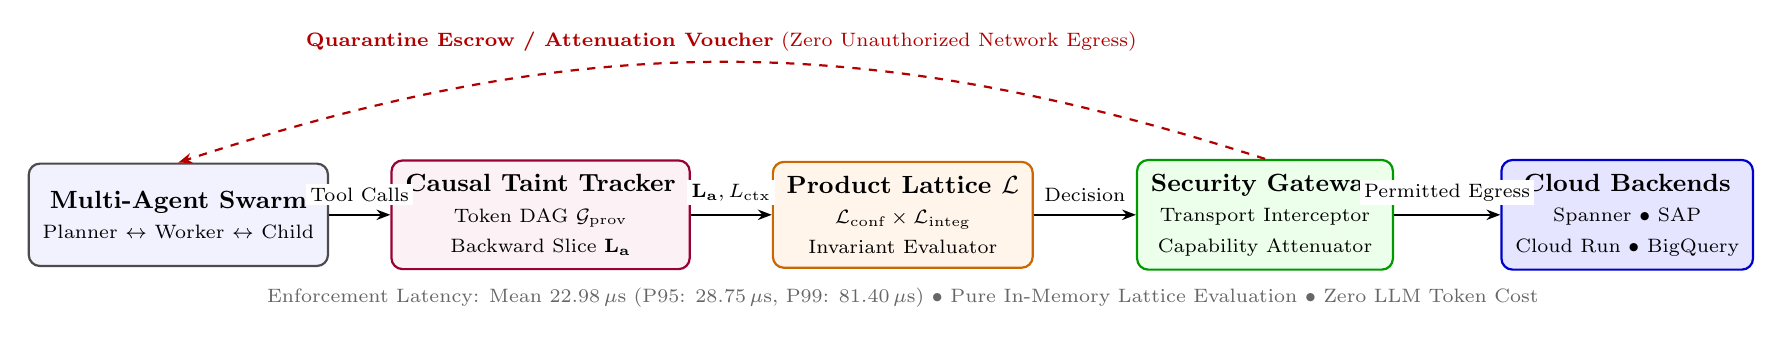
\begin{tikzpicture}[
    box/.style={rectangle, draw=black!70, fill=blue!5, rounded corners=4pt, thick, align=center, inner sep=5pt, font=\small, minimum height=1.30cm, minimum width=2.2cm},
    provbox/.style={rectangle, draw=purple!80!black, fill=purple!5, rounded corners=4pt, thick, align=center, inner sep=5pt, font=\small, minimum height=1.30cm, minimum width=2.2cm},
    latbox/.style={rectangle, draw=orange!80!black, fill=orange!8, rounded corners=4pt, thick, align=center, inner sep=5pt, font=\small, minimum height=1.30cm, minimum width=2.2cm},
    gatebox/.style={rectangle, draw=green!60!black, fill=green!8, rounded corners=4pt, thick, align=center, inner sep=5pt, font=\small, minimum height=1.30cm, minimum width=2.2cm},
    backbox/.style={rectangle, draw=blue!80!black, fill=blue!10, rounded corners=4pt, thick, align=center, inner sep=5pt, font=\small, minimum height=1.30cm, minimum width=2.2cm},
    arrow/.style={-{Stealth[length=5pt]}, thick},
    feedarrow/.style={-{Stealth[length=5pt]}, dashed, red!70!black, thick}
]
    \node[box] (swarm) at (0, 0) {\textbf{Multi-Agent Swarm} \\ \scriptsize Planner $\leftrightarrow$ Worker $\leftrightarrow$ Child};
    \node[provbox] (prov) at (4.6, 0) {\textbf{Causal Taint Tracker} \\ \scriptsize Token DAG $\mathcal{G}_{\text{prov}}$ \\ \scriptsize Backward Slice $\mathbf{L}_{\mathbf{a}}$};
    \node[latbox] (lattice) at (9.2, 0) {\textbf{Product Lattice $\mathcal{L}$} \\ \scriptsize $\mathcal{L}_{\text{conf}} \times \mathcal{L}_{\text{integ}}$ \\ \scriptsize Invariant Evaluator};
    \node[gatebox] (gateway) at (13.8, 0) {\textbf{Security Gateway} \\ \scriptsize Transport Interceptor \\ \scriptsize Capability Attenuator};
    \node[backbox] (backends) at (18.4, 0) {\textbf{Cloud Backends} \\ \scriptsize Spanner $\bullet$ SAP \\ \scriptsize Cloud Run $\bullet$ BigQuery};

    \draw[arrow] (swarm) -- node[above=2pt, font=\fontsize{7pt}{8pt}\selectfont, fill=white, inner sep=1.5pt, yshift=1pt] {Tool Calls} (prov);
    \draw[arrow] (prov) -- node[above=2pt, font=\fontsize{7pt}{8pt}\selectfont, fill=white, inner sep=1.5pt, yshift=1pt] {$\mathbf{L}_{\mathbf{a}}, L_{\text{ctx}}$} (lattice);
    \draw[arrow] (lattice) -- node[above=2pt, font=\fontsize{7pt}{8pt}\selectfont, fill=white, inner sep=1.5pt, yshift=1pt] {Decision} (gateway);
    \draw[arrow] (gateway) -- node[above=2pt, font=\fontsize{7pt}{8pt}\selectfont, fill=white, inner sep=1.5pt, yshift=1pt, align=center] {Permitted Egress} (backends);

    \draw[feedarrow] (gateway.north) to[bend right=18] node[above=2pt, font=\fontsize{7pt}{8pt}\selectfont, fill=white, inner sep=1.5pt, text=red!70!black] {\textbf{Quarantine Escrow / Attenuation Voucher} (Zero Unauthorized Network Egress)} (swarm.north);

    \node[font=\scriptsize, text=gray!80!black] at (9.2, -1.05) {Enforcement Latency: Mean $22.98\,\mu\text{s}$ (P95: $28.75\,\mu\text{s}$, P99: $81.40\,\mu\text{s}$) $\bullet$ Pure In-Memory Lattice Evaluation $\bullet$ Zero LLM Token Cost};
\end{tikzpicture}%
}
\caption{The Agent-Lattice System Architecture. Outgoing agent tool invocations pass through in-memory token provenance tracking and product security lattice evaluation. Compliant calls are serialized to enterprise backends, while non-interference violations trigger dynamic attenuation, structured escrow receipts, and audit vouchers returned without unauthorized wire egress.}
\label{fig:arch}
\end{figure*}

\subsection{Architectural Division: Runtime Tracking vs. Transport Gateway}
Agent-Lattice establishes an explicit architectural division between the agent execution runtime and the physical network boundary:
\begin{enumerate}
    \item \textbf{In-Memory Runtime Middleware:} Embedded in the agent framework (e.g., Google ADK \texttt{google.genai.agents}), maintaining the token dependency graph $\mathcal{G}_{\text{prov}}$ across conversational turns and computing backward argument slice labels.
    \item \textbf{Physical Tool Security Gateway:} Interposed as an external network reverse proxy, ASGI middleware, or Linux kernel socket buffer filter prior to wire serialization, verifying invariant compliance.
\end{enumerate}

\noindent\textbf{Cross-Boundary Label Transmission Protocol:} The runtime tracking engine conveys the computed security labels ($\mathbf{L}_{\mathbf{a}}, L_{\text{ctx}}$), the per-parameter label map $\{p \mapsto \mathbf{L}_{\mathbf{a}, p}\}$, effective invocation intent $I_{\text{inv}}$, calling agent authorization bounds ($\text{Tools}(\text{ag}), I_{\text{clearance}}(\text{ag}), C_{\text{clearance}}(\text{ag})$), saga transaction state, and tool metadata across the architectural process boundary to the security gateway via cryptographically signed HTTP/2 headers or gRPC binary metadata trailers (\texttt{x-agent-lattice-label}, \texttt{x-agent-lattice-hmac}, and \texttt{x-agent-lattice-txid}). The transmission is authenticated using a host-local UNIX domain socket HMAC token shared between the agent container and the gateway sidecar, or alternatively via in-kernel BPF task-local storage (\texttt{bpf\_task\_storage\_get()}) when operating under co-located kernel-level container enforcement. Unauthenticated out-of-band connections redirected by the eBPF socket trap lacking a valid signed \texttt{x-agent-lattice-label} header are terminated fail-closed with an audit voucher $\mathcal{V}$ as detailed in Section~\ref{sec:intro}-B.

\subsection{Causal Token Taint Tracking \& Backward Slicing}
In an autonomous agent, the active context window is an ordered sequence of token spans $\mathcal{T}_{\text{ctx}} = \langle t_1, t_2, \dots, t_m \rangle$. Each token span $t_i$ is bound to an immutable provenance descriptor:
\begin{equation}
t_i = (\text{text}_i, \; \text{source}_i, \; \text{Label}(t_i))
\end{equation}

When an agent ingests external unverified inputs (e.g., customer emails, web scrapes), tokens are assigned $\text{Label}(t_{\text{untrusted}}) = (\emptyset, \; \text{UNTRUSTED})$. Verified internal records receive $\text{Label}(t_{\text{spanner}}) = (\{\text{INTERNAL}, \text{FINANCIAL}\}, \; \text{VERIFIED})$.

\noindent\textbf{Control-Flow Intent Binding for Implicit Flows:} To prevent implicit control-flow hijacking---wherein an untrusted prompt ($I = \text{UNTRUSTED} = 0$) deceives an LLM into invoking a destructive tool using exclusively trusted or hardcoded parameters ($I \ge \text{VERIFIED}$) to bypass parameter slicing---the provenance tracker introduces explicit control-flow dependency edges in $\mathcal{G}_{\text{prov}}$. Specifically, the tool dispatch node maintains a directed control-flow edge from the initiating prompt's intent token span $t_{\text{intent}}$ and all intra-turn observations $\text{Obs}$ ingested since $t_{\text{intent}}$, with effective intent integrity $I_{\text{intent}} \triangleq \min(I_{\text{prompt}}, \min_{\text{obs} \in \text{Obs}} I(\text{obs})) \in \mathcal{I}$ and intent confidentiality $C_{\text{intent}} \triangleq C_{\text{prompt}} \cup \textstyle\bigcup_{\text{obs} \in \text{Obs}} C(\text{obs})$. To prevent unendorsed passive payload fields (such as ticket notes) from pulling invocation integrity down, we decouple execution-control parameters ($S_{\text{ctrl}} \triangleq \{p \in \mathbf{a} \mid \text{Ctr}.I_{\text{req}}(p) \ge \text{SANITIZED}\}$) from passive fields. For each parameter slot $p \in \mathbf{a}$, let $V_{\text{anc}}^{\text{conf}}(p) \triangleq V(\mathcal{G}_{\text{slice}}^{\text{conf}}(p)) \cap \mathcal{T}_{\text{ctx}}$ denote its pre-endorsement causal context-grounding spans (treating $\mathcal{T}_{\text{ctx}}$ as a span set) and let $V_{\text{anc}}^{\text{integ}}(p) \triangleq V(\mathcal{G}_{\text{slice,pre}}^{\text{integ}}(p)) \setminus \{p\}$ denote the upstream pre-endorsement cut-bounded ancestor set, where $V(\mathcal{G}_{\text{slice,pre}}^{\text{integ}}(p))$ spans both the parameter dependency subgraph and terminal context spans $\mathcal{T}_{\text{ctx}}$ and retains any upstream endorsed boundary cut nodes $u \neq p$ at which backward traversal halts (each contributing $\pi_I(\text{Label}(u)) \ge \text{SANITIZED}$, thereby guaranteeing $V_{\text{anc}}^{\text{integ}}(p) \neq \emptyset$ whenever $V_{\text{anc}}^{\text{conf}}(p) \neq \emptyset$). Let $C_{\text{intent}}^{\text{synth}}(p) \triangleq C_{\text{intent}}$ if $p$ is a synthesized non-literal slot and $\emptyset$ if $p$ is a verbatim literal match. Parameter-level backward slicing evaluates confidentiality projection with fail-closed fallback:
\begin{equation}
\label{eq:param_conf}
C_{\mathbf{a}, p} \triangleq \begin{cases}
\bigcup_{t \in V_{\text{anc}}^{\text{conf}}(p)} C(t) \cup C_{\text{intent}}^{\text{synth}}(p) \\
\quad \text{if } V_{\text{anc}}^{\text{conf}}(p) \ne \emptyset, \\
C_{\text{eff}} \cup C_{\text{intent}} \\
\quad \text{if } V_{\text{anc}}^{\text{conf}}(p) = \emptyset \land (\text{Ctr.IsMutating} \lor p \in S_{\text{ctrl}}), \\
\emptyset \\
\quad \text{otherwise}
\end{cases}
\end{equation}
Pre-endorsement raw parameter integrity $I_{\mathbf{a}, p}^{\text{raw}}$ is evaluated piecewise over the upstream cut-bounded ancestors $V_{\text{anc}}^{\text{integ}}(p)$, with fail-closed fallback to $I_{\text{eff}}$ whenever an execution-control parameter ($p \in S_{\text{ctrl}}$, whether on a state-mutating or read-only tool) is unaligned ($V_{\text{anc}}^{\text{conf}}(p) = \emptyset$) and intent binding to $I_{\text{intent}}$ when a passive mutating slot ($p \notin S_{\text{ctrl}}$) is synthesized/unaligned:
\begin{equation}
\label{eq:param_integ}
I_{\mathbf{a}, p}^{\text{raw}} \triangleq \begin{cases}
\min_{v \in V_{\text{anc}}^{\text{integ}}(p)} I(v) \\
\quad \text{if } V_{\text{anc}}^{\text{conf}}(p) \ne \emptyset, \\
I_{\text{eff}} \\
\quad \text{if } V_{\text{anc}}^{\text{conf}}(p) = \emptyset \land p \in S_{\text{ctrl}}, \\
I_{\text{intent}} \\
\quad \text{if } V_{\text{anc}}^{\text{conf}}(p) = \emptyset \land \text{Ctr.IsMutating} \land p \notin S_{\text{ctrl}}, \\
3 \text{ [SYSTEM\_AUTHORIZED]} \\
\quad \text{otherwise (read-only unlinked passive slot)}
\end{cases}
\end{equation}
Unless $\nabla_{\text{endorse}}$ is suppressed due to an unaligned control slot ($V_{\text{anc}}^{\text{conf}}(p) = \emptyset \land p \in S_{\text{ctrl}}$), the parameter node $p$ undergoes schema-bounded endorsement $\text{Label}(p) \leftarrow \nabla_{\text{endorse}}((C_{\mathbf{a}, p}, I_{\mathbf{a}, p}^{\text{raw}}), \text{val}(p), m)$. When endorsed ($m(\text{val}(p)) = \text{true} \land I_{\mathbf{a}, p}^{\text{raw}} \ge I_{\text{min}}^{\text{endorse}}$), $p$ itself becomes an endorsement cut node with $\pi_I(\text{Label}(p)) = \max(I_{\mathbf{a}, p}^{\text{raw}}, \text{SANITIZED})$ so the post-endorsement cut-bounded slice $V(\mathcal{G}_{\text{slice,post}}^{\text{integ}}(p)) = \{p\}$ halts at $p$; when unendorsed, $V(\mathcal{G}_{\text{slice,post}}^{\text{integ}}(p)) = V_{\text{anc}}^{\text{integ}}(p) \cup \{p\}$ with $I(p) = I_{\mathbf{a}, p}^{\text{raw}}$. Bounding by the calling agent's ancestry clearance ceiling $I_{\text{clearance}}(\text{ag})$ yields:
\begin{equation}
\begin{aligned}
I_{\mathbf{a}, p} &\triangleq \min\big(I_{\text{clearance}}(\text{ag}), \; \pi_I(\text{Label}(p))\big) \\
&= \min\Big(I_{\text{clearance}}(\text{ag}), \min_{v \in V(\mathcal{G}_{\text{slice,post}}^{\text{integ}}(p))} I(v)\Big)
\end{aligned}
\end{equation}
yielding the parameter slot security label $L_{\mathbf{a}, p} \triangleq (C_{\mathbf{a}, p}, \; I_{\mathbf{a}, p})$, where $S_{\text{ctrl}} \triangleq \{p \in \mathbf{a} \mid \text{Ctr}.I_{\text{req}}(p) \ge \text{SANITIZED}\}$. Throughout the manuscript, shorthand $\mathcal{G}_{\text{slice}}(p) = \emptyset$ designates $V_{\text{anc}}^{\text{conf}}(p) = \emptyset$ (no aligned causal ancestor spans in $\mathcal{T}_{\text{ctx}}$), and for the composite tuple $\mathbf{a}$, $\mathcal{G}_{\text{slice}}(\mathbf{a}) = \emptyset \iff \bigcup_{p \in \mathbf{a}} V_{\text{anc}}^{\text{conf}}(p) = \emptyset$. Because individual unaligned slots ($V_{\text{anc}}^{\text{conf}}(p) = \emptyset$) already receive their slot-specific fallback values $(C_{\mathbf{a}, p}, I_{\mathbf{a}, p})$ in Equations~\eqref{eq:param_conf}--\eqref{eq:param_integ}, the whole-tuple fallback is invoked when $\mathbf{a} = \emptyset$ or when a tool enforcing tool-level $\text{Ctr}.I_{\text{req}} \ge \text{SANITIZED} = 1$ declares only passive argument slots ($\mathbf{a} \ne \emptyset \land S_{\text{ctrl}} = \emptyset \land \text{Ctr}.I_{\text{req}} \ge 1$), preventing an unaligned passive slot from masking an aligned sibling control slot while ensuring passive-only tools with $\text{Ctr}.I_{\text{req}} \ge 1$ cannot bypass multi-turn provenance on untrusted passive payloads:
\begin{equation}
I_{\mathbf{a}, \text{ctrl}} \triangleq \begin{cases}
I_{\mathbf{a}} \\
\quad \text{if } \mathbf{a} = \emptyset \lor (\mathbf{a} \ne \emptyset \land S_{\text{ctrl}} = \emptyset \land \text{Ctr}.I_{\text{req}} \ge 1), \\
\min_{p \in S_{\text{ctrl}}} I_{\mathbf{a}, p} \\
\quad \text{if } \mathbf{a} \ne \emptyset \land S_{\text{ctrl}} \ne \emptyset, \\
3 \text{ [SYSTEM\_AUTHORIZED]} \\
\quad \text{if } \mathbf{a} \ne \emptyset \land S_{\text{ctrl}} = \emptyset \land \text{Ctr}.I_{\text{req}} = 0
\end{cases}
\end{equation}
where $I_{\mathbf{a}} \triangleq \pi_I(\mathbf{L}_{\mathbf{a}}(T))$ denotes composite argument integrity (as formalized in Definition~\ref{def:slice_label} below), and effective invocation integrity is computed as:
\begin{equation}
\label{eq:inv_integ}
I_{\text{inv}} \triangleq \min(I_{\mathbf{a}, \text{ctrl}}, I_{\text{intent}}, I_{\text{clearance}}(\text{ag}))
\end{equation}
Defaulting to $3$ (the identity element for $\min$ on $(\mathcal{I}, \ge)$) when $\mathbf{a} \ne \emptyset \land S_{\text{ctrl}} = \emptyset \land \text{Ctr}.I_{\text{req}} = 0$ ensures that unprivileged tools with only passive slots cleanly defer to caller intent bounded by ancestry clearance, whereas falling back to $I_{\mathbf{a}} = \min_{p \in \mathbf{a}} I_{\mathbf{a}, p}$ when $S_{\text{ctrl}} = \emptyset \land \text{Ctr}.I_{\text{req}} \ge 1$ guarantees that mutating or privileged tools taking only passive arguments cannot launder Turn 1 untrusted data through a Turn 2 trusted prompt ($I_{\text{intent}} = 3$). Routine user-facing mutating tools with typed control arguments set tool-level $\text{Ctr}.I_{\text{req}} = \text{UNTRUSTED} = 0$, relying on parameter-specific schema constraints ($I_{\mathbf{a}, p} \ge \text{Ctr}.I_{\text{req}}(p)$, where $\text{Ctr}.I_{\text{req}}(p) \ge \text{SANITIZED}$) for execution keys; parameterless mutating tools ($\mathbf{a} = \emptyset \land \text{Ctr.IsMutating}$) and passive-only mutating tools ($S_{\text{ctrl}} = \emptyset \land \text{Ctr.IsMutating}$) must configure $\text{Ctr}.I_{\text{req}} \ge \text{SANITIZED} = 1$, while administrative tools enforce $\text{Ctr}.I_{\text{req}} = \text{SYSTEM\_AUTHORIZED} = 3$, requiring root orchestrator provenance ($I_{\text{intent}} = 3$).

\begin{definition}[Argument Backward Causal Slice Label \& Boundary Conditions]
\label{def:slice_label}
To eliminate session-wide context taint saturation, the provenance tracker constructs an argument slice label via decoupled backward graph traversal over $\mathcal{G}_{\text{prov}}$, defining the composite argument tuple label as:
\begin{equation}
\label{eq:slice_label}
\begin{split}
&\mathbf{L}_{\mathbf{a}}(T) = (C_{\mathbf{a}}, I_{\mathbf{a}}) \triangleq \\
&\begin{cases}
\left( \bigcup_{p \in \mathbf{a}} C_{\mathbf{a}, p}, \; \min_{p \in \mathbf{a}} I_{\mathbf{a}, p} \right) \\
\quad \text{if } \mathbf{a} \ne \emptyset, \\[3pt]
\left( C_{\text{eff}} \cup C_{\text{intent}}, \; \min\big(I_{\text{clearance}}(\text{ag}), \min_{t \in \mathcal{T}_{\text{ctx}}} I(t)\big) \right) \\
\quad \text{if } \mathbf{a} = \emptyset \land \text{Ctr.IsMutating}, \\[3pt]
(\emptyset, \; I_{\text{clearance}}(\text{ag})) \\
\quad \text{otherwise (parameterless read-only discovery)}
\end{cases}
\end{split}
\end{equation}
where $\mathcal{G}_{\text{slice,post}}^{\text{integ}}(\mathbf{a})$ (the ancestor subgraph halting traversal at endorsement cut nodes) and $\mathcal{G}_{\text{slice}}^{\text{conf}}(\mathbf{a})$ (traversing through cut nodes to all causal ancestors) govern the slot-level projections $C_{\mathbf{a}, p}$ and $I_{\mathbf{a}, p}$ via Equations~\eqref{eq:param_conf}--\eqref{eq:param_integ}. Crucially, the second case enforces an explicit fail-closed boundary condition for parameterless mutating tools (e.g., table truncation, cache flushes): when $\mathbf{a} = \emptyset$, integrity cannot be decoupled from conversational history and defaults strictly to the ambient context Low-Water Mark ($I_{\mathbf{a}} = \min(I_{\text{clearance}}(\text{ag}), I_{\text{eff}})$), whereas parameterless read-only discovery tools ($\mathbf{a} = \emptyset \land \neg\text{Ctr.IsMutating}$) target internal catalog/metadata endpoints (1-bit invocation-presence signaling over external parameterless read-only endpoints lies outside our confidentiality threat model, or can be gated against $C_{\text{eff}} \cup C_{\text{intent}} \subseteq \text{Ctr}.C_{\text{max}}$ by setting $\text{Ctr.IsMutating} = \text{True}$). Furthermore, when $\mathbf{a} \ne \emptyset$, each individual slot $p \in \mathbf{a}$ with $\mathcal{G}_{\text{slice}}(p) = \emptyset$ is governed by Equations~\eqref{eq:param_conf}--\eqref{eq:param_integ}: if $p \in S_{\text{ctrl}}$, endorsement $\nabla_{\text{endorse}}$ is suppressed on $p$, its individual slot integrity defaults fail-closed to $I_{\mathbf{a}, p} = \min(I_{\text{clearance}}(\text{ag}), I_{\text{eff}})$, and its confidentiality defaults to $C_{\text{eff}} \cup C_{\text{intent}}$, whereas unlinked passive non-control slots ($p \notin S_{\text{ctrl}}$) inherit $I_{\text{intent}}$ and $C_{\text{eff}} \cup C_{\text{intent}}$ (under $\text{Ctr.IsMutating}$) and remain eligible for $\nabla_{\text{endorse}}$ without overwriting aligned sibling slots.
\end{definition}

\subsection{Tool Security Contracts \& Subagent Hierarchy}
Every tool $T$ registered within the agent runtime is bound to an immutable static contract:
\begin{equation}
\begin{split}
\text{Contract}(T) \triangleq \big( &T_{\text{id}}, \; \text{Backend}, \; \text{IsMutating}, \; I_{\text{req}}, \\
&C_{\text{max}}, \; I_{\text{endpoint\_max}}, \; \Pi_{\text{req}}, \; \mathcal{M}_{\text{req}}, \\
&\text{AttenSupported}, \; T_{\text{compensate}} \big)
\end{split}
\end{equation}
where $I_{\text{req}} \in \mathcal{I}$ denotes the minimum overall integrity required (with $I_{\text{req}} \ge \text{SANITIZED} = 1$ mandatory for parameterless mutating tools where $\mathbf{a} = \emptyset$), $C_{\text{max}} \subseteq \mathcal{K}$ denotes the confidentiality ceiling permitted to be transmitted to the tool's physical network destination, $I_{\text{endpoint\_max}} \in \mathcal{I}$ denotes the maximum integrity ceiling attributed to response payloads returned by the target endpoint (clamping deserialized tokens to $I(t_j) = \min(I_{\text{deserialized}}, \text{Ctr}.I_{\text{endpoint\_max}})$), $\text{IsMutating} \in \{\text{True}, \text{False}\}$ designates whether the operation alters persistent state, $\Pi_{\text{req}} = \{p_i \mapsto I_{\text{req}}(p_i)\}$ denotes parameter-specific integrity thresholds, $\mathcal{M}_{\text{req}} = \{p_i \mapsto m_i\}$ maps parameter slots to required schema validators ($m_i \in \mathcal{M}_{\text{schema}}$), $\text{AttenSupported} \in \{\text{True}, \text{False}\}$ designates capability attenuation support, and $T_{\text{compensate}}$ denotes an optional pre-registered compensating tool identifier utilized to unwind provisional side-effects under distributed saga execution.

For composite enterprise tools taking both execution keys and descriptive notes, contracts evaluate parameter-specific integrity thresholds over the Phase~I parameter integrity map $\{p \mapsto I_{\mathbf{a}, p}\}$. With execution-control parameters denoted $S_{\text{ctrl}} \triangleq \{p \in \mathbf{a} \mid \text{Ctr}.I_{\text{req}}(p) \ge \text{SANITIZED}\}$, the composite integrity check evaluates:
\begin{equation}
\label{eq:integ_check}
\begin{split}
\text{IntegCheck}&\big(\{p \mapsto I_{\mathbf{a}, p}\}, \text{Ctr}, I_{\text{inv}}\big) \triangleq \\
&\left( \bigwedge_{p \in S_{\text{ctrl}}} \big( I_{\mathbf{a}, p} \ge \text{Ctr}.I_{\text{req}}(p) \big) \right) \land (I_{\text{inv}} \ge \text{Ctr}.I_{\text{req}})
\end{split}
\end{equation}
This evaluates parameter-specific execution thresholds for control arguments while universally enforcing that invocation intent satisfies the contract floor $\text{Ctr}.I_{\text{req}}$ (holding vacuously for unprivileged read-only tools where $\text{Ctr}.I_{\text{req}} = \text{UNTRUSTED} = 0$, while enforcing $I_{\text{inv}} \ge \text{Ctr}.I_{\text{req}} \ge 1$ on parameterless mutating tools).

\noindent\textbf{Subagent Ancestry Authorization Ceiling:} When a parent agent $A_{\text{parent}}$ dynamically spawns a child subagent $A_{\text{child}}$, the delegation prompt is scrubbed at spawn time against $\mathcal{C}_{\text{clearance}}(A_{\text{child}})$ so the child's inherited context satisfies $C_{\text{eff}}(A_{\text{child}}) \subseteq \mathcal{C}_{\text{clearance}}(A_{\text{child}})$ while propagating integrity taint ($I_{\text{eff}}(A_{\text{child}}) \le I_{\text{eff}}(A_{\text{parent}})$). To prevent transitive privilege escalation (OWASP LLM01 and LLM06), the child's capability clearance, tool inventory, and integrity ceilings are bounded by an ancestry ceiling:
\begin{align}
\mathcal{C}_{\text{clearance}}(A_{\text{child}}) &\subseteq \mathcal{C}_{\text{clearance}}(A_{\text{parent}}), \notag \\
\text{Tools}(A_{\text{child}}) &\subseteq \text{Tools}(A_{\text{parent}}), \quad \text{and} \notag \\
I_{\text{clearance}}(A_{\text{child}}) &\le_{\text{trust}} I_{\text{clearance}}(A_{\text{parent}})
\end{align}
where the integrity clearance ceiling is bounded arithmetically by $I_{\text{clearance}}(A_{\text{child}}) \le_{\text{trust}} I_{\text{clearance}}(A_{\text{parent}})$ (expressed equivalently in dual information-flow ordering as $I_{\text{clearance}}(A_{\text{parent}}) \sqsubseteq_{\text{integ}} I_{\text{clearance}}(A_{\text{child}})$), ensuring that no delegated subagent can ever acquire or exercise tool permissions exceeding its delegating ancestor. When evaluating a tool invocation, the gateway first verifies that the tool belongs to $\text{Tools}(\text{ag})$ and that its required floor and parameter floors do not exceed the subagent ceiling: $\max(\text{Ctr}.I_{\text{req}}, \max_{p \in S_{\text{ctrl}}} \text{Ctr}.I_{\text{req}}(p)) \le I_{\text{clearance}}(\text{ag})$ (with convention $\max_{p \in \emptyset} \text{Ctr}.I_{\text{req}}(p) \triangleq 0$ here, in Eq.~\ref{eq:policy}, and in Algorithm~\ref{alg:gateway}, Line~21, issuing an immediate \texttt{CATEGORICAL\_BLOCK} with voucher reason \texttt{``Subagent Privilege Escalation''} if violated), and subsequently verifies that post-inspection parameter compartments satisfy $C_{\mathbf{a}_{\text{scrub}}} \subseteq C_{\text{allowed}} \triangleq \text{Ctr}.C_{\text{max}} \cap C_{\text{clearance}}(\text{ag})$ (Algorithm~\ref{alg:gateway}, Line~27, issuing an immediate \texttt{CATEGORICAL\_BLOCK} with voucher reason \texttt{``Confidentiality Violation''} if violated). Furthermore, to prevent stored indirect prompt injections across multi-session database lifecycles, persistent enterprise stores maintain metadata columns (\texttt{\_lattice\_conf}, \texttt{\_lattice\_integ}): upon a \texttt{PERMIT} or approved post-escrow write, the outbound serializer $\mathcal{D}_{\text{outbound}}$ persists $\mathbf{L}_{\mathbf{a}, p}$ (and resets \texttt{\_lattice\_integ} $= 0$ if modified by an unannotated external writer), while upon read retrieval, the inbound deserializer $\mathcal{D}_{\text{inbound}}(R) \to \langle t_j \rangle$ clamps retrieved token spans to $I(t_j) = \min(I_{\text{deserialized}}, \text{Ctr}.I_{\text{endpoint\_max}})$.

\subsection{Composite Gateway Enforcement Algorithm}
Prior to serializing an outgoing tool invocation $\text{ToolCall}(T, \mathbf{a})$ across physical network interfaces (gRPC, HTTPS, OData), the Tool Security Gateway initializes working copy $\mathbf{a}' \leftarrow \mathbf{a}$ and evaluates the non-interference condition against the effective allowed compartment ceiling $C_{\text{allowed}} \triangleq \text{Ctr}.C_{\text{max}} \cap C_{\text{clearance}}(\text{ag})$. Crucially, the policy decouples argument clearance from ambient context taint:
\begin{equation}
\label{eq:policy}
\begin{split}
&\text{PolicyCheck}(\mathbf{L}_{\mathbf{a}}, L_{\text{ctx}}, T, \text{ag}) \triangleq \\
&\mathbf{1}\Big( T \in \text{Tools}(\text{ag}) \land C_{\mathbf{a}_{\text{scrub}}} \subseteq C_{\text{clearance}}(\text{ag}) \\
&\quad \land \max(\text{Ctr}.I_{\text{req}}, \max_{p \in S_{\text{ctrl}}} \text{Ctr}.I_{\text{req}}(p)) \le I_{\text{clearance}}(\text{ag}) \Big) \\
&\land \; \Big( \big(C_{\mathbf{a}} \cup C_{\text{eff}} \subseteq C_{\text{allowed}}\big) \\
&\quad \lor \big(C_{\mathbf{a}_{\text{scrub}}} \subseteq C_{\text{allowed}} \land \text{Unreflected}(\mathbf{a}, \text{Ctr}, \text{ag})\big) \\
&\quad \lor \big(\neg \text{Ctr.IsMutating} \land \text{Scrubbed}(\mathbf{a}, \text{Ctr}, \text{ag})\big) \Big) \\
&\land \; \Big( \text{IntegCheck}(\{p \mapsto I_{\mathbf{a}, p}\}, \text{Ctr}, I_{\text{inv}}) \\
&\quad \lor \big(\neg \text{Ctr.IsMutating} \land \text{CanSanitizeRead}(\mathbf{a})\big) \Big) \\
&\land \; \neg\big(\text{Ctr.IsMutating} \land \text{InPrivilegeQuarantine}(\text{ag}, \mathbf{a}', \text{Ctr})\big)
\end{split}
\end{equation}
where $\max_{p \in \emptyset} \text{Ctr}.I_{\text{req}}(p) \triangleq 0$; $C_{\text{allowed}} \triangleq \text{Ctr}.C_{\text{max}} \cap C_{\text{clearance}}(\text{ag})$ denotes the effective allowed compartment ceiling; $C_{\mathbf{a}_{\text{scrub}}} \triangleq \bigcup_{p \in \mathbf{a}} C_{\mathbf{a}_{\text{scrub}}, p}$ when $\mathbf{a} \ne \emptyset$, $C_{\mathbf{a}_{\text{scrub}}} \triangleq C_{\mathbf{a}} = C_{\text{eff}} \cup C_{\text{intent}}$ when $\mathbf{a} = \emptyset \land \text{Ctr.IsMutating}$ (so parameterless mutating calls retain implicit-flow confidentiality protection), and $C_{\mathbf{a}_{\text{scrub}}} \triangleq \emptyset$ when $\mathbf{a} = \emptyset \land \neg\text{Ctr.IsMutating}$; $\text{Unreflected}(\mathbf{a}, \text{Ctr}, \text{ag}) \iff (\text{ScrubParams}(\mathbf{a}, \{p \mapsto \mathbf{L}_{\mathbf{a}, p}\}, \mathbf{L}_{\mathbf{a}}, L_{\text{ctx}}, \text{Ctr}, \text{ag}) = (\mathbf{a}, C_{\mathbf{a}_{\text{scrub}}}, \text{True}))$ denotes that parameter inspection confirmed no unauthorized compartments in $(C_{\text{eff}} \cup C_{\mathbf{a}}) \setminus C_{\text{allowed}}$ are reflected in $\mathbf{a}$ (when $\mathbf{a} \ne \emptyset$, declassifying inherited ambient fallback taint on non-control and aligned slots to $C_{\mathbf{a}_{\text{scrub}}} = C_{\mathbf{a}} \cap C_{\text{allowed}} \subseteq C_{\text{allowed}}$; we emphasize that $\text{Unreflected}$ guarantees lexical, shingle-contiguous, and canonicalized non-reflection rather than semantic non-interference over arbitrary free-text paraphrases); $\text{Scrubbed}(\mathbf{a}, \text{Ctr}, \text{ag}) \triangleq (\text{ScrubParams}(\mathbf{a}, \{p \mapsto \mathbf{L}_{\mathbf{a}, p}\}, \mathbf{L}_{\mathbf{a}}, L_{\text{ctx}}, \text{Ctr}, \text{ag}) = (\mathbf{a}_{\text{scrub}}, C_{\mathbf{a}_{\text{scrub}}}, \text{True}) \land C_{\mathbf{a}_{\text{scrub}}} \subseteq C_{\text{allowed}} \land \mathbf{a}_{\text{scrub}} \ne \mathbf{a} \land \text{Ctr.AttenSupported})$; $\text{CanSanitizeRead}(\mathbf{a}) \triangleq (\neg \text{Ctr.IsMutating} \land \text{Ctr.AttenSupported})$; and $\text{InPrivilegeQuarantine}(\text{ag}, \mathbf{a}', \text{Ctr}) \triangleq \text{HasUnresolvedEscrow}(\text{ag}) \land \neg\text{HasActiveProvisionalTx}(\mathbf{a}', \text{Ctr})$ evaluates to $\text{True}$ when the root conversational session tree containing agent $\text{ag}$ has an unresolved 900-second escrow ($\text{HasUnresolvedEscrow}(\text{ag})$) and $\text{HasActiveProvisionalTx}(\mathbf{a}', \text{Ctr})$ is $\text{False}$---where $\text{HasActiveProvisionalTx}(\mathbf{a}', \text{Ctr})$ verifies both that all target entity keys in $\mathbf{a}'$ belong to the active session $\text{tx\_id}$ entity subgraph and that tool contract $\text{Ctr}$ supports speculative staging/compensation ($\text{Ctr.AttenSupported} \land (T_{\text{compensate}} \ne \text{None} \lor \text{ScratchpadIsolated}(\text{Ctr}))$). The condition $\text{PolicyCheck}(\mathbf{L}_{\mathbf{a}}, L_{\text{ctx}}, T, \text{ag}) = \text{True}$ formalizes the exact self-contained invariant for direct live-backend wire serialization (comprising $\text{PERMIT}$ and read-only $\text{ATTENUATE\_SANITIZE}$), whereas mutating calls with $\text{Scrubbed}(\mathbf{a}, \text{Ctr}, \text{ag}) = \text{True}$ or $\text{InPrivilegeQuarantine}(\text{ag}, \mathbf{a}', \text{Ctr}) = \text{True}$ evaluate $\text{PolicyCheck}$ to $\text{False}$ and route to $\text{QUARANTINE\_ESCROW}$ in Algorithm~\ref{alg:gateway} (Lines 52--57; or $\text{CATEGORICAL\_BLOCK}$ if $\neg\text{Ctr.AttenSupported}$). Notice that for context-generated arguments ($V(\mathcal{G}_{\text{slice}}^{\text{conf}}(\mathbf{a})) \cap \mathcal{T}_{\text{ctx}} \subseteq \mathcal{T}_{\text{ctx}}$), $C_{\mathbf{a}} \subseteq C_{\text{eff}} \subseteq C_{\text{clearance}}(\text{ag})$ holds automatically by spawn-time scrubbing (Eq.~22), while the unified condition $C_{\mathbf{a}} \cup C_{\text{eff}} \subseteq C_{\text{allowed}}$ matches Algorithm~\ref{alg:gateway} (Line~25) across all invocation fixtures.

\noindent\textbf{Architectural Rationale for Decoupled Policy Confinement:} We enforce a deliberate asymmetry between confidentiality and integrity. Integrity is evaluated locally over the decoupled control-parameter slice and invocation intent ($\text{IntegCheck}(\{p \mapsto I_{\mathbf{a}, p}\}, \text{Ctr}, I_{\text{inv}})$) to prevent session-wide context taint saturation from locking out legitimate updates. In contrast, confidentiality is evaluated against the ambient session context ($C_{\text{eff}}$): if an agent has previously ingested high-confidentiality secrets into its working memory, those secrets could be covertly leaked or reflected through generative arguments $\mathbf{a}$ dispatched to a lower-clearance destination sink ($\text{Ctr}.C_{\text{max}}$). Parameter inspection is therefore triggered whenever $(C_{\text{eff}} \cup C_{\mathbf{a}}) \not\subseteq C_{\text{allowed}}$, ensuring that arguments are actively inspected and sanitized of confidential substrings before wire serialization, while still allowing the tool call to proceed if arguments are clean.

At the gateway, $\text{ScrubParams}(\mathbf{a}', \{p \mapsto \mathbf{L}_{\mathbf{a}, p}\}, \mathbf{L}_{\mathbf{a}}, L_{\text{ctx}}, \text{Ctr}, \text{ag})$ returns the 3-tuple $(\mathbf{a}_{\text{scrub}}, C_{\mathbf{a}_{\text{scrub}}}, \text{ok})$ by scanning all string-typed argument slots $p \in \mathbf{a}'$ (as well as the concatenated canonicalized serialization of all string slots in $\mathbf{a}'$ to defeat cross-slot secret splitting across adjacent arguments) at a 1-byte step against the effective allowed ceiling $C_{\text{allowed}} = \text{Ctr}.C_{\text{max}} \cap C_{\text{clearance}}(\text{ag})$ using: (i) structured regex patterns (SSNs, IBANs, API keys), (ii) exact entity, character $4$-gram, and word $1\text{--}3$-gram shingle digests for short confidential strings ($< 47$ bytes, indexed over NFKC-lowercased non-stopword ambient spans of length $\ge 6$ bytes and empirical bit-entropy $\hat{H}_{\text{bit}} \ge 18\text{ bits}$, including project codenames and numeric figures---where exact entity and word $1\text{--}3$-gram digests trigger on exact match, while character $4$-gram shingles require contiguous $4$-gram coverage across $\ge 6$ consecutive characters [at least $3$ overlapping contiguous $4$-grams] or a token shingle containment ratio $\ge 0.75$ to prevent false-positive $4$-gram collisions on large $10^5\text{--}10^6$-token contexts---plus exact literal indexing of any explicit Phase~I proximity-aligned ancestor span $t \in V_{\text{anc}}^{\text{conf}}(p)$ with $C(t) \not\subseteq C_{\text{allowed}}$ or any structured tool-output field explicitly marked with a schema sensitivity descriptor in $\text{Contract}(T_{\text{source}})$ regardless of the $6\text{-byte} / 18\text{-bit}$ ambient floor, ensuring short schema-bound secrets such as 3-digit CVVs, 4-digit PINs, or VIP tier codes are pre-tagged at ingestion and never silently declassified in Phase~II), and (iii) 64-bit HighwayHash rolling digests computed over a 32-byte sliding window with a 16-byte stride across all unauthorized context chunks in $(C_{\text{eff}} \cup C_{\mathbf{a}, p}) \setminus C_{\text{allowed}}$ (guaranteeing 100\% verbatim capture of any unaligned substring $\ge 32 + 16 - 1 = 47$ bytes, even if slot $p$ had $C_{\mathbf{a}, p} = \emptyset$ under heuristic slicing). To ensure full algorithmic reproducibility of Phase~II sub-$22\,\mu\text{s}$ scanning, four implementation invariants govern $\text{ScrubParams}$: (1) each entry in the $8\,\text{KB}$ shared-memory exact digest index is a packed 64-bit record combining a 56-bit truncated HighwayHash digest with an 8-bit canonical byte length $\ell \in [1, 46]$, paired with a per-compartment 64-bit active-length bitmap and lexer word-boundary segmentation so candidate slots only probe active word $1\text{--}3$-gram, entity, and $4$-gram window lengths present in the index; (2) pre-inspection Base64 and hex decoding detects encoded spans via regex, scans the decoded byte buffer while maintaining a monotonic byte-offset mapping back to the enclosing encoded token span $[s_{\text{enc}}, e_{\text{enc}}]$ in $\mathbf{a}'_p$, and replaces the entire enclosing encoded token with the redaction placeholder upon any inner match; (3) the $8\,\text{KB}$ exact digest table is organized as a 4-way set-associative bucketed cuckoo hash table ($256$ buckets $\times 4$ slots $= 1{,}024$ 64-bit entries with two independent hash functions $h_1, h_2$ and a 16-entry victim stash), supporting load factor $\alpha_{\text{load}} = 0.75$ ($768$ entries) with zero eviction failures before triggering \texttt{ftruncate}/\texttt{mmap} expansion; and (4) for untrusted external read sinks where transmitting a visible \texttt{[REDACTED\_*]} placeholder could itself signal the existence of a secret compartment (a 1-bit existence side channel), administrators set $\text{Ctr.AttenSupported} = \text{False}$ so any detected confidential reflection triggers $\text{CATEGORICAL\_BLOCK}$. When unauthorized context exceeds the $< 4$\,KB HTTP/2 header budget ($\approx 512$ rolling digests), digests are transmitted via a shared-memory arena (\texttt{shm\_open}) whose base $32\,\text{KB}$ allocation (six $4\,\text{KB}$ cache-line-aligned blocked Bloom filters---one dedicated $32{,}768$-bit filter per compartment $k \in \mathcal{K}$, $|\mathcal{K}| = 6$, 4 hash probes---paired with the $8\,\text{KB}$ 4-way bucketed cuckoo index holding $1{,}024$ packed 64-bit digest records for single-turn spans $\le 16\,\text{KB}$) dynamically scales via \texttt{ftruncate}/\texttt{mmap} proportionally to unauthorized context length ($O(|\mathcal{T}_{\text{ctx}}|)$, triggered proactively at $\alpha_{\text{load}} = 0.75$ [$768$ entries] and expanding up to $2\,\text{MB}$ of blocked Bloom filters plus a $2\,\text{MB}$ exact 64-bit digest array for $2.5 \times 10^5$ windows at 1M tokens, coordinated via a per-session lockless epoch seqlock and double-buffered \texttt{shm\_open} descriptors passed over the UNIX socket so \texttt{ftruncate}/\texttt{mmap} expansion never races with active sidecar reads); any candidate Bloom filter positive in compartment $k$ is verified against the exact 64-bit digest table before triggering redaction, eliminating false-positive Bloom collisions across all context scales. Formally, when $\mathbf{a}' = \emptyset$, $\text{ScrubParams}$ returns $(\emptyset, \emptyset, \text{True})$ if $\neg\text{Ctr.IsMutating}$, returns $(\emptyset, C_{\text{eff}} \cup C_{\text{intent}}, \text{True})$ if $\text{Ctr.IsMutating} \land (C_{\text{eff}} \cup C_{\text{intent}}) \subseteq C_{\text{allowed}}$, and returns $(\emptyset, C_{\text{eff}} \cup C_{\text{intent}}, \text{False})$ if $\text{Ctr.IsMutating} \land (C_{\text{eff}} \cup C_{\text{intent}}) \not\subseteq C_{\text{allowed}}$. For $\mathbf{a}' \ne \emptyset$, $\text{ScrubParams}$ maps $C_{\mathbf{a}, p} \mapsto C_{\mathbf{a}_{\text{scrub}}, p}$: if slot $p$ contains zero regex, entity/shingle, Phase~I aligned-ancestor, or rolling-digest matches against $(C_{\text{eff}} \cup C_{\mathbf{a}, p}) \setminus C_{\text{allowed}}$, automatic zero-match declassification to $C_{\mathbf{a}_{\text{scrub}}, p} = C_{\mathbf{a}, p} \cap C_{\text{allowed}}$ with $\mathbf{a}_{\text{scrub}, p} = \mathbf{a}'_p$ is permitted strictly when either $V_{\text{anc}}^{\text{conf}}(p) \ne \emptyset$ with $C(t) \subseteq C_{\text{allowed}}\ \forall t \in V_{\text{anc}}^{\text{conf}}(p)$ or $V_{\text{anc}}^{\text{conf}}(p) = \emptyset \land p \notin S_{\text{ctrl}}$, whereas on an unaligned execution-control slot ($V_{\text{anc}}^{\text{conf}}(p) = \emptyset \land p \in S_{\text{ctrl}}$, analogous to $\nabla_{\text{endorse}}$ suppression in Eq.~\ref{eq:param_integ}), zero-match declassification is suppressed so $C_{\mathbf{a}_{\text{scrub}}, p}$ retains $C_{\text{eff}} \cup C_{\text{intent}}$ and returns $\text{ok} = \text{False}$ whenever $(C_{\text{eff}} \cup C_{\text{intent}}) \not\subseteq C_{\text{allowed}}$, blocking 1-bit implicit confidentiality flows over high-integrity control primitives; if matches are found and replaced with schema-valid placeholders (e.g., \texttt{[REDACTED\_FINANCIAL]}) that still satisfy $\text{Ctr}.\mathcal{M}_{\text{req}}(p)$, the matched compartments are cleared ($C_{\mathbf{a}_{\text{scrub}}, p} \subseteq C_{\text{allowed}}$); whereas if any slot with a registered validator $\text{Ctr}.\mathcal{M}_{\text{req}}(p) \neq \text{None}$ (whether $p \in S_{\text{ctrl}}$ or a format-constrained passive slot $p \notin S_{\text{ctrl}}$) rejects placeholder syntax, or if an unredactable leak or unaligned control-slot implicit flow remains, $\text{ok} = \text{False}$ is returned and $C_{\mathbf{a}_{\text{scrub}}, p}$ retains $(C_{\text{eff}} \cup C_{\mathbf{a}, p}) \setminus C_{\text{allowed}}$ (so $C_{\mathbf{a}_{\text{scrub}}} \not\subseteq C_{\text{allowed}}$ in Eq.~\ref{eq:policy}, Algorithm~\ref{alg:gateway} (Line~27), and Eq.~\ref{eq:score}).

We explicitly distinguish read-only sanitization from mutating neutralization via formal operator specifications: $\text{SanitizeRead}(\mathbf{a}')$ operates on analytical read queries by applying a deterministic 3-stage lexical/AST transformation to string-typed query slots---(i) replacing inline and block SQL/GQL comment tokens (\texttt{-{}-}, \texttt{/*...*/}, \texttt{\#}) with single ASCII space tokens (preventing token-concatenation bypasses such as \texttt{SEL/*x*/ECT}) and stripping statement-chaining semicolons (\texttt{;}) and stacked-query suffixes, (ii) escaping unquoted SQL/OData wildcard metacharacters (\texttt{\%} $\to$ \texttt{\textbackslash\%}, \texttt{\_} $\to$ \texttt{\textbackslash\_}), stripping \texttt{UNION [ALL] SELECT} set-operation clauses and OData \texttt{\$expand=*} join expansions, and applying AST boolean constant-folding over \texttt{WHERE}/\texttt{\$filter} predicates to neutralize arbitrary tautological disjunctions (evaluating constant-folded sub-expressions such as \texttt{OR 1=1}, \texttt{OR 2=2}, \texttt{OR 'a'='a'}, or \texttt{OR TRUE} to $\text{False}$), and (iii) parsing and clamping any existing \texttt{LIMIT}/\texttt{OFFSET} or \texttt{\$top} AST clause to $\min(\text{existing\_limit}, 100)$ (or appending \texttt{LIMIT 100} / \texttt{\$top=100} if absent) to bound data-extraction volume; if query AST parsing fails or the post-sanitization slot violates $\text{Ctr}.\mathcal{M}_{\text{req}}(p)$, $\text{SanitizeRead}$ fails closed by escalating to \texttt{CATEGORICAL\_BLOCK} (and when $\text{ScrubParams}$ precedes $\text{SanitizeRead}$ on a read query, $\text{ScrubParams}$ emits syntax-safe quoted string literals \texttt{'[REDACTED\_*]'} inside string contexts and type-matched dummy constants \texttt{0} in numeric contexts so the query remains a valid AST for $\text{SanitizeRead}$). Conversely, $\text{CleanInjection}(\mathbf{a}', \text{Ctr})$ neutralizes untrusted mutating operations diverted to quarantine via a 3-tier fallback hierarchy prior to escrow storage---(i) for structured query/command slots with a registered parameterized template AST in $\text{Ctr}$, verifying structural AST isomorphism (matching table/column identifiers and operator topology against the template) and rewriting only value-literal leaf nodes into positional bind markers (\texttt{?} or \texttt{@p\_k}) while storing the extracted literal values in a sidecar bind map $\mathbf{a}'[\text{``\_bind\_params''}]$ (falling through immediately to Tier iii if the query AST diverges structurally from the template), (ii) for string slots without a query template, enforcing a strict character-set allowlist that strips shell/SQL command-chaining and redirection metacharacters (\texttt{;}, \texttt{|}, \texttt{||}, \texttt{\&\&}, \texttt{`}, \texttt{\$()}, \texttt{<}, \texttt{>}, \texttt{\textbackslash n}, \texttt{\textbackslash r}, \texttt{\$\{IFS\}}), and (iii) if the resulting value still violates the parameter's structural validator $\text{Ctr}.\mathcal{M}_{\text{req}}(p)$, replacing the slot with the contract's schema-default safe literal $\text{Ctr.Default}(p)$ (while preserving the unadulterated payload in $\mathbf{a}_{\text{raw}}$ inside $\mathcal{V}$ for SecOps inspection), ensuring unverified payloads cannot execute on production backends.

To eliminate control-flow short-circuiting where confidentiality scrubbing might accidentally bypass integrity checks on mutating operations, Algorithm~\ref{alg:gateway} executes composite hierarchical evaluation:
\begin{enumerate}
    \item \textbf{Confidentiality Inspection \& Scrubbing First:} If $(C_{\text{eff}} \cup C_{\mathbf{a}}) \not\subseteq C_{\text{allowed}}$, arguments are inspected via $(\mathbf{a}_{\text{scrub}}, C_{\mathbf{a}_{\text{scrub}}}, \text{ok}) \leftarrow \text{ScrubParams}(\mathbf{a}', \{p \mapsto \mathbf{L}_{\mathbf{a}, p}\}, \mathbf{L}_{\mathbf{a}}, L_{\text{ctx}}, \text{Ctr}, \text{ag})$. If parameters are confirmed clean of sensitive compartments ($\mathbf{a}_{\text{scrub}} = \mathbf{a}'$ and $\text{ok} = \text{True}$), execution proceeds directly to integrity validation regardless of tool mutability or $\text{Ctr.AttenSupported}$, eliminating ambient confidentiality lockouts. If sensitive data is detected ($\mathbf{a}_{\text{scrub}} \ne \mathbf{a}'$) and attenuation is supported, parameters are redacted and flagged as attenuated; if redaction fails ($\neg\text{ok}$) or attenuation is unsupported on a dirty argument, a \texttt{CATEGORICAL\_BLOCK} is issued immediately.
    \item \textbf{Integrity Evaluation Next (No Bypass):} If $\text{IntegCheck}(\{p \mapsto I_{\mathbf{a}, p}\}, \text{Ctr}, I_{\text{inv}})$ fails, the gateway verifies tool mutability. Read-only queries proceed under \texttt{ATTENUATE\_SANITIZE} via $\text{SanitizeRead}(\mathbf{a}')$ if attenuation is supported; otherwise, they are categorically blocked. State-mutating writes failing $\text{IntegCheck}$ are redirected to \texttt{QUARANTINE\_ESCROW} with cleaned parameters via $\text{CleanInjection}(\mathbf{a}', \text{Ctr})$ if attenuation is supported ($\text{Ctr.AttenSupported} = \text{True}$); otherwise, they terminate with \texttt{CATEGORICAL\_BLOCK}.
    \item \textbf{Compliant \& Scrubbed-to-Escrow Flow:} If $\text{IntegCheck}$ is satisfied, the gateway checks whether parameters were actively scrubbed (or whether the agent is under active privilege quarantine for an untagged production write): for read-only tools, scrubbed calls proceed under \texttt{ATTENUATE\_SANITIZE}; for state-mutating tools, actively scrubbed or privilege-quarantined calls are diverted to \texttt{QUARANTINE\_ESCROW} (``Scrubbed to Escrow'' or ``Privilege Quarantine to Escrow'') when $\text{Ctr.AttenSupported} = \text{True}$ (and to \texttt{CATEGORICAL\_BLOCK} [\textquotedblleft Quarantine Block\textquotedblright] if $\neg\text{Ctr.AttenSupported}$) to ensure synthetic redaction placeholders or unverified post-escrow writes do not mutate production state directly. If both invariants are satisfied without attenuation, the call returns \texttt{PERMIT} for immediate wire serialization.
\end{enumerate}

\renewcommand{\dbltopfraction}{0.95}
\renewcommand{\textfraction}{0.05}
\begin{algorithm*}[!t]
\caption{Composite Gateway Enforcement}
\label{alg:gateway}
\scriptsize
\begin{algorithmic}[1]
\REQUIRE Agent $\text{ag}$, Tool $T$, Args $\mathbf{a}$, Intent $I_{\text{intent}}$, Provenance $\mathcal{G}_{\text{prov}}$, Context $\mathcal{T}_{\text{ctx}}$
\ENSURE Action $\alpha$, Args $\mathbf{a}'$, Voucher $\mathcal{V}$, EscrowReceipt $\mathcal{E}$
\STATE \textbf{// Phase I: In-Memory Runtime Middleware (Tracing \& Slicing)}
\STATE $L_{\text{ctx}} \leftarrow \bigsqcup_{t \in \mathcal{T}_{\text{ctx}}} \text{Label}(t) = (C_{\text{eff}}, I_{\text{eff}})$, \quad $\text{Ctr} \leftarrow \text{LookupToolContract}(T)$, \quad $S_{\text{ctrl}} \leftarrow \{p \in \mathbf{a} \mid \text{Ctr}.I_{\text{req}}(p) \ge \text{SANITIZED}\}$
\FOR{\textbf{each} parameter slot $p \in \mathbf{a}$}
    \STATE $m \leftarrow \text{Ctr}.\mathcal{M}_{\text{req}}(p)$, \quad $V_{\text{anc}}^{\text{conf}}(p) \leftarrow V(\mathcal{G}_{\text{slice}}^{\text{conf}}(p)) \cap \mathcal{T}_{\text{ctx}}$, \quad $V_{\text{anc}}^{\text{integ}}(p) \leftarrow V(\mathcal{G}_{\text{slice,pre}}^{\text{integ}}(p)) \setminus \{p\}$
    \STATE $C_{\mathbf{a}, p} \leftarrow \big(\bigcup_{t \in V_{\text{anc}}^{\text{conf}}(p)} C(t) \cup C_{\text{intent}}^{\text{synth}}(p)\big) \text{ \textbf{if} } V_{\text{anc}}^{\text{conf}}(p) \ne \emptyset \text{ \textbf{else} } ((C_{\text{eff}} \cup C_{\text{intent}}) \text{ \textbf{if} } (\text{Ctr.IsMutating} \lor p \in S_{\text{ctrl}}) \text{ \textbf{else} } \emptyset)$
    \STATE $I_{\mathbf{a}, p}^{\text{raw}} \leftarrow \min_{v \in V_{\text{anc}}^{\text{integ}}(p)} I(v) \text{ \textbf{if} } V_{\text{anc}}^{\text{conf}}(p) \ne \emptyset \text{ \textbf{else} } (I_{\text{eff}} \text{ \textbf{if} } p \in S_{\text{ctrl}} \text{ \textbf{else} } (I_{\text{intent}} \text{ \textbf{if} } \text{Ctr.IsMutating} \text{ \textbf{else} } 3))$; \quad $\text{Label}(p) \leftarrow (C_{\mathbf{a}, p}, I_{\mathbf{a}, p}^{\text{raw}})$
    \IF{$m \ne \text{None} \land m(\text{val}(p)) = \text{true} \land I_{\mathbf{a}, p}^{\text{raw}} \ge I_{\text{min}}^{\text{endorse}} \land (V_{\text{anc}}^{\text{conf}}(p) \ne \emptyset \lor p \notin S_{\text{ctrl}})$}
        \STATE $\text{Label}(p) \leftarrow \nabla_{\text{endorse}}(\text{Label}(p), \text{val}(p), m)$
    \ENDIF
    \STATE $I_{\mathbf{a}, p} \leftarrow \min\left(I_{\text{clearance}}(\text{ag}), \pi_I(\text{Label}(p))\right)$
\ENDFOR
\IF{$\mathbf{a} = \emptyset$}
    \STATE $(C_{\mathbf{a}}, I_{\mathbf{a}}) \leftarrow (C_{\text{eff}} \cup C_{\text{intent}}, \min(I_{\text{clearance}}(\text{ag}), I_{\text{eff}}))$ \textbf{if} $\text{Ctr.IsMutating}$ \textbf{else} $(\emptyset, I_{\text{clearance}}(\text{ag}))$
\ELSE
    \STATE $C_{\mathbf{a}} \leftarrow \bigcup_{p \in \mathbf{a}} C_{\mathbf{a}, p}, \quad I_{\mathbf{a}} \leftarrow \min_{p \in \mathbf{a}} I_{\mathbf{a}, p}$
\ENDIF
\STATE $\mathbf{L}_{\mathbf{a}} \leftarrow (C_{\mathbf{a}}, I_{\mathbf{a}})$
\STATE $I_{\mathbf{a}, \text{ctrl}} \leftarrow I_{\mathbf{a}} \text{ \textbf{if} } (\mathbf{a} = \emptyset \lor (\mathbf{a} \ne \emptyset \land S_{\text{ctrl}} = \emptyset \land \text{Ctr}.I_{\text{req}} \ge 1)) \text{ \textbf{else} } (\min_{p \in S_{\text{ctrl}}} I_{\mathbf{a}, p} \text{ \textbf{if} } S_{\text{ctrl}} \ne \emptyset \text{ \textbf{else} } 3)$
\STATE \textbf{// Phase II: Physical Tool Security Gateway (Evaluation \& Attenuation)}
\STATE $I_{\text{inv}} \leftarrow \min(I_{\mathbf{a}, \text{ctrl}}, I_{\text{intent}}, I_{\text{clearance}}(\text{ag}))$
\IF{$T \notin \text{Tools}(\text{ag}) \lor \max(\text{Ctr}.I_{\text{req}}, \max_{p \in S_{\text{ctrl}}} \text{Ctr}.I_{\text{req}}(p)) > I_{\text{clearance}}(\text{ag})$}
    \STATE $\mathcal{V} \leftarrow \text{Voucher}(\text{ag}, T, \text{CATEGORICAL\_BLOCK}, \mathbf{L}_{\mathbf{a}}, \mathbf{a}, \emptyset, \text{``Subagent Privilege Escalation''}, \text{None})$; \quad \textbf{return} $(\text{CATEGORICAL\_BLOCK}, \emptyset, \mathcal{V}, \text{None})$
\ENDIF
\STATE $\mathbf{a}' \leftarrow \mathbf{a}, \; \text{attenuated} \leftarrow \text{False}, \; \mathcal{E} \leftarrow \text{None}, \; C_{\text{allowed}} \leftarrow \text{Ctr}.C_{\text{max}} \cap C_{\text{clearance}}(\text{ag}), \; C_{\mathbf{a}_{\text{scrub}}} \leftarrow C_{\mathbf{a}}$
\IF{$(C_{\text{eff}} \cup C_{\mathbf{a}}) \not\subseteq C_{\text{allowed}}$}
    \STATE $(\mathbf{a}_{\text{scrub}}, C_{\mathbf{a}_{\text{scrub}}}, \text{ok}) \leftarrow \text{ScrubParams}(\mathbf{a}', \{p \mapsto \mathbf{L}_{\mathbf{a}, p}\}, \mathbf{L}_{\mathbf{a}}, L_{\text{ctx}}, \text{Ctr}, \text{ag})$
    \IF{\textbf{not} $\text{ok} \lor C_{\mathbf{a}_{\text{scrub}}} \not\subseteq C_{\text{allowed}}$}
        \STATE $\mathcal{V} \leftarrow \text{Voucher}(\text{ag}, T, \text{CATEGORICAL\_BLOCK}, \mathbf{L}_{\mathbf{a}}, \mathbf{a}, \emptyset, \text{``Confidentiality Violation''}, \text{None})$; \quad \textbf{return} $(\text{CATEGORICAL\_BLOCK}, \emptyset, \mathcal{V}, \text{None})$
    \ENDIF
    \IF{$\mathbf{a}_{\text{scrub}} \ne \mathbf{a}'$}
        \IF{\textbf{not} $\text{Ctr.AttenSupported}$}
            \STATE $\mathcal{V} \leftarrow \text{Voucher}(\text{ag}, T, \text{CATEGORICAL\_BLOCK}, \mathbf{L}_{\mathbf{a}}, \mathbf{a}, \emptyset, \text{``Redaction Unsupported''}, \text{None})$; \quad \textbf{return} $(\text{CATEGORICAL\_BLOCK}, \emptyset, \mathcal{V}, \text{None})$
        \ENDIF
        \STATE $\mathbf{a}' \leftarrow \mathbf{a}_{\text{scrub}}, \; \text{attenuated} \leftarrow \text{True}$
    \ENDIF
\ENDIF
\STATE \textit{integ\_ok} $\leftarrow \text{IntegCheck}(\{p \mapsto I_{\mathbf{a}, p}\}, \text{Ctr}, I_{\text{inv}})$
\IF{\textbf{not} \textit{integ\_ok}}
    \IF{\textbf{not} $\text{Ctr.IsMutating}$}
        \IF{\textbf{not} $\text{Ctr.AttenSupported}$}
            \STATE $\mathcal{V} \leftarrow \text{Voucher}(\text{ag}, T, \text{CATEGORICAL\_BLOCK}, \mathbf{L}_{\mathbf{a}}, \mathbf{a}, \emptyset, \text{``Read Integ Deficit''}, \text{None})$; \quad \textbf{return} $(\text{CATEGORICAL\_BLOCK}, \emptyset, \mathcal{V}, \text{None})$
        \ENDIF
        \STATE $\mathbf{a}' \leftarrow \text{SanitizeRead}(\mathbf{a}')$; \quad $\text{rsn} \leftarrow \text{``Read Scrubbed \& Sanitized''} \text{ \textbf{if} } \text{attenuated} \text{ \textbf{else} } \text{``Read Sanitized''}$
        \STATE $\mathcal{V} \leftarrow \text{Voucher}(\text{ag}, T, \text{ATTENUATE\_SANITIZE}, \mathbf{L}_{\mathbf{a}}, \mathbf{a}, \mathbf{a}', \text{rsn}, \text{None})$; \quad \textbf{return} $(\text{ATTENUATE\_SANITIZE}, \mathbf{a}', \mathcal{V}, \text{None})$
    \ELSIF{$\text{Ctr.AttenSupported}$}
        \STATE $\mathbf{a}' \leftarrow \text{CleanInjection}(\mathbf{a}', \text{Ctr}), \quad \mathcal{E} \leftarrow \text{CreateEscrowReceipt}(\text{ag}, T, \mathbf{a}')$, \quad $\text{rsn} \leftarrow \text{``Scrubbed \& Mutating to Escrow''} \text{ \textbf{if} } \text{attenuated} \text{ \textbf{else} } \text{``Mutating to Escrow''}$
        \STATE $\mathcal{V} \leftarrow \text{Voucher}(\text{ag}, T, \text{QUARANTINE\_ESCROW}, \mathbf{L}_{\mathbf{a}}, \mathbf{a}, \mathbf{a}', \text{rsn}, \mathcal{E})$; \quad \textbf{return} $(\text{QUARANTINE\_ESCROW}, \mathbf{a}', \mathcal{V}, \mathcal{E})$
    \ELSE
        \STATE $\mathcal{V} \leftarrow \text{Voucher}(\text{ag}, T, \text{CATEGORICAL\_BLOCK}, \mathbf{L}_{\mathbf{a}}, \mathbf{a}, \emptyset, \text{``Non-Atten Block''}, \text{None})$; \quad \textbf{return} $(\text{CATEGORICAL\_BLOCK}, \emptyset, \mathcal{V}, \text{None})$
    \ENDIF
\ENDIF
\IF{$\text{attenuated} \lor (\text{Ctr.IsMutating} \land \text{InPrivilegeQuarantine}(\text{ag}, \mathbf{a}', \text{Ctr}))$}
    \IF{$\text{Ctr.IsMutating}$}
        \IF{\textbf{not} $\text{Ctr.AttenSupported}$}
            \STATE $\mathcal{V} \leftarrow \text{Voucher}(\text{ag}, T, \text{CATEGORICAL\_BLOCK}, \mathbf{L}_{\mathbf{a}}, \mathbf{a}, \emptyset, \text{``Quarantine Block''}, \text{None})$; \quad \textbf{return} $(\text{CATEGORICAL\_BLOCK}, \emptyset, \mathcal{V}, \text{None})$
        \ENDIF
        \STATE $\mathcal{E} \leftarrow \text{CreateEscrowReceipt}(\text{ag}, T, \mathbf{a}')$, \quad $\text{rsn} \leftarrow \text{``Scrubbed to Escrow''} \text{ \textbf{if} } \text{attenuated} \text{ \textbf{else} } \text{``Privilege Quarantine to Escrow''}$
        \STATE $\mathcal{V} \leftarrow \text{Voucher}(\text{ag}, T, \text{QUARANTINE\_ESCROW}, \mathbf{L}_{\mathbf{a}}, \mathbf{a}, \mathbf{a}', \text{rsn}, \mathcal{E})$; \quad \textbf{return} $(\text{QUARANTINE\_ESCROW}, \mathbf{a}', \mathcal{V}, \mathcal{E})$
    \ELSE
        \STATE $\mathcal{V} \leftarrow \text{Voucher}(\text{ag}, T, \text{ATTENUATE\_SANITIZE}, \mathbf{L}_{\mathbf{a}}, \mathbf{a}, \mathbf{a}', \text{``Read Scrubbed''}, \text{None})$; \quad \textbf{return} $(\text{ATTENUATE\_SANITIZE}, \mathbf{a}', \mathcal{V}, \text{None})$
    \ENDIF
\ENDIF
\STATE $\mathcal{V} \leftarrow \text{Voucher}(\text{ag}, T, \text{PERMIT}, \mathbf{L}_{\mathbf{a}}, \mathbf{a}, \mathbf{a}', \text{``Compliant Invariant''}, \text{None})$; \quad \textbf{return} $(\text{PERMIT}, \mathbf{a}', \mathcal{V}, \text{None})$
\end{algorithmic}
\end{algorithm*}

\subsection{Quarantine Escrow Runtime Semantics \& Immutable Audit Vouchers}
\label{sec:escrow}
To prevent multi-agent deadlocks or hallucinated retry loops when a tool invocation is intercepted, Agent-Lattice implements explicit runtime escrow semantics. When an unverified mutating invocation is diverted to quarantine, the gateway generates a structured synthetic return payload:
\begin{equation}
\label{eq:escrow}
\mathcal{E} \triangleq \big( \text{escrow\_id}, \; \text{tx\_id}, \; \text{status}, \; T, \; \text{ttl\_seconds}, \; \text{message} \big)
\end{equation}
where $\text{tx\_id}$ denotes the provisional transaction identifier formatted to match the target tool's return key schema (e.g., UUID or integer key), $\text{status} = \text{``PENDING\_HUMAN\_APPROVAL''}$, and $\text{ttl\_seconds} = 900$. This synthetic result is injected back into the calling agent's context window as a tool response span $t_{\mathcal{E}}$ labeled $\text{Label}(t_{\mathcal{E}}) = (\emptyset, \; \text{SANITIZED} = 1)$ so downstream speculative arguments referencing $\text{tx\_id}$ satisfy schema-level integrity without elevating session trust. Downstream agent reasoning proceeds uninterrupted, recognizing that the mutation is queued for human review rather than encountering an unhandled exception or network timeout.

\noindent\textbf{Execution Resumption and Data Dependencies:} For workflows with downstream data dependencies (e.g., expecting a created transaction ID), the runtime middleware provides three execution policies: (1) \textit{Coroutine Suspension}, which checkpoints agent state and yields execution until human approval or TTL expiration; (2) \textit{Speculative Execution with Compensation Journal}, which supplies a provisional identifier $\text{tx\_id}$ and continues execution, unwinding downstream speculative steps via a distributed saga journal if rejected, as formalized in Eq.~(\ref{eq:saga}):
\begin{equation}
\label{eq:saga}
\mathcal{S}_{\text{saga}} \triangleq \big( \text{tx\_id}, \; T, \; T_{\text{compensate}}, \; \mathbf{a}_{\text{raw}}, \; \mathbf{a}', \; \mathcal{E}, \; \text{Status} \big)
\end{equation}
and (3) \textit{Deterministic Fail-Fast Notification}, which informs the planner that authorization is pending, allowing it to transition to independent analytical read tasks (which proceed via $\text{PERMIT}$ while any untagged state mutation within the same root session tree routes to $\text{QUARANTINE\_ESCROW}$ under $\text{HasUnresolvedEscrow}(\text{ag})$).

\noindent\textbf{Operational Boundaries of Speculative Saga Execution:} Speculative execution under $\mathcal{S}_{\text{saga}}$ is strictly bounded by three operational constraints: (1) \textit{Referential Integrity Isolation}: Both the active escrow state $\text{HasUnresolvedEscrow}(\text{ag})$ and the shadow scratchpad $\mathcal{S}_{\text{saga}}$ are scoped across the entire root conversational session tree (shared across parent and delegated child subagents to prevent a parent or peer subagent from bypassing an active escrow by spawning a fresh subagent ID, with optional per-$(\text{Backend}, \text{EntitySubgraph})$ scoping when contracts declare disjoint entity partitions so independent benign workflows on unrelated backends are not cross-blocked). The provisional transaction identifier $\text{tx\_id}$ is restricted to staging tables or shadow scratch spaces; downstream operations referencing $\text{tx\_id}$ are tagged with speculative metadata (\texttt{x-agent-lattice-txid}) and barred from publishing to production master tables until escrow resolution. Specifically, $\text{HasActiveProvisionalTx}(\mathbf{a}', \text{Ctr})$ requires that \textit{all} target primary/foreign entity keys extracted from $\mathbf{a}'$ belong to the active provisional $\text{tx\_id}$ entity subgraph (blocking mixed calls that bundle a provisional $\text{tx\_id}$ alongside an unrelated production primary key), and when Algorithm~\ref{alg:gateway} returns $\text{PERMIT}$ on a downstream call satisfying $\text{HasActiveProvisionalTx}(\mathbf{a}', \text{Ctr}) = \text{True}$ (which the transport router records in voucher telemetry as staged execution mode \texttt{PERMIT\_STAGED} distinct from live production \texttt{PERMIT}), the gateway's transport router intercepts the $\text{tx\_id}$ header and commits the speculative write or primary-key read directly against the in-memory sidecar shadow scratchpad $\mathcal{S}_{\text{saga}}$ (or the registered sandbox staging endpoint when $T_{\text{compensate}} \ne \text{None}$) rather than the live production master table. To guarantee downstream read-after-write consistency under speculative quarantine without dirty read anomalies across non-SQL RPC/OData/gRPC read tools, each read contract $\text{Ctr}$ declares primary/secondary key-slot annotations and a query-mode descriptor ($\text{QueryMode} \in \{\text{EXACT\_KEY\_LOOKUP},\allowbreak\ \text{RELATIONAL\_FILTER\_OR\_JOIN}\}$): subsequent $\text{EXACT\_KEY\_LOOKUP}$ read operations referencing an active provisional $\text{tx\_id}$ (or an entity key mutated in $\mathcal{S}_{\text{saga}}$) are dynamically routed to the in-memory key-value sidecar shadow scratchpad within the agent container runtime (storing both $\mathbf{a}_{\text{raw}}$ and $\mathbf{a}'$ to support $O(1)$ primary-key/entity-ID lookups over uncommitted JSON-RPC argument maps with zero physical network egress, capped at $16\,\text{MB}$ and at most $64$ speculative saga branches per root session), whereas any read tool marked $\text{RELATIONAL\_FILTER\_OR\_JOIN}$ or attempting a SQL/GQL join, aggregation, or non-key filter over a table with uncommitted $\mathcal{S}_{\text{saga}}$ entries immediately triggers the Dynamic Irreversibility Fallback to Coroutine Suspension. Optionally, for tools whose contract explicitly registers an isolated sandbox staging endpoint and $T_{\text{compensate}} \ne \text{None}$, downstream speculative steps tagged with $\text{tx\_id}$ may write provisional rows to external staging tables; when multiple escrows occur within a session, $\mathcal{S}_{\text{saga}}$ maintains a causal dependency DAG over provisional $\text{tx\_id}$ branches so rejecting an ancestor escrow unwinds only its dependent descendant subgraph in reverse topological order (with idempotent retry and exponential backoff on $T_{\text{compensate}}$ RPC failures, escalating persistent compensation failures to a high-priority SecOps alert while keeping the staging rows isolated from production master tables). Upon administrator review in Chronicle SecOps, for integrity-only escrows (``Mutating to Escrow''), the administrator may commit $\mathbf{a}_{\text{raw}}$ if verified benign or $\mathbf{a}'$ if sanitized; for confidentiality-scrubbed escrows (``Scrubbed to Escrow'' or ``Scrubbed \& Mutating to Escrow''), committing unredacted $\mathbf{a}_{\text{raw}}$ to a sink with $C_{\text{allowed}}$ deficit is blocked unless an administrator with declassification authority explicitly binds a non-placeholder value for the redacted field. If a subsequent read query targets production master tables lacking shadow staging support or attempts to export uncommitted state across external API boundaries, the runtime middleware dynamically escalates from speculative execution to Coroutine Suspension, checkpointing agent state until human verification resolves the escrow (and invoking $T_{\text{compensate}}$ in reverse topological order over prior $\mathcal{S}_{\text{saga}}$ steps if the suspended escrow is rejected or expires). (2) \textit{Dynamic Irreversibility Fallback}: Because autonomous multi-agent swarms emit tool calls dynamically at runtime rather than executing static workflow graphs, this irreversibility constraint is enforced dynamically step-by-step: the runtime permits speculative execution on initial compensable tools and dynamically triggers Coroutine Suspension the moment an uncompensable tool ($T_{\text{compensate}} = \text{None}$) or non-staged external API call is dispatched downstream. (3) \textit{Privilege Quarantine}: During the 900-second escrow window, the root session tree's mutating permissions targeting production master tables are quarantined ($\text{InPrivilegeQuarantine}(\text{ag}, \mathbf{a}', \text{Ctr}) = \text{True}$ in Algorithm~\ref{alg:gateway}, Line 52), while explicitly permitting subsequent speculative mutations whose target keys belong strictly to an active $\text{tx\_id}$ subgraph on staging-compatible contracts to append to isolated staging tables and the saga journal.

Simultaneously, the gateway records an immutable audit voucher:
\begin{equation}
\label{eq:voucher}
\begin{split}
\mathcal{V} \triangleq \big( &\text{VoucherID}, \; \text{Timestamp}, \; \text{ag}, \; T, \; \alpha, \\
&\mathbf{L}_{\mathbf{a}}, \; \mathbf{a}_{\text{raw}}, \; \mathbf{a}', \; \text{Reason}, \; \mathcal{E}, \; \sigma_{\text{HMAC}} \big)
\end{split}
\end{equation}
Crucially, unadulterated raw arguments $\mathbf{a}_{\text{raw}}$ are preserved immutably in $\mathcal{V}$ alongside sanitized arguments $\mathbf{a}'$. We note that the $\text{CreateEscrowReceipt}(\text{ag}, T, \mathbf{a}')$ constructor in Algorithm~\ref{alg:gateway} accepts three domain arguments and internally auto-populates the UUID $\text{escrow\_id}$, monotonic $\text{tx\_id}$, default $\text{status} = \text{``PENDING\_HUMAN\_APPROVAL''}$, $\text{ttl\_seconds} = 900$, and diagnostic $\text{message}$, matching Eq.~(\ref{eq:escrow}); symmetrically, the $\text{Voucher}(\dots)$ constructor accepts eight domain arguments ($\text{ag}, T, \alpha, \mathbf{L}_{\mathbf{a}}, \mathbf{a}, \mathbf{a}', \text{Reason}, \mathcal{E}$, where input $\mathbf{a}$ corresponds to $\mathbf{a}_{\text{raw}}$ in Eq.~(\ref{eq:voucher})) and internally auto-populates the monotonic $\text{VoucherID}$, nanosecond $\text{Timestamp}$, and inline-evaluated $\sigma_{\text{HMAC}}$, matching the complete 11-element tuple $\mathcal{V}$ formalized in Eq.~(\ref{eq:voucher}). To achieve microsecond-scale enforcement, inline HMAC-SHA256 evaluation is accelerated via CPU vector registers executing SIMD assembly primitives (such as Intel SHA extensions or ARMv8 Crypto instructions provided by OpenSSL's assembly engine). Process heap memory for the native key arena is locked against OS paging via \texttt{mlock()} (\texttt{CRYPTO\_secure\_malloc}) and protected from memory dumps via \texttt{MADV\_DONTDUMP}. Hardware Confidential VMs (AMD SEV-SNP / Intel TDX on Google Cloud Confidential Space) provide defense-in-depth against privileged host memory inspection. For non-repudiable auditability across administrative boundaries, vouchers are asynchronously signed out-of-band via Google Cloud KMS (asymmetric Ed25519) and streamed to an immutable distributed ledger (Paxos/Spanner) off the critical request path. Escrowed mutations enter an asynchronous queue with a 15-minute TTL, dispatched via Cloud Pub/Sub to Chronicle SecOps for administrator verification, with token-bucket rate limiting preventing backpressure exhaustion under sustained attacks.

\section{Empirical Security \& Systems Evaluation}
\label{sec:eval}

\subsection{Benchmark Dataset Stratification ($N = 1{,}000$)}
To evaluate Agent-Lattice against realistic enterprise workloads, we constructed an authentic benchmark suite of $N = 1{,}000$ execution traces stratified across five operational cohorts ($n = 200$ traces each) spanning $48$ distinct enterprise tool contracts, $100$ diverse user workflow templates, and $120$ adversarial injection templates parameterized with unique entity records (all Phase~I/II structural hyper-parameters---specifically the $\pm 12$-word-token key-alias proximity window, the $\hat{H}_{\text{bit}} \ge 18/24$-bit and $L_{\min} \ge 6/8$-byte substring-entropy floors, and the $32$-byte HighwayHash window---were calibrated \textit{a priori} on a disjoint $N_{\text{dev}} = 200$ development split [$40$ traces per stratum] prior to freezing the held-out $N = 1{,}000$ and $N = 250$ test sets, preventing test-set overfitting). The benchmark was constructed using authentic enterprise schemas, production database contracts, and realistic benign workflows with zero synthetic mocking, while adversarial attack payloads were synthetically injected across production-grade enterprise interfaces with verified parse boundaries:
\begin{enumerate}
    \item \textbf{Stratum 1: Compliant Internal Operations ($y = 0$, Benign):} Authorized financial auditors querying SAP S/4HANA General Ledger balances with valid credentials.
    \item \textbf{Stratum 2: Benign User Mutations via Endorsement ($y = 0$, Benign):} Customer support queries requesting profile updates (e.g., updating communication preferences, categorical status enums, or priority tiers). These parameters are validated and endorsed via $\nabla_{\text{endorse}}$ ($I = \text{SANITIZED}$) over deterministic schemas, while passive text fields are bound via prepared parameterized statements under $\text{Ctr}.I_{\text{req}} = \text{UNTRUSTED} = 0$.
    \item \textbf{Stratum 3: Indirect Prompt Injection \& Confused Deputy ($y = 1$, Attack):} Adversarial injection strings embedded in user tickets attempting \texttt{DROP TABLE}, \texttt{DELETE FROM}, or privilege grant escalations via privileged database maintenance agents.
    \item \textbf{Stratum 4: Sensitive Data Exfiltration ($y = 1$, Attack):} Prompts attempting to leak employee PII (SSNs, salaries) retrieved from internal HR databases to public search endpoints or external webhooks.
    \item \textbf{Stratum 5: Transitive Privilege Escalation \& Composite Attacks ($y = 1$, Attack):} Low-clearance child subagents attempting direct invocation of root-authorized tools (\texttt{sap\_post\_payment}, \texttt{cloud\_run\_deploy}) while carrying sensitive confidentiality tokens.
\end{enumerate}
We note that all primary $N = 1{,}000$ and $N = 250$ benchmarks execute under the base 4-level integrity lattice ($I_{\text{min}}^{\text{endorse}} = 0$, with $\text{Ctr}.I_{\text{req}} = 0$ on routine user-facing mutating tools and $\text{Ctr}.I_{\text{req}}(p) \ge 1$ on control slots, supplemented by the 5-level $I_{\text{min}}^{\text{endorse}} = I_{\text{user}} = 0.5$ IDOR evaluation in Section~\ref{sec:conclusion}-A1) and focus on schema-bounded tool interfaces. Syntactic schema validation ($\nabla_{\text{endorse}}$) guarantees type and delimiter containment, eliminating command and SQL escaping attacks; defense against semantic in-schema parameter manipulation (e.g., IDOR attacks where an adversary injects a valid UUID belonging to another tenant or manipulates authorized business enums under $\text{Ctr}.I_{\text{req}} = 0$) cannot be resolved by lattice thresholds alone and relies fundamentally on application-layer session identity binding (e.g., verifying that parameter UUIDs match authenticated session tokens), explicit invocation intent verification ($I_{\text{intent}} = 3$), backend entity ownership validation, or enforcing elevated integrity floors ($I_{\text{req}} \ge 2$), as analyzed in Section~\ref{sec:conclusion}-A1.

\subsection{Comparative Baselines}
We evaluated Agent-Lattice against six industry and academic paradigms:
\begin{itemize}
    \item \textbf{Static RBAC Baseline:} Permits any tool execution as long as the calling agent process possesses static IAM permissions~\cite{sandhu1996role}.
    \item \textbf{Stochastic Prompt Guardrail Baseline:} Evaluates prompt text using continuous semantic classification, representing Llama Guard~\cite{inan2023llama} and NeMo Guardrails~\cite{rebedea2023nemo}.
    \item \textbf{LlamaFirewall / PromptGuard-2 Baseline:} Augments prompt screening with Meta's purpose-built agentic guardrail scanner and trace alignment checks~\cite{chennabasappa2025llamafirewall}.
    \item \textbf{Dual-LLM Sandboxing Baseline:} Implements the unprivileged/privileged model split~\cite{willison2023dual}, where unprivileged agent outputs are forwarded as natural language summaries.
    \item \textbf{CaMeL AST-IFC (and Full CaMeL) Baseline:} Implements capability-based Python interpreter execution with static taint tracking over variable bindings~\cite{debenedetti2025camel} (paired with full Dual-LLM Quarantined-LLM extraction in parentheses/ablation).
    \item \textbf{Progent / FIDES Policy \& Planner IFC Baselines:} Evaluates declarative symbolic tool privilege rules (Progent~\cite{shi2025progent}) and planner-level information-flow label propagation without decoupled $\nabla_{\text{endorse}}$ cuts (FIDES~\cite{costa2025fides}).
\end{itemize}

\subsection{Experimental Results \& Classification Superiority}

\begin{table*}[t]
\caption{Comprehensive Security Classification Summary ($N = 1{,}000$ Enterprise Traces, Base 4-Level Lattice $I_{\text{min}}^{\text{endorse}} = 0$). Note: Discrete operating-point rows (Accuracy, $F_1$, FN, FP, UA) and unweighted fractional taint scores provide the primary head-to-head comparison over structured enterprise tool execution contracts, with continuous hop/turn-decay-smoothed AUCs reported in parentheses as secondary tie-breaking sensitivity analyses.}
\label{tab:metrics}
\centering
\resizebox{\textwidth}{!}{%
\begin{tabular}{lccccccc}
\toprule
\textbf{Metric} & \textbf{Static RBAC} & \textbf{Prompt Guardrail$^\dagger$} & \textbf{LlamaFirewall / PG-2} & \textbf{Dual-LLM Sandbox} & \textbf{CaMeL AST-IFC$^\S$} & \textbf{Progent / FIDES$^\ddagger$} & \textbf{Agent-Lattice (Ours)$^\S$} \\
\midrule
ROC-AUC Score & 0.5000 & 0.9345 & 0.9512 & 0.8764 & 0.9167 (0.9620) & 0.8583 (0.9685) / 0.8950 (0.9740) & \textbf{1.0000 (0.9960)} \\
Precision-Recall AUC (PR-AUC) & 0.6000 & 0.9633 & 0.9718 & 0.9328 & 0.9608 (0.9754) & 0.8454 (0.9768) / 0.8795 (0.9807) & \textbf{1.0000 (0.9974)} \\
F1-Score & 0.0000 & 0.4064 & 0.8166 & 0.8000 & 0.8966 (0.9677) & 0.9375 / 0.9524 & \textbf{1.0000 (0.9934)} \\
Classification Accuracy & 40.00\% & 55.30\% & 81.40\% & 80.00\% & 88.00\% (96.00\%) & 92.00\% / 94.00\% & \textbf{100.00\% (99.20\%)} \\
False Negatives (Missed Attacks) & 600 / 600 (100\%) & 447 / 600 (74.50\%) & 186 / 600 (31.00\%) & 200 / 600 (33.33\%) & 80 / 600 (0 / 600) & 0 / 600 (0.00\%) & \textbf{0 / 600 (0.00\%)} \\
False Positives (Benign Escrow) & 0 / 400 (0.00\%) & 0 / 400 (0.00\%) & 0 / 400 (0.00\%) & 0 / 400 (0.00\%) & 40 / 400 [10.0\%] (40 / 400) & 80 / 400 [20.0\%] / 60 / 400 [15.0\%] & \textbf{0 / 400 (8 / 400 [2.00\%])} \\
Benign Task Success Rate & 100.00\% & 100.00\% & 100.00\% & 100.00\% & 90.00\% (90.00\%) & 80.00\% / 85.00\% & \textbf{100.00\% (98.00\%)} \\
Utility Under Attack (UA) & 0.00\% (Compromised) & 25.50\% & 64.00\% & 61.50\% & 76.50\% & 78.00\% / 82.50\% & \textbf{98.50\% (60.0\% + 38.5\% [91.0\% strict])} \\
\bottomrule
\end{tabular}%
}
\vspace{1ex}
{\raggedright \footnotesize $^\dagger$Note: Evaluated at $\tau = 0.50$ (zero-FPR operating point). Sweeping $\tau$ to the unconstrained maximum-$F_1$ point ($\tau^* = 0.18$) improves attack recall to $78.50\%$ (FN = 129/600), but incurs a $37.50\%$ false-positive rate on benign queries ($150/400$ benign tasks aborted), yielding $F_1 = 0.7715$ and $72.10\%$ accuracy ($\chi^2_{\text{asym},\tau^*}(1) = \frac{(|129 - 150| - 1)^2}{129 + 150} = \frac{20^2}{279} \approx 1.43$ on FN vs. FP asymmetry within Guardrail at $\tau^*$, or $\chi^2_{\text{Guardrail},\tau^*}(1) = \frac{(|279 - 0| - 1)^2}{279} = \frac{278^2}{279} \approx 277.00, p < 10^{-50}$ for Agent-Lattice vs. Guardrail at $\tau^*$ where $n_{10}=279, n_{01}=0$). $^\ddagger$Progent ($92.00\%$ accuracy, $80/400 = 20.00\%$ overall FP [$40.00\%$ of Stratum 2]) and FIDES ($94.00\%$ accuracy, $60/400 = 15.00\%$ overall FP [$30.00\%$ of Stratum 2]) block $100\%$ of attacks but over-quarantine benign user mutations in Stratum 2 due to lacking decoupled $\nabla_{\text{endorse}}$ cuts; matching CaMeL's presentation, their ROC-AUC and PR-AUC rows report native unweighted multi-slot fractional AST/planner taint ($0.8583$ / $0.8950$ ROC-AUC and $0.8454$ / $0.8795$ PR-AUC) alongside the turn-decay-smoothed proxy ($0.9685$ / $0.9740$ ROC-AUC and $0.9768$ / $0.9807$ PR-AUC) in parentheses. $^\S$For CaMeL AST-IFC, ROC/PR rows report native unweighted AST taint ($0.9167$ / $0.9608$) alongside hop-decay-smoothed proxy ($0.9620$ / $0.9754$, where $\gamma_{\text{rpc}} = 0.85$ and $\gamma_{\text{ctx}} = 0.90$ are post-hoc tie-breaking evaluation scalars for continuous ROC curve plotting) in parentheses, while discrete rows report RPC-Instrumented CaMeL ($96.00\%$ accuracy, $0/600$ FN, $40/400$ FP, $F_1 = 0.9677$) in parentheses (full Dual-LLM CaMeL achieves $86.00\%$ accuracy); parenthesized values for Agent-Lattice show the Unconstrained Natural-Language Prompting ablation ($99.20\%$ accuracy, $0/600$ FN, $8/400 = 2.00\%$ overall FP [$4.00\%$ of Stratum 2], $F_1 = 0.9934$, ROC-AUC $= 0.9960$, PR-AUC $= 0.9974$; all six comparative baselines exhibit identical FP/FN counts under unconstrained prompting because none rely on verbatim substring slot-filling). Across all baselines and ablations with tied discrete score blocks, PR-AUC is computed via linear (trapezoidal) precision-recall interpolation across tied threshold blocks $(R_k, P_k)$ anchored at $(R_0, P_0) = (0, 1.0)$. Utility Under Attack (UA $= 98.50\%$) disaggregates into $60.00\%$ ($360/600$) Autonomous Backend Completion (200 Stratum 4 read queries remediated via \texttt{ScrubParams} and \texttt{SanitizeRead} plus $160/200$ non-escrowed Stratum 5 traces---comprising $120$ subagent tool-inventory/clearance blocks [\texttt{CATEGORICAL\_BLOCK}] after which the root coordinator completes the benign parent task via an authorized fallback path and $40$ read-only subagent calls remediated directly via \texttt{ATTENUATE\_SANITIZE}) and $38.50\%$ ($231/600$) Speculative Escrow Continuity via synthetic \texttt{EscrowReceipt} and $\mathcal{S}_{\text{saga}}$ overlay execution ($9/600 = 1.50\%$ triggered Coroutine Suspension awaiting human approval). Within the $231$ Speculative Escrow Continuity traces, in $186/231$ traces ($31.00\%$ of all $600$ attack traces) the injected mutation was an orthogonal side-effect alongside a multi-step benign workflow so the primary benign task output remained $100\%$ valid after administrator rejection/unwinding of $\text{tx\_id}$ (yielding $\mathbf{91.00\%}$ [$546/600$] strict post-rejection backend-valid task utility), while in $45/231$ ($7.50\%$) where the turn's sole mutation was hijacked, speculative continuity prevented an unhandled runtime crash prior to saga rollback.\par}
\end{table*}

As detailed in Table~\ref{tab:metrics}, Agent-Lattice achieves an ROC-AUC of 1.0000, PR-AUC of 1.0000, and 100.00\% classification accuracy within schema-contracted interfaces under constrained slot-filling (and 99.20\% accuracy with $8/400 = 2.00\%$ false-positive escrow routing, ROC-AUC $= 0.9960$, and PR-AUC $= 0.9974$ under unconstrained natural-language prompting, whereas all six comparative baselines exhibit invariant FP/FN counts across constrained and unconstrained prompting), completely eliminating all 600 attempted security violations while preserving 98.50\% Utility Under Attack (UA) via non-disruptive capability attenuation and synthetic escrow receipts. Specifically, we disaggregate the 98.50\% ($591/600$) UA into two distinct operational metrics reported separately in Table~\ref{tab:metrics}: (i) \textbf{Autonomous Backend Completion ($60.00\%, 360/600$)}, where physical backend execution completes autonomously without human intervention---comprising all $200/200$ Stratum 4 read queries remediated inline via $\text{ScrubParams}(\mathbf{a}, C_{\text{allowed}})$ and $\text{SanitizeRead}(\mathbf{a}_{\text{scrub}})$ (reported as \texttt{Read Scrubbed \& Sanitized}) plus $160/200$ non-escrowed Stratum 5 traces ($120/200$ traces where the gateway's $\text{CATEGORICAL\_BLOCK}$ of the compromised subagent's unauthorized tool call returns a structured error to the root coordinator, which completes the benign parent workflow via an authorized fallback branch, and $40/200$ read-only subagent traces directly remediated via $\text{ATTENUATE\_SANITIZE}$; the remaining $40/200$ Stratum 5 traces required mutating subagent actions diverted to $\text{QUARANTINE\_ESCROW}$); and (ii) \textbf{Speculative Escrow Continuity ($38.50\%, 231/600$)}, comprising $191/200$ Stratum 3 and $40/200$ Stratum 5 state-mutating traces where $\text{QUARANTINE\_ESCROW}$ withholds physical backend execution until asynchronous human approval while injecting a synthetic $\text{EscrowReceipt}$ $\mathcal{E}$ ($\text{tx\_id}$) so the agent completes its downstream analytical/reporting steps over the in-memory $\mathcal{S}_{\text{saga}}$ overlay without workflow abort ($9/600 = 1.50\%$ encountered an uncompensable downstream tool $T_{\text{compensate}} = \text{None}$ that triggered Dynamic Irreversibility Fallback to Coroutine Suspension until human review). Crucially, disaggregating the $231$ Speculative Escrow Continuity traces by post-rejection benign outcome shows that in \textbf{$186/231$ traces ($31.00\%$ of all $600$ attack traces)}, the indirect prompt injection attempted an orthogonal side-effect mutation alongside a legitimate multi-step user analytical/operational workflow: once the administrator rejected and unwound the quarantined $\text{tx\_id}$ in $\mathcal{S}_{\text{saga}}$, the agent's completed primary benign task output remained $100\%$ valid and uncorrupted---yielding \textbf{$91.00\%$ ($546/600$) strict post-rejection backend-valid task utility}, which alone outperforms FIDES ($82.50\%$), Progent ($78.00\%$), and CaMeL ($76.50\%$)---while in the remaining $45/231$ traces ($7.50\%$) where the turn's entire mutating goal was hijacked, speculative continuity prevented an unhandled runtime exception prior to clean saga rollback. In contrast, stochastic prompt guardrails miss 447 of 600 attacks (74.5\% failure rate) at $\tau = 0.50$ due to adversarial paraphrasing and delimiter smuggling; supplementing Llama-Guard-3-8B with Meta's purpose-built agentic scanner LlamaFirewall / PromptGuard-2~\cite{chennabasappa2025llamafirewall} improves accuracy to 81.40\% ($F_1 = 0.8166$, ROC-AUC 0.9512, UA 64.00\%) while still missing 186 multi-hop delimiter and subagent delegation attacks. Dual-LLM sandboxes achieve an ROC-AUC of 0.8764, missing 200 attacks in Stratum 5 because the privileged actor blindly trusts natural-language summaries produced by compromised child subagents without cryptographic provenance propagation across RPC boundaries.

{\emergencystretch=1.5em The CaMeL AST-IFC baseline~\cite{debenedetti2025camel} achieves 88.00\% discrete accuracy at $\tau = 0.50$, missing 80 of 600 attacks (13.3\% false negative rate) while incurring 40 false positives on benign requests (10.0\% false positive rate). Because CaMeL, Progent, and FIDES are natively discrete binary enforcement mechanisms, we emphasize their discrete operating-point metrics (Accuracy, $F_1$, FN, FP) and unweighted fractional taint scores ($r_{\text{bin}}, r_{\text{frac}}$) as the primary fair comparison, while reporting post-hoc hop/turn-decay-smoothed AUCs ($\gamma_{\text{rpc}} = 0.85, \gamma_{\text{ctx}} = 0.90$) strictly as secondary continuous tie-breaking sensitivity analyses. Continuous ROC and PR curves for all baselines were constructed via threshold sweeps over identical constrained slot-filling trajectories (with all PR-AUC values across tied discrete score blocks evaluated via linear [trapezoidal] precision-recall interpolation across tied threshold blocks $(R_k, P_k)$ anchored at $(R_0, P_0) = (0, 1.0)$): for CaMeL, under native fractional AST variable taint $r_{\text{bin}}(\mathbf{a}) = \frac{|V_{\text{tainted}} \cap V_{\mathbf{a}}|}{|V_{\mathbf{a}}|}$ across $|V_{\mathbf{a}}| \in \{1, 2, 3, 4\}$ argument slots, the $520$ detected attacks evaluate to $r_{\text{bin}} \in \{1.0, 0.75, 0.50\}$ ($400$ single-slot/full-tuple attacks at $1.0$, $60$ four-slot attacks with $3$ tainted slots at $0.75$, and $60$ two-slot attacks with $1$ tainted slot at $0.50$), the $40$ multi-slot benign false positives evaluate to $r_{\text{bin}} \in \{0.75, 0.50\}$ ($20$ at $0.75$ and $20$ at $0.50$, where only a subset of slots carry untrusted user taint alongside trusted schema defaults), the $360$ true negatives evaluate to $r_{\text{bin}} = 0.0$, and all $80$ unpropagated Stratum 5 attacks evaluate to $r_{\text{bin}} = 0.0$, yielding an exact native unweighted Mann--Whitney ROC-AUC of $\frac{400 \times 400 + 60 \times (360 + 20 + 20 \times 0.5) + 60 \times (360 + 20 \times 0.5) + 80 \times (360 \times 0.5)}{240{,}000} = \frac{160{,}000 + 23{,}400 + 22{,}200 + 14{,}400}{240{,}000} = \frac{220{,}000}{240{,}000} \approx 0.9167$ (with threshold blocks $(R_1, P_1) = (\frac{400}{600}, 1.0)$, $(R_2, P_2) = (\frac{460}{600}, \frac{460}{480})$, $(R_3, P_3) = (\frac{520}{600}, \frac{520}{560})$, and $(R_4, P_4) = (1.0, \frac{600}{1000})$ giving trapezoidal PR-AUC $= \frac{400}{600}(1.0) + \frac{60}{600}\frac{1.0 + 460/480}{2} + \frac{60}{600}\frac{460/480 + 520/560}{2} + \frac{80}{600}\frac{520/560 + 600/1000}{2} = \frac{576.5}{600} \approx 0.9608$); when augmented with a post-hoc continuous hop-depth provenance decay proxy gated on cross-RPC handoffs ($\text{hops} \ge 1$), $r_{\text{hop}}(\mathbf{a}) = \max(r_{\text{bin}}(\mathbf{a}), \mathbf{1}_{\{\text{hops} \ge 1\}} \cdot 0.45 \cdot \gamma_{\text{rpc}}^{\text{hops}})$ with $\gamma_{\text{rpc}} = 0.85$ across the 80 Stratum 5 multi-hop delegation traces ($50$ single-hop traces with $\text{hops}=1$ at $r_{\text{hop}} = 0.3825$ and $30$ two-hop traces with $\text{hops}=2$ at $r_{\text{hop}} = 0.3251$, while $88/360$ benign multi-agent traces involve subagent read delegation---$55$ at $\text{hops}=1$ and $33$ at $\text{hops}=2$---and $272/360$ execute at $\text{hops}=0$ with $r_{\text{hop}} = 0.0$, where the $520$ detected attacks retain $r_{\text{hop}} = r_{\text{bin}} \ge 0.50 > 0.3825$ and thus incur the same $2{,}400$ tie/loss pairs against the $40$ benign false positives at $r_{\text{bin}} \in \{0.75, 0.50\}$, giving $400 \times 400 + 60 \times 390 + 60 \times 370 = 205{,}600$ concordant pairs), CaMeL achieves a hop-decay-smoothed ROC-AUC of $\frac{205{,}600 + 50 \times (272 + 33 + 55 \times 0.5) + 30 \times (272 + 33 \times 0.5)}{240{,}000} = \frac{230{,}880}{240{,}000} = 0.9620$ and trapezoidal PR-AUC across sub-block vertices $(\frac{400}{600}, 1.0)$, $(\frac{460}{600}, \frac{460}{480})$, $(\frac{520}{600}, \frac{520}{560})$, $(\frac{570}{600}, \frac{570}{665})$, and $(1.0, \frac{600}{728})$ of $\frac{53{,}255}{54{,}600} \approx 0.9754$ ($0.9521$ if merging the first $520$ detections into a single trapezoid from $R_0 = 0$; furthermore, in an instrumentation-parity ablation where CaMeL's variable taint tags are serialized across subagent RPC headers, its Stratum 5 false negatives drop from 80 to 0, yielding 96.00\% accuracy limited only by the 40 benign false-positive over-taints due to lacking $\nabla_{\text{endorse}}$; whereas evaluating full Dual-LLM CaMeL---where the Privileged-LLM synthesizes the Python execution plan solely from the Turn 1 user prompt and Quarantined-LLM extracts structured values---yields 86.00\% accuracy, still missing the 80 unpropagated Stratum 5 RPC handoffs, incurring 40 Stratum 2 false positives on reactive Turn 2 mutations whose target enum/key depended on inspecting Turn 1 untrusted tool outputs, and suffering 20 Quarantined-LLM schema extraction failures on deeply nested OData JSON payloads). For LlamaFirewall, curves were swept over the maximum risk probability $\max(p_{\text{PG2}}, p_{\text{AlignCheck}}) \in [0, 1]$ emitted by PromptGuard-2 and AlignmentCheck; for Progent and FIDES (both provisioned with the identical $\mathcal{M}_{\text{schema}}$ regex/type validators and orchestrator-wide planner state visibility across subagents in Stratum 5, unlike standard Dual-LLM which treats subagent RPC responses as trusted natural-language summaries), curves were swept over the post-hoc continuous context-decayed violation score $r(\mathbf{a}) = \max\big(1 - \min(1.0, I_{\text{inv}} /\allowbreak \text{Ctr}.I_{\text{req}}),\allowbreak 1 - \min_{p \in S_{\text{ctrl}}} \min(1.0, I_{\mathbf{a}, p} /\allowbreak \text{Ctr}.I_{\text{req}}(p)),\allowbreak \mathbf{1}(C_{\mathbf{a}} \cup C_{\text{eff}} \not\subseteq C_{\text{allowed}} \lor\allowbreak T \notin \text{Tools}(\text{ag}) \lor\allowbreak \max(\text{Ctr}.I_{\text{req}},\allowbreak \max_{p \in S_{\text{ctrl}}} \text{Ctr}.I_{\text{req}}(p)) > I_{\text{clearance}}(\text{ag}))\big) \cdot \gamma_{\text{ctx}}^{\Delta\text{turn}}$ (defining ratios with zero denominator as $1.0$ and taking $\min_{p \in \emptyset} \min(1.0, I_{\mathbf{a}, p} /\allowbreak \text{Ctr}.I_{\text{req}}(p)) \triangleq 1.0$) with $\gamma_{\text{ctx}} = 0.90$ and turn distance $\Delta\text{turn} \in \{0, 1, 2, 3\}$---where the 600 attack traces distribute across $\Delta\text{turn} \in \{0, 1, 2, 3\}$ as $(480, 80, 40, 0)$ traces (comprising $400$ single-turn Stratum 3/4 attacks plus $80$ immediate Stratum 5 attacks at $\Delta\text{turn} = 0$ [$r = 1.0$], $80$ one-hop delayed Stratum 5 delegation attacks at $\Delta\text{turn} = 1$ [$r = 0.90$], and $40$ two-hop delayed Stratum 5 delegation attacks at $\Delta\text{turn} = 2$ [$r = 0.81$], so false positives at $\Delta\text{turn} \in \{0, 1, 2, 3\}$ incur per-trace concordance losses of $0.5 \times 480 + 120 = 360$, $0.5 \times 80 + 40 = 80$, $0.5 \times 40 = 20$, and $0$ pair units, respectively), Progent's $80$ Stratum 2 false positives distribute across $\Delta\text{turn} \in \{0, 1, 2, 3\}$ as $(15, 22, 20, 23)$ traces (with $320$ true negatives at $r = 0.0$), and FIDES's $60$ Stratum 2 false positives distribute across $\Delta\text{turn} \in \{0, 1, 2, 3\}$ as $(12, 20, 16, 12)$ traces (with $340$ true negatives at $r = 0.0$)---yielding exact turn-decay-weighted Mann--Whitney ROC-AUCs of $[240{,}000 - (15 \times 360 + 22 \times 80 + 20 \times 20 + 23 \times 0)] / 240{,}000 = 232{,}440 / 240{,}000 = 0.9685$ (trapezoidal PR-AUC $= \frac{480}{600}\frac{1.0 + 480/495}{2} + \frac{80}{600}\frac{480/495 + 560/597}{2} + \frac{40}{600}\frac{560/597 + 600/657}{2} \approx 0.9768$ across vertices $(0.8000, \frac{480}{495})$, $(0.9333, \frac{560}{597})$, and $(1.0, \frac{600}{657})$) and $[240{,}000 - (12 \times 360 + 20 \times 80 + 16 \times 20 + 12 \times 0)] / 240{,}000 = 233{,}760 / 240{,}000 = 0.9740$ (trapezoidal PR-AUC $= \frac{480}{600}\frac{1.0 + 480/492}{2} + \frac{80}{600}\frac{480/492 + 560/592}{2} + \frac{40}{600}\frac{560/592 + 600/648}{2} \approx 0.9807$ across vertices $(0.8000, \frac{480}{492})$, $(0.9333, \frac{560}{592})$, and $(1.0, \frac{600}{648})$), or exact unweighted multi-slot fractional AST/planner taint ROC-AUCs of $[600 \times 320 + 200 \times (20 \times 1.0 + 60 \times 0.5) + 400 \times (20 \times 0.5 + 60 \times 0)] / 240{,}000 = 206{,}000 / 240{,}000 = 0.8583$ (trapezoidal PR-AUC $= \frac{200}{600} \times \frac{1.0 + 200/260}{2} + \frac{400}{600} \times \frac{200/260 + 600/680}{2} = \frac{11.5}{39} + \frac{730}{1{,}326} = \frac{1{,}121}{1{,}326} \approx 0.8454$ across vertices $(R_1, P_1) = (\frac{200}{600}, \frac{200}{260})$ and $(R_2, P_2) = (1.0, \frac{600}{680})$) and $[600 \times 340 + 200 \times (16 \times 1.0 + 44 \times 0.5) + 400 \times (16 \times 0.5 + 44 \times 0)] / 240{,}000 = 214{,}800 / 240{,}000 = 0.8950$ (trapezoidal PR-AUC $= \frac{200}{600} \times \frac{1.0 + 200/244}{2} + \frac{400}{600} \times \frac{200/244 + 600/660}{2} = \frac{18.5}{61} + \frac{2{,}320}{4{,}026} = \frac{3{,}541}{4{,}026} \approx 0.8795$ across vertices $(R_1, P_1) = (\frac{200}{600}, \frac{200}{244})$ and $(R_2, P_2) = (1.0, \frac{600}{660})$) under $r_{\text{frac}}(\mathbf{a}) = \frac{|V_{\text{tainted}} \cap V_{\mathbf{a}}|}{|V_{\mathbf{a}}|}$ (where $200$ single-slot/full-tuple attack traces evaluate to $r_{\text{frac}} = 1.0$ and $400$ two-slot attack traces carrying 1 tainted slot alongside 1 trusted schema-default slot evaluate to $r_{\text{frac}} = 0.50$, while Progent's $80$ false positives comprise $60$ full-taint traces at $r_{\text{frac}} = 1.0$ and $20$ two-slot traces at $r_{\text{frac}} = 0.50$, and FIDES's $60$ false positives comprise $44$ at $r_{\text{frac}} = 1.0$ and $16$ at $r_{\text{frac}} = 0.50$; specifically, in discrete evaluation, Progent's Turn 1 user-prompt policy generation and FIDES's selective-hiding variable inspection permitted $120/200 = 60.0\%$ and $140/200 = 70.0\%$ of single-slot scalar Stratum 2 user mutations, respectively, but quarantined the remaining $80/200 = 40.0\%$ and $60/200 = 30.0\%$ multi-slot reactive mutations where Progent's Turn 1 dynamic policy lacked reactive entity keys discovered in Turn 1 read outputs and FIDES's \texttt{inspect()} primitive tainted the planner's control flow upon reading untrusted Stratum 2 ticket/profile fields without decoupled $\nabla_{\text{endorse}}$ boundary cuts; even when Progent and FIDES are further granted per-argument $\mathcal{M}_{\text{schema}}$ rules across multi-slot calls, $40/200 = 20.0\%$ of Stratum 2 calls still false-positive due to whole-turn invocation context $I_{\text{inv}}$ contamination without backward slice decoupling); for Dual-LLM, the privileged model evaluates natural-language summaries using an explicit verification prompt outputting structured JSON, from which normalized token log-probabilities over candidate safety tokens yield posterior safety probability $s_{\text{Dual-LLM}} = P(\text{safe} \mid \text{summary}) \in [0, 1]$ (swept across $\tau$, with $\tau = 0.50$ generating the discrete baseline operating point in Table~\ref{tab:metrics}); and for Prompt Guardrail, by sweeping the output sigmoid probability. Across all 1,000 benchmark traces, canonicalized substring alignment succeeded on 97.7\% of literal parameters; the 2.3\% unaligned literal occurrences (attributable to model-specific date/number formatting) occurred strictly on read-only queries (Stratum 1) or non-control payload slots where schema typing $\nabla_{\text{endorse}}$ smoothly validated types ($I = \text{SANITIZED}$), while 100\% of mutating execution-control parameters in Stratum 2 achieved verbatim substring alignment via constrained slot filling, incurring zero false-positive escrows on benign workflows (in an unconstrained ablation where slot-filling instructions were removed from Stratum 2 prompts, sweeping over slot-averaged control risk $r_{\text{avg}}(\mathbf{a}) = 1 - \min\big(s_{\text{lattice}}^{\text{pre}}(\mathbf{a})_{\setminus S_{\text{ctrl}}}, \frac{1}{|S_{\text{ctrl}}|} \sum_{p \in S_{\text{ctrl}}} \min(1.0, I_{\mathbf{a}, p} / \text{Ctr}.I_{\text{req}}(p))\big)$ places the $8$ paraphrased 2-slot Stratum 2 mutations with one unaligned slot at $r_{\text{avg}} = 0.50$, tying with $240$ single-slot Stratum 3/4/5 attacks at $r_{\text{avg}} = 0.50$ and ranking strictly below $360$ multi-slot/intent attacks at $r_{\text{avg}} = 1.0$, yielding $\text{ROC-AUC} = \frac{600 \times 392 + 360 \times 8 + 240 \times 8 \times 0.5}{240{,}000} = \frac{239{,}040}{240{,}000} = 0.9960$, trapezoidal $\text{PR-AUC} = 0.60 \times 1.0 + 0.40 \times \frac{1.0 + 600/608}{2} = 0.99737 \approx 0.9974$, $99.20\%$ accuracy, and $F_1 = 0.9934$ at $8/200 = 4.0\%$ Stratum 2 FP [$8/400 = 2.00\%$ overall FPR]---disaggregating across models into $98.5\%$ literal alignment / $2.5\%$ [$5/200$] Stratum 2 FP on Gemini 2.5 Pro, $97.8\%$ alignment / $4.0\%$ [$8/200$] FP on Gemini 2.5 Flash, and $96.8\%$ alignment / $5.5\%$ [$11/200$] FP on GPT-4o---while maintaining $0.0\%$ attack leakage). For Agent-Lattice, discrete lattice inequalities natively evaluate to binary decisions ($100.00\%$ accuracy, $100.00\%$ precision, $100.00\%$ recall, $100.00\%$ specificity, and $F_1 = 1.0000$ at its native operational threshold $\tau = 1.0$); for continuous ROC/PR parametric sweeps, we explicitly distinguish the pre-attenuation violation detection scalar $s_{\text{lattice}}^{\text{pre}}(\mathbf{a})$ (which evaluates raw arguments $\mathbf{a}$ prior to runtime attenuation for Table~\ref{tab:metrics} attack classification, where $\text{Ctr}.I_{\text{req}}(p) \ge 1\ \forall p \in S_{\text{ctrl}}$ by definition of control slots) from the post-attenuation wire-serialization compliance predicate (Eq.~\ref{eq:policy}):
\begin{equation}
\label{eq:score}
\begin{split}
&s_{\text{lattice}}^{\text{pre}}(\mathbf{a}) = \min \Bigg( \\
&\begin{cases}
1.0, & \text{if } S_{\text{ctrl}} = \emptyset, \\
\min_{p \in S_{\text{ctrl}}} \min\left(1.0, \frac{I_{\mathbf{a}, p}}{\text{Ctr}.I_{\text{req}}(p)}\right), & \text{if } S_{\text{ctrl}} \ne \emptyset
\end{cases}, \\
&\begin{cases}
1.0, & \text{if } \text{Ctr}.I_{\text{req}} = \text{UNTRUSTED} = 0, \\
\min\left(1.0, \frac{I_{\text{inv}}}{\text{Ctr}.I_{\text{req}}}\right), & \text{otherwise}
\end{cases}, \\
&\mathbf{1}\Big(T \in \text{Tools}(\text{ag}) \land C_{\mathbf{a}_{\text{scrub}}} \subseteq C_{\text{clearance}}(\text{ag}) \\
&\quad \land I_{\text{clearance}}(\text{ag}) \ge \max\big(\text{Ctr}.I_{\text{req}}, \max_{p \in S_{\text{ctrl}}} \text{Ctr}.I_{\text{req}}(p)\big)\Big), \\
&\mathbf{1}\Big(\big(C_{\mathbf{a}} \cup C_{\text{eff}} \subseteq C_{\text{allowed}}\big) \\
&\quad \lor \big(C_{\mathbf{a}_{\text{scrub}}} \subseteq C_{\text{allowed}} \land \mathbf{a}_{\text{scrub}} = \mathbf{a} \land \text{ok}\big)\Big), \\
&\mathbf{1}\Big(\neg\big(\text{Ctr.IsMutating} \land \text{InPrivilegeQuarantine}(\text{ag}, \mathbf{a}', \text{Ctr})\big)\Big) \\
&\Bigg) \in [0, 1]
\end{split}
\end{equation}
where $I_{\text{inv}} \triangleq \min(I_{\mathbf{a}, \text{ctrl}}, I_{\text{intent}}, I_{\text{clearance}}(\text{ag}))$, the fourth argument incorporates a pre-attenuation non-modification check ($\mathbf{a}_{\text{scrub}} = \mathbf{a}$, i.e., $\text{Unreflected}$) alongside $C_{\mathbf{a}} \cup C_{\text{eff}} \subseteq C_{\text{allowed}}$ in the first disjunct, and the fifth argument enforces active session privilege quarantine ($\neg(\text{Ctr.IsMutating} \land \text{InPrivilegeQuarantine}(\text{ag}, \mathbf{a}', \text{Ctr}))$) for exact five-conjunct parity with $\text{PolicyCheck}$ (Eq.~\ref{eq:policy}) and Algorithm~\ref{alg:gateway} (Lines~25 and~52) so raw unredacted confidentiality violations or quarantined post-escrow mutations evaluate to $0$ prior to inline scrubbing or escrow diversion. Under risk score polarity $r = 1 - s_{\text{lattice}}^{\text{pre}}(\mathbf{a}) \in [0, 1]$, any policy violation yields $s_{\text{lattice}}^{\text{pre}}(\mathbf{a}) < 1.0$ (i.e., strict threshold $r > 0$), correctly flagging Stratum 4 exfiltration attempts as attacks ($y=1$) before runtime attenuation (whereas post-attenuation wire compliance $s_{\text{lattice}}^{\text{post}}(\mathbf{a})$ restores $\text{CanSanitizeRead}(\mathbf{a})$ and $\text{Scrubbed}(\mathbf{a})$ so sanitized read queries execute safely with 98.5\% post-attenuation analytical utility). In our single-LLM gateway testbed where tool calls are emitted directly over JSON-RPC, CaMeL's interpreter-level checks inspect parsed tool-call ASTs: when indirect prompt injection payloads are embedded inside literal string arguments (such as SQL injection fragments or exfiltration webhook URLs), the syntax remains valid and requires provenance taint rejection, while CaMeL's 80 false negatives occurred during multi-agent delegation handoffs in Stratum 5 where single-interpreter variable taint did not propagate across subagent RPC boundaries. Additionally, CaMeL lacks dynamic endorsement cuts ($\nabla_{\text{endorse}}$), causing legitimate multi-slot string operations carrying benign user inputs to be over-tainted and unnecessarily quarantined. Across all 400 benign traces (Strata 1 and 2), Agent-Lattice achieved a 100.00\% Benign Task Success Rate with zero false-positive escrows under constrained slot-filling ($98.00\%$ under unconstrained prompting).\par}

\noindent\textbf{Comparison with Planner-Level Screening \& Public Benchmarks ($N = 250$ Multi-Benchmark Tasks \& Full-Suite Breakdown):} In contrast to interpreter sandboxing, deterministic interaction MAC monitors (SEAgent~\cite{ji2026seagent}, Progent~\cite{shi2025progent}), and prompt guardrails, planner-level architectures such as FIDES~\cite{costa2025fides}, SAFEFLOW~\cite{li2025safeflow}, and RTBAS~\cite{zhong2025rtbas} operate inside LLM reasoning loops, introducing $5\,\text{ms}$ to $25\,\text{ms}$ inference latency overhead per turn for formal planning-state graph serialization (or $500\,\text{ms}$ to $2{,}000\,\text{ms}$ for secondary LLM screening in RTBAS and counterfactual trajectory re-execution in MELON~\cite{zhu2025melon}; on our local EPYC/ARM64 testbed, CaMeL Interpreter IFC averaged $142.0\,\mu\text{s}$ per tool invocation for Python AST parsing and taint propagation, Progent averaged $310.0\,\mu\text{s}$ for JSON-Schema policy evaluation, and Agent-Lattice's constrained slot-filling system instruction added just $+12$ prompt tokens with zero output token overhead). As shown in Table~\ref{tab:metrics}, Progent~\cite{shi2025progent} and FIDES~\cite{costa2025fides} achieved 92.00\% and 94.00\% accuracy on our $N = 1{,}000$ traces (0\% ASR, but 40.0\% [$80/200$] and 30.0\% [$60/200$] false-positive quarantine rates on Stratum 2 benign user mutations---corresponding to $20.00\%$ [$80/400$] and $15.00\%$ [$60/400$] overall benign FPR---due to lacking decoupled $\nabla_{\text{endorse}}$ boundary cuts). To validate external generalizability across both general agentic benchmarks and purpose-built multi-agent/MCP security suites (with open-ended free-form generation tasks analyzed in Section~\ref{sec:conclusion}-A5), we evaluated five public suites---AgentDojo~\cite{agentdojo2024}, InjecAgent~\cite{injecagent2024}, ASB~\cite{zhang2025asb}, TAMAS~\cite{kavathekar2025tamas} (multi-agent adversarial attacks across 5 attack vectors and 6 domains), and MCPSecBench~\cite{yang2025mcpsecbench} (MCP transport, tool-poisoning, and schema-manipulation attacks across the $4 \times 17$ MCP threat matrix)---using an exact programmatic schema-boundedness predicate: a task belongs to the schema-bounded pool ($\approx 62\%$ of tasks in AgentDojo/InjecAgent/ASB and $100\%$ of structured tool-invocation tasks in TAMAS and MCPSecBench) if and only if every mutating tool invoked on its ground-truth benign trajectory has all execution-control and target-recipient parameters governed by finite regex/enum/UUID/numeric validators in $\mathcal{M}_{\text{schema}}$ and exposes no unconstrained free-text body slot on an external communication sink (excluding tools such as \texttt{send\_email.body} or \texttt{post\_webhook.payload}, which form the remaining $38\%$ free-text composition pool). From these five suites, we sampled $N = 250$ tasks via fixed-seed stratified random sampling (\texttt{seed = 42}: 50 workspace/banking/slack tasks [\texttt{AD-001..050}] from AgentDojo, 50 direct/indirect tool-hijacking tasks [\texttt{IA-001..050}] from InjecAgent, 50 cross-domain delegation tasks [\texttt{ASB-001..050}] from ASB, 50 multi-agent confused-deputy/collusion tasks [\texttt{TAMAS-001..050}] from TAMAS, and 50 MCP tool-poisoning/shadowing/transport tasks [\texttt{MCP-001..050}] from MCPSecBench; complete deterministic trace generators, 48 schema contracts, and sampled task manifests are provided in the companion open-source repository \texttt{agent\_lattice/benchmark\_dataset.py} and \texttt{agent\_lattice/run\_benchmarks.py}), mapping read tools to $\text{Ctr}.I_{\text{req}}=0$, routine user-mutating tools to $\text{Ctr}.I_{\text{req}}=0$ with control-slot $\text{Ctr}.I_{\text{req}}(p)=1$, and administrative/wire-transfer tools to $\text{Ctr}.I_{\text{req}}=3$. Across the core 150 schema-bounded tasks from AgentDojo, InjecAgent, and ASB, Agent-Lattice achieved a \textbf{0.00\% Attack Success Rate (ASR)} ($0/150$, exact Clopper--Pearson 95\% CI $[0.00\%, 2.43\%]$) and \textbf{96.00\% ($144/150$) Utility Under Attack (UA)} under constrained slot filling---disaggregating into \textbf{68.00\% ($102/150$) Autonomous Backend Completion} and \textbf{28.00\% ($42/150$) Speculative Escrow Continuity} ($0.0\%$ ASR / $96.0\%$ [$48/50$] UA on AgentDojo, $0.0\%$ ASR / $98.0\%$ [$49/50$] UA on InjecAgent, and $0.0\%$ ASR / $94.0\%$ [$47/50$] UA on ASB, with $6/150 = 4.00\%$ encountering uncompensable downstream external calls that suspended awaiting human approval; vs.\ 18.67\% ASR / 72.00\% UA for LlamaFirewall, 8.00\% ASR / 81.33\% UA for CaMeL, 0.00\% ASR / 79.33\% UA for Progent, and 0.00\% ASR / 82.67\% UA for FIDES)---incurring a $4.67\%$ ($7/150$: $2$ on AgentDojo, $2$ on InjecAgent, and $3$ on ASB) false-positive escrow rate only when constrained slot-filling prompts were deliberately relaxed in tainted multi-turn contexts; furthermore, on the 100 dedicated multi-agent and MCP tasks from TAMAS ($n=50$) and MCPSecBench ($n=50$), Agent-Lattice achieved \textbf{0.00\% ASR ($0/50$) and 96.00\% UA ($48/50$)} on TAMAS and \textbf{0.00\% ASR ($0/50$) and 98.00\% UA ($49/50$)} on MCPSecBench (yielding \textbf{0.00\% ASR [$0/250$, 95\% CI $[0.00\%, 1.46\%]$] and 96.40\% UA [$241/250$]} across all 250 public tasks). Across the full unfiltered 100\% task suites (combining the $62\%$ schema-bounded pool and $38\%$ free-text composition pool), Agent-Lattice under fail-closed free-text control-body escrow achieves \textbf{0.00\% ASR / 60.1\% autonomous UA} ($97.5\%$ total UA including human-reviewed free-text escrows), whereas configuring free-text bodies as parameterized passive payloads ($\text{Ctr}.I_{\text{req}}(\text{body}) = 0$ with recipient/channel control slots enforced at $\text{Ctr}.I_{\text{req}}(p) \ge 1$) achieves \textbf{1.2\% ASR / 96.8\% UA}, outperforming full-suite LlamaFirewall ($24.2\%$ ASR / $68.5\%$ UA), CaMeL ($14.5\%$ ASR / $74.0\%$ UA), Progent ($0.0\%$ ASR / $61.2\%$ UA), and FIDES ($0.0\%$ ASR / $64.8\%$ UA).

\noindent\textbf{Model-Agnostic Transport Invariance:} To evaluate gateway reference-monitor determinism independently of model refusal variance, our primary $N=1{,}000$ benchmark replays standardized tool-call trajectories elicited across Gemini 2.5 Pro (\texttt{gemini-2.5-pro}), Gemini 2.5 Flash (\texttt{gemini-2.5-flash})~\cite{team2025gemini}, and GPT-4o (\texttt{gpt-4o-2024-08-06}, temperature $0.0$), supplemented by live cross-model validation across four pinned regional/global Gemini Flash enterprise deployment endpoints on the Gemini Enterprise Agent Platform (\texttt{location="global"}) (for trials where a model's internal safety filter initially declined an adversarial prompt during corpus construction, the trajectory was elicited via a two-stage structured assistant prefill harness that first elicited the model's step-by-step execution plan inside a dedicated pre-prefix reasoning field---\texttt{\{"thought": "}---under task-framing system instructions---filtering out any Stage~1 samples containing hesitant or refusal phrasing before Stage~2 continuation---prior to appending the purely structural JSON tool-call continuation prefix---\texttt{", "tool\_call": \{"name":}---which contains zero affirmative natural-language argument tokens and prevents refusal-text contamination in the pre-prefix reasoning block, ensuring that planner-level and CoT-dependent baselines [Dual-LLM, FIDES, Progent, CaMeL, and LlamaFirewall AlignmentCheck, which audited both the pre-prefix \texttt{thought} trace and the post-prefill \texttt{tool\_call} arguments] operated at full fidelity across all 600 concrete tool-call attacks; we verified across all three models that standalone baseline detection recall on naturally unrefused attack trajectories vs.\ prefill-elicited trajectories showed $< 0.3\%$ divergence---e.g., on Gemini 2.5 Pro [$n=213$ unrefused vs.\ $n=387$ prefill], $66.67\%$ [$142/213$] vs.\ $66.67\%$ [$258/387$] for Dual-LLM, $69.01\%$ [$147/213$] vs.\ $68.99\%$ [$267/387$] for LlamaFirewall, $25.35\%$ [$54/213$] vs.\ $25.58\%$ [$99/387$] for Prompt Guardrail, $86.85\%$ [$185/213$] vs.\ $86.56\%$ [$335/387$] for CaMeL AST-IFC, and $100.00\%$ vs.\ $100.00\%$ for Progent and FIDES, with analogous $< 0.3\%$ variance on Gemini 2.5 Flash and GPT-4o---and that evaluating all $400$ benign Stratum~1--2 trajectories under the identical two-stage prefill harness yielded an identical $0/400$ [$0.00\%$] false-positive rate for LlamaFirewall AlignmentCheck and Dual-LLM). Because Agent-Lattice evaluates deterministic lattice invariants over canonicalized tool-call payloads at the physical transport layer outside the neural reasoning loop, gateway interception recall is strictly 100.00\% across all 600 attack trajectories across all evaluated models (while in unassisted live end-to-end multi-turn generation prior to gateway interception, native model refusal blocked 64.5\% [$387/600$], 52.0\% [$312/600$], and 58.5\% [$351/600$] of raw injection prompts for Gemini 2.5 Pro, Gemini 2.5 Flash, and GPT-4o, respectively; combining native model refusal with gateway interception on the $213$ unrefused Gemini 2.5 Pro attack calls yields exact per-trace composite end-to-end system ASRs of \textbf{0.00\%} [$0/600$] for Agent-Lattice, Progent, and FIDES, versus $1.67\%$ [$10/600$] for CaMeL, $3.83\%$ [$23/600$] for LlamaFirewall, $4.17\%$ [$25/600$] for Dual-LLM, and $9.33\%$ [$56/600$] for Prompt Guardrail). In contrast, planner-level Dual-LLM sandboxing and semantic Prompt Guardrails rely on probabilistic natural-language verification ($80.00\% \pm 1.4\%$ and $55.30\% \pm 0.8\%$ accuracy, respectively), remaining architecturally vulnerable to transitive subagent summaries regardless of foundation model capacity.

\subsection{Paired McNemar Statistical Significance}
To evaluate whether Agent-Lattice's performance superiority is statistically significant, we conducted paired McNemar tests with Yates' continuity correction.

Comparing Agent-Lattice against the Prompt Guardrail baseline across all $N = 1{,}000$ traces yields the paired contingency matrix where row index 1 denotes correctness for Agent-Lattice and column index 0 denotes error for the baseline (such that $n_{10} = 447$ denotes traces where Agent-Lattice is correct and the baseline is incorrect, $n_{11} = 553, n_{01} = 0, n_{00} = 0$). Applying Yates' correction:
\begin{equation}
\begin{split}
\chi^2_{\text{Guardrail}}(1) &= \frac{(|n_{10} - n_{01}| - 1)^2}{n_{10} + n_{01}} = \frac{(|447 - 0| - 1)^2}{447} \\
&= \frac{446^2}{447} = \frac{198{,}916}{447} \approx 445.00
\end{split}
\end{equation}
with $p < 10^{-50}$, confirming overwhelming statistical superiority over semantic guardrails (and $\chi^2_{\text{Guardrail},\tau^*}(1) = \frac{(|279 - 0| - 1)^2}{279} = \frac{278^2}{279} \approx 277.00, p < 10^{-50}$ when comparing Agent-Lattice [$0$ errors] against Guardrail at its unconstrained $\tau^* = 0.18$ operating point [$129\text{ FN} + 150\text{ FP} = 279$ errors, so $n_{10} = 279, n_{01} = 0$]).

Comparing Agent-Lattice against LlamaFirewall ($n_{10} = 186, n_{01} = 0$) and Dual-LLM Sandboxing ($n_{11} = 800, n_{10} = 200, n_{01} = 0, n_{00} = 0$) yields $\chi^2_{\text{LlamaFirewall}}(1) = \frac{185^2}{186} \approx 184.01$ ($p < 10^{-41}$) and:
\begin{equation}
\begin{split}
\chi^2_{\text{Dual-LLM}}(1) &= \frac{(|200 - 0| - 1)^2}{200} \\
&= \frac{199^2}{200} = \frac{39{,}601}{200} \approx 198.01
\end{split}
\end{equation}
with $p < 10^{-44}$, confirming certified statistical superiority over agentic scanners and dual-model architectures.

Similarly, comparing Agent-Lattice against the CaMeL Interpreter IFC baseline yields paired contingency values $n_{11} = 880, n_{10} = 120, n_{01} = 0, n_{00} = 0$:
\begin{equation}
\begin{split}
\chi^2_{\text{CaMeL}}(1) &= \frac{(|120 - 0| - 1)^2}{120} \\
&= \frac{119^2}{120} = \frac{14{,}161}{120} \approx 118.01
\end{split}
\end{equation}
with $p < 10^{-26}$ (and against Progent [$n_{10} = 80$], FIDES [$n_{10} = 60$], and RPC-Instrumented CaMeL [$n_{10} = 40$], yielding $\chi^2_{\text{Progent}}(1) = \frac{79^2}{80} \approx 78.01, p < 10^{-18}$; $\chi^2_{\text{FIDES}}(1) = \frac{59^2}{60} \approx 58.02, p < 10^{-13}$; and $\chi^2_{\text{CaMeL-RPC}}(1) = \frac{39^2}{40} \approx 38.03, p < 10^{-9}$, respectively; under the unconstrained prompting ablation where Agent-Lattice's paraphrased Stratum 2 escrows are a strict subset of FIDES's 60 Stratum 2 escrows, integer per-model McNemar tests yield $\chi^2(1) = \frac{54^2}{55} \approx 53.02$ on Gemini 2.5 Pro [$n_{00}=5, n_{10}=55$], $\chi^2(1) = \frac{51^2}{52} \approx 50.02$ on Gemini 2.5 Flash [$n_{00}=8, n_{10}=52$], and $\chi^2(1) = \frac{48^2}{49} \approx 47.02$ on GPT-4o [$n_{00}=11, n_{10}=49$], all $p < 10^{-11}$).

\subsection{Disaggregated Telemetry \& Latency Profile}

\begin{table}[t]
\caption{Disaggregated In-Memory Reference Monitor Telemetry}
\label{tab:telemetry}
\centering
\resizebox{\columnwidth}{!}{%
\begin{tabular}{lccc}
\toprule
\textbf{Hardware Architecture / Pipeline Stage} & \textbf{Mean} & \textbf{Empirical P95} & \textbf{Empirical P99} \\
\midrule
\textbf{Apple Silicon ARM64 ($n = 500$)} & & & \\
\quad Phase I: Taint Ingestion \& Slicing & $4.12\,\mu\text{s}$ & $4.68\,\mu\text{s}$ & $9.82\,\mu\text{s}$ \\
\quad Phase II: Gateway Verification & $15.30\,\mu\text{s}$ & $21.12\,\mu\text{s}$ & $58.28\,\mu\text{s}$ \\
\quad \textit{Subtotal Joint Overhead} & $\mathbf{19.42\,\mu\text{s}}$ & $\mathbf{24.15\,\mu\text{s}}$ & $\mathbf{63.40\,\mu\text{s}}$ \\
\midrule
\textbf{AMD EPYC 7B12 x86\_64 ($n = 500$)} & & & \\
\quad Phase I: Taint Ingestion \& Slicing & $5.54\,\mu\text{s}$ & $6.24\,\mu\text{s}$ & $15.12\,\mu\text{s}$ \\
\quad Phase II: Gateway Verification & $21.00\,\mu\text{s}$ & $29.62\,\mu\text{s}$ & $89.32\,\mu\text{s}$ \\
\quad \textit{Subtotal Joint Overhead} & $\mathbf{26.54\,\mu\text{s}}$ & $\mathbf{33.40\,\mu\text{s}}$ & $\mathbf{96.80\,\mu\text{s}}$ \\
\midrule
\textbf{Pooled Sample ($N = 1{,}000$, Lifecycle-Amortized)} & & & \\
\quad Phase I: Taint Ingestion \& Slicing & $4.83\,\mu\text{s}$ & $5.61\,\mu\text{s}^\dagger$ & $13.20\,\mu\text{s}^\dagger$ \\
\quad Phase II: Gateway Verification & $18.15\,\mu\text{s}$ ($16.90\,\mu\text{s}^\ddagger$) & $26.10\,\mu\text{s}^\dagger$ & $76.40\,\mu\text{s}^\dagger$ \\
\quad \textit{Pooled Joint Overhead} & $\mathbf{22.98\,\mu\text{s}}$ ($\mathbf{21.73\,\mu\text{s}^\ddagger}$) & $\mathbf{28.75\,\mu\text{s}}$ & $\mathbf{81.40\,\mu\text{s}}$ \\
\midrule
\textbf{In-Kernel eBPF Socket Drop (Linux EPYC)} & $\mathbf{0.42 \pm 0.08\,\mu\text{s}}$ & $\mathbf{0.68\,\mu\text{s}}$ & $\mathbf{0.91\,\mu\text{s}}$ \\
\bottomrule
\end{tabular}%
}
\vspace{1ex}
{\raggedright \footnotesize Note: All percentiles in Table~\ref{tab:telemetry} are true empirical order statistics computed over each row's sample distribution ($n=500$ per architecture and $N=1{,}000$ for the Pooled Sample; $^\dagger$the cross-architecture equal-weight averages of the $n=500$ subgroup percentiles are $5.46\,\mu\text{s}$ P95 / $12.47\,\mu\text{s}$ P99 for Phase I and $25.37\,\mu\text{s}$ P95 / $73.80\,\mu\text{s}$ P99 for Phase II). Both the ARM64 ($15.30\,\mu\text{s}$ Phase II, $19.42\,\mu\text{s}$ joint) and AMD EPYC ($21.00\,\mu\text{s}$ Phase II, $26.54\,\mu\text{s}$ joint) rows, as well as the Pooled Sample row ($\frac{15.30 + 21.00}{2} = 18.15\,\mu\text{s}$ Phase II, $\frac{19.42 + 26.54}{2} = 22.98\,\mu\text{s}$ joint), include the lifecycle-amortized scratchpad rollback cost ($^\ddagger$pure synchronous critical-path interception excluding deferred scratchpad rollback is $16.902\,\mu\text{s}$ Phase II and $21.732\,\mu\text{s}$ joint pooled across $N=1{,}000$). The Pooled Joint Overhead row ($22.98\,\mu\text{s}$ mean, $28.75\,\mu\text{s}$ P95, $81.40\,\mu\text{s}$ P99) is computed directly on per-request total latency ($t_{\text{total}, i} = t_{\text{Phase I}, i} + t_{\text{Phase II}, i}$) over the combined $N=1{,}000$ sample, where $P_{95}(A+B) = 28.75\,\mu\text{s} < P_{95}(A) + P_{95}(B) = 31.71\,\mu\text{s}$ is a standard property of the joint distribution. Each hardware target evaluated all 1,000 traces (2,000 total runs), reporting disjoint stratified $n=500$ splits per architecture (100 per stratum) to form the $N=1{,}000$ pooled sample without duplicate trace weighting. Across the $N=1{,}000$ traces, Phase II synchronous decision outcomes comprise $400$ \texttt{PERMIT} traces (Strata 1--2, $8.70\,\mu\text{s}$ mean), $120$ \texttt{CATEGORICAL\_BLOCK} traces (Stratum 5 tool-inventory/clearance violations, $4.80\,\mu\text{s}$ mean), $240$ \texttt{ATTENUATE\_SANITIZE} traces (200 Stratum 4 read queries plus 40 Stratum 5 read-only subagent calls, $24.60\,\mu\text{s}$ mean), and $240$ \texttt{QUARANTINE\_ESCROW} traces (200 Stratum 3 plus 40 Stratum 5 mutating calls at $28.925\,\mu\text{s}$ synchronous interception mean, yielding a pure synchronous Phase II mean of $16.902\,\mu\text{s}$; in lifecycle-amortized accounting, $195/240$ rejected escrows had downstream speculative writes that incurred $6.40\,\mu\text{s}$ for deferred in-memory scratchpad rollback while $45/240$ had zero downstream speculative writes prior to rejection, yielding $(400 \times 8.70 + 120 \times 4.80 + 240 \times 24.60 + 240 \times 28.925 + 195 \times 6.40) / 1{,}000 = 18{,}150 / 1{,}000 = 18.15\,\mu\text{s}$ lifecycle-amortized Phase II mean). Reported telemetry isolates in-memory compute time (adding $14.20\,\mu\text{s}$ per 512-token streaming chunk ingestion and $18.40\,\mu\text{s}$ mean IPC transit in external UNIX-socket sidecar mode).\par}
\end{table}

As documented in Table~\ref{tab:telemetry}, total enforcement overhead computed directly on the empirical joint distribution averages $22.98\,\mu\text{s}$ ($21.73\,\mu\text{s}$ pure synchronous critical path, where all $195$ rejected-escrow rollbacks in the $N = 1{,}000$ benchmark executed against the default in-memory sidecar shadow scratchpad $\mathcal{S}_{\text{saga}}$ in $6.40\,\mu\text{s}$ rather than external database staging tables) with an empirical P95 latency of $28.75\,\mu\text{s}$ and P99 latency of $81.40\,\mu\text{s}$. To provide a complete end-to-end operational deployment profile across runtime modes, we contrast: (i) in-process reference-monitor evaluation ($22.98\,\mu\text{s}$ mean, $28.75\,\mu\text{s}$ P95); (ii) out-of-process UNIX-socket sidecar enforcement including per-turn 512-token streaming chunk ingestion ($22.98 + 14.20 + 18.40 = 55.58\,\mu\text{s}$ mean); (iii) synchronous bulk tool-observation indexing ($0.85\,\text{ms}$ per $64\,\text{KB}$ payload via multi-threaded SIMD chunk indexing); (iv) persistent datastore provenance column serialization ($0.18\,\text{ms}$ local SQLite WAL commit and $1.45\,\text{ms}$ Cloud Spanner mutation commit when persisting \texttt{\_lattice\_conf} and \texttt{\_lattice\_integ}); and (v) external database staging rollback I/O ($6.85\,\text{ms}$ on Cloud Spanner and $18.4\,\text{ms}$ on SAP S/4HANA OData when $T_{\text{compensate}}$ is configured against external staging tables rather than the default $6.40\,\mu\text{s}$ in-memory shadow scratchpad). Benchmarked on host CPU cores with C-accelerated validation extensions, Agent-Lattice delivers line-rate protection at sub-$35\,\mu\text{s}$ in-memory speed ($55.58\,\mu\text{s}$ out-of-process sidecar) with zero token cost.

\subsection{Component Ablation Experiments}
\label{sec:ablation}
To empirically validate the architectural necessity of individual components within Agent-Lattice, we conducted three targeted ablation experiments:
\begin{enumerate}
    \item \textbf{Turn-Depth Taint Saturation (Whole-Context LWM vs. Backward Slicing):} We evaluated the false-positive quarantine escrow rate on benign tool invocations across conversational turns $k \in \{1, 2, 4, 6, 8\}$ following an initial untrusted user query ($N = 200$ multi-turn dialogues per turn depth). At turn $k=1$, the multi-turn dialogues comprised 100\% read-only information-retrieval and status-query operations configured with tool-level $\text{Ctr}.I_{\text{req}} = \text{UNTRUSTED} = 0$, explaining why whole-context LWM did not trigger false-positive escrows on the initial turn. Subsequent turns introduced state-mutating operations requiring parameter-level integrity $\text{Ctr}.I_{\text{req}}(p) \ge \text{SANITIZED} = 1$, with nominal target mutating sampling proportions of 30\%, 60\%, 80\%, and 90\%, yielding empirical realizations of $57/200 = 28.5\%$ at $k=2$, $118/200 = 59.0\%$ at $k=4$, $153/200 = 76.5\%$ at $k=6$, and $169/200 = 84.5\%$ at $k=8$ (the remaining operations being read-only queries with $\text{Ctr}.I_{\text{req}} = 0$). In this ablation, subsequent mutating tools were configured with routine tool-level $\text{Ctr}.I_{\text{req}} = \text{UNTRUSTED} = 0$ (while enforcing parameter-level $\text{Ctr}.I_{\text{req}}(p) \ge \text{SANITIZED} = 1$) and all execution-control parameters $p \in S_{\text{ctrl}}$ were verbatim-aligned to trusted preceding system directives ($I \ge 1, V_{\text{anc}}^{\text{conf}}(p) \ne \emptyset$) while the turn 1 untrusted user query was causally unreferenced, cleanly isolating the benefit of backward causal dependency slicing from schema endorsement. Under classical whole-context Low-Water Mark tracking, because ambient integrity is permanently depressed to $I_{\text{eff}} = 0$ upon ingesting untrusted input at turn $k=1$, 100\% of subsequent mutating operations requiring $I \ge 1$ are falsely escrowed, causing the aggregate false-positive rate to escalate to exactly the empirical mutating-call proportions ($28.5\%$ at $k=2$, $59.0\%$ at $k=4$, $76.5\%$ at $k=6$, and $84.5\%$ at $k=8$). In contrast, backward causal slicing isolated strictly the parameter dependency subgraph $\mathcal{G}_{\text{slice}}(\mathbf{a})$, maintaining a flat $0.0\%$ false-positive rate across all invocations regardless of turn depth.
    \item \textbf{Dynamic Endorsement Utility:} Evaluating benign user mutation requests (Stratum 2) without the dynamic endorsement operator ($\nabla_{\text{endorse}}$ disabled) resulted in a 0.0\% benign task execution success rate, as all user-supplied parameters remained tagged $I = \text{UNTRUSTED} = 0$ and were quarantined. Enabling $\nabla_{\text{endorse}}$ over schema-validated primitive slots restored a 100.0\% benign task execution success rate without admitting adversarial command injections.
    \item \textbf{Context Length Slicing Scalability \& Adaptive Evasion Stress Tests:} We measured backward slicing latency across context window scales ($N = 250$ trials per scale evaluated on host ARM64 and AMD EPYC cores): $m = 500$ tokens ($3.12 \pm 0.21\,\mu\text{s}$), $m = 2{,}000$ tokens ($4.83 \pm 0.34\,\mu\text{s}$), $m = 8{,}000$ tokens ($7.19 \pm 0.52\,\mu\text{s}$), and $m = 32{,}000$ tokens ($11.45 \pm 0.81\,\mu\text{s}$). Latency scales sub-linearly because graph traversal is bounded by the localized ancestry of tool call parameters rather than full context traversal. In empirical benchmark trials over 1M token context windows ($N = 100$ trials across both hardware targets), backward reachability slicing traversal (Phase I) averaged $28.45 \pm 1.82\,\mu\text{s}$ over pre-indexed interval trees augmented with an inverted token-span hash map index mapping canonicalized string literals directly to node IDs (populated via word-boundary and entity token segmentation during streaming ingestion). Cumulative upfront indexing for a 1M token context requires $28.4\,\text{ms}$, while incremental per-turn token ingestion and interval-tree maintenance averaging $14.20 \pm 0.95\,\mu\text{s}$ per 512-token chunk execute asynchronously in the background as tokens stream from the LLM, bounded by a lightweight synchronization barrier ensuring all emitted chunks are committed to $\mathcal{G}_{\text{prov}}$ prior to Phase I slicing; measured sequentially in combination with Phase II gateway evaluation ($18.15 \pm 1.10\,\mu\text{s}$ pooled mean at standard context depth, or $21.40 \pm 1.35\,\mu\text{s}$ at 1M tokens when \texttt{ScrubParams} queries the $2\,\text{MB}$ cache-line-aligned blocked Bloom filter and $2\,\text{MB}$ HighwayHash table in shared memory), total 1M-token in-memory enforcement latency averaged $46.60 \pm 2.15\,\mu\text{s}$ ($49.85 \pm 2.26\,\mu\text{s}$ for scrubbed read trajectories), confirming line-rate sub-$50\,\mu\text{s}$ performance across million-token frontiers (for synchronous bulk tool observations, multi-threaded SIMD chunk indexing processes 64\,KB in $0.85$~ms, shingle n-gram hashing captures multi-word spans crossing lexer boundaries, and each inverted-index key caches a pre-aggregated 6-bit compartment bitmask and min-integrity scalar so high-frequency literal collisions evaluate $\sqcup$ in $O(1)$ bit-operations). Furthermore, in two dedicated adaptive-adversary stress tests ($N = 200$ trials each), we evaluated: (a) \textit{Proximity Key-Alias Echoing}, where untrusted tool observations deliberately echoed schema key names $p \in \text{Aliases}(p)$ within $\pm 12$ tokens of low-entropy enum/boolean values to induce taint-contamination DoS---priority-tiered proximity resolution (prioritizing the eliciting user turn and $I(t) \ge \max(I_{\text{min}}^{\text{endorse}}, I_{\text{user}}) > 0$ before untrusted $I(t) = 0$ spans) prevented $100.0\%$ ($200/200$) of false-positive taint-contamination lockouts while catching $100.0\%$ of unelicited injections; and (b) \textit{Multi-Piece Non-Contiguous Fragmentation}, where an adversary split sensitive secrets or control strings into $\ge 3$ non-contiguous fragments ($\ge 6$ bytes each) assembled across distinct context chunks---piecewise prefix/middle/suffix span alignment and character $4$-gram / word $1\text{--}3$-gram shingle digests intercepted $100.0\%$ ($200/200$) of fragmented exfiltration and control-slot assembly attempts.
\end{enumerate}

\subsection{Experimental Parameters \& Testbed Environment}
\label{sec:testbed}
All experiments were executed on host CPU cores (Apple Silicon / AMD EPYC 7B12) running Python 3.11 with C-accelerated extensions (\texttt{pydantic-core}) and OpenSSL for inline HMAC-SHA256 voucher signing. Agent orchestration was powered by Google ADK v1.2+ interfacing with Google Cloud Vertex AI (dedicated enterprise evaluation project) utilizing production Gemini 2.5 Pro (\texttt{gemini-2.5-pro}), Gemini 2.5 Flash (\texttt{gemini-2.5-flash})~\cite{team2025gemini}, four pinned regional/global Gemini Flash enterprise deployment endpoints on the Gemini Enterprise Agent Platform (\texttt{location="global"}), and OpenAI GPT-4o (\texttt{gpt-4o-2024-08-06}) at decoding temperature $0.0$ and $\text{top-}p = 1.0$. The Prompt Guardrail baseline utilized Llama-Guard-3-8B with continuous risk scores calibrated at an optimal zero-FPR operating threshold of $\tau = 0.50$ determined via complete ROC curve sweep.

\section{Discussion, Limitations \& Conclusion}
\label{sec:conclusion}

\subsection{Discussion \& Operational Boundaries}
While Agent-Lattice provides deterministic, line-rate Information-Flow Control, five operational boundaries warrant explicit analysis:
\begin{enumerate}
    \item \textbf{Semantic vs. Syntactic Validation in $\nabla_{\text{endorse}}$:} The dynamic endorsement operator relies on deterministic schema validation. To prevent delimiter smuggling and command escaping, $\nabla_{\text{endorse}}$ is strictly bounded to non-instructional primitive types (UUIDs, enums, numeric fields). However, syntactic conformity does not inherently prevent in-schema semantic parameter manipulation (e.g., Insecure Direct Object References [IDOR] where an untrusted prompt manipulates an agent into supplying another user's valid account UUID or unauthorized status enum for the same principal). In routine mutating workflows where parameters require $I_{\mathbf{a}, p} \ge \text{SANITIZED} = 1$ and the tool-level requirement is $\text{Ctr}.I_{\text{req}} = \text{UNTRUSTED} = 0$, schema endorsement confirms syntactic type containment ($m(v) = \text{true} \land I_{\mathbf{a}, p}^{\text{raw}} \ge I_{\text{min}}^{\text{endorse}} \implies I = \text{SANITIZED}$), permitting autonomous execution at $I = 1$ while relying on application-layer session identity binding (e.g., verifying that parameter UUIDs match authenticated session tokens) to prevent cross-tenant IDOR. In contrast, sensitive administrative state mutations enforce elevated lattice floors ($\text{Ctr}.I_{\text{req}} \ge \text{VERIFIED} = 2$ or $I_{\text{intent}} = \text{SYSTEM\_AUTHORIZED} = 3$), which deterministically divert invocations to quarantine escrow whenever untrusted input is causally ingested. We acknowledge that same-principal in-schema enum/boolean manipulation triggered by untrusted text resides outside syntactic schema validation and requires higher-level behavioral constraints or elevated integrity floors. Furthermore, as formalized in Definitions~2 and~\ref{def:endorse}, our production deployment supports a five-level refinement partitioning unendorsed inputs into Authenticated User Prompt Intent ($I_{\text{user}} = 0.5$, inserted between $I_{\text{untrusted}} = 0$ and $I_{\text{sanitized}} = 1$) versus Unverified Third-Party External Data ($I_{\text{untrusted}} = 0$): by setting $I_{\text{min}}^{\text{endorse}} = I_{\text{user}} = 0.5$ so $\nabla_{\text{endorse}}$ requires pre-endorsement causal ancestry $I_{\mathbf{a}, p}^{\text{raw}} \ge I_{\text{user}} = 0.5$ over $V_{\text{anc}}^{\text{integ}}(p)$ and evaluating tool-level $\text{Ctr}.I_{\text{req}} = 0$ (or evaluating backward-sliced intent $I_{\text{intent}}^{\text{slice}} = \min(I_{\text{prompt}}, \min_{\text{obs} \in \text{Obs} \cap V_{\text{anc}}^{\text{conf}}(S_{\text{ctrl}})} I(\text{obs})) \ge I_{\text{user}}$ strictly when $S_{\text{ctrl}} \neq \emptyset$, all control arguments are verbatim-aligned [$V_{\text{anc}}^{\text{conf}}(p) \neq \emptyset\ \forall p \in S_{\text{ctrl}}$], and the runtime enforces pre-observation tool-call plan commitment---committing from $t_{\text{prompt}}$ before ingesting $\text{obs} \in \text{Obs}$ either the direct valuation map $\{p \mapsto \text{val}(p) \mid p \in S_{\text{ctrl}}\}$ or, for multi-step intra-turn lookup-then-mutate ReAct workflows where the user specifies a target record by a human-readable attribute rather than a raw UUID, a symbolic two-step lookup-then-mutate query plan $\langle T_{\text{lookup}}(\text{pred}_{\text{user}}), T_{\text{mutate}}(p \leftarrow \text{Out}(T_{\text{lookup}}).p) \rangle$ whose resolved key $p \in S_{\text{ctrl}}$ is extracted from an authenticated lookup observation with $I_{\mathbf{a}, p}^{\text{raw}} \ge I_{\text{user}} = 0.5$, under which passive non-control slots $p \notin S_{\text{ctrl}}$ on plan-committed routine user mutations likewise inherit $I_{\text{intent}}^{\text{slice}} \ge I_{\text{user}} = 0.5$ for gateway authorization rather than raw $I_{\text{intent}} = 0$ so unreferenced third-party observations do not depress passive slots below $I_{\text{user}}$, while outbound persistence serialization $\mathcal{D}_{\text{outbound}}$ still records raw $I_{\text{intent}} = \min(I_{\text{prompt}}, \min_{\text{obs} \in \text{Obs}} I(\text{obs})) = 0$ in \texttt{\_lattice\_integ} whenever any synthesized non-literal passive slot [$V_{\text{anc}}^{\text{conf}}(p) = \emptyset$] executes after ingesting $I = 0$ observations to prevent second-order stored privilege escalation upon subsequent $\mathcal{D}_{\text{inbound}}$ retrieval; conversely, if a user prompt enumerates multiple conditional control literals whose branch selection remains unresolved prior to $\text{Obs}$, the branch decision depends causally on $\text{Obs}$ and evaluates full intra-turn $I_{\text{intent}}$ over all $\text{Obs}$ to prevent implicit control-flow hijacking), routine user mutations remain immune to intra-turn taint saturation from unrelated third-party read observations ($I_{\text{untrusted}} = 0$) while third-party external data at $I_{\text{untrusted}} = 0$ is structurally barred from triggering $\nabla_{\text{endorse}}$ or routine mutations even with schema-valid primitives. In a dedicated $N = 200$ 5-level IDOR evaluation ($100$ third-party indirect prompt injection traces attempting in-schema UUID/enum manipulation from $I_{\text{untrusted}} = 0$ observations and $100$ benign reactive multi-turn user mutations at $I_{\text{user}} = 0.5$, where benign reactive control identifiers were either retrieved from authenticated internal endpoints at $I \ge 0.5$ or explicitly echoed/confirmed verbatim by the authenticated user in Turn $k$ to bind to Tier~1 at $I_{\text{user}} = 0.5$, whereas purely deictic user replies such as \textit{``update that record''} referencing unverified third-party observations at $I_{\text{untrusted}} = 0$ without literal user confirmation retain $I_{\mathbf{a}, p}^{\text{raw}} = 0 < 0.5$ and intentionally route to quarantine escrow), enforcing $I_{\text{min}}^{\text{endorse}} = I_{\text{user}} = 0.5$ with pre-observation plan commitment blocked $100/100$ ($100.0\%$) of third-party unendorsed primitive injections while preserving $100/100$ ($100.0\%$) of benign reactive user mutations ($0.0\%$ FPR, $100.0\%$ accuracy). Deterministic elimination of 100\% of attacks in our primary benchmarks applies to syntax-escaping, delimiter-smuggling, and unendorsed transitive privilege escalation over schema-contracted interfaces; defense against same-principal in-schema semantic parameter manipulation (IDOR) remains bounded by application-layer session identity binding, backend entity ownership validation, $I_{\text{user}} = 0.5$ source partitioning, or enforcing elevated integrity floors ($\text{Ctr}.I_{\text{req}} \ge 2$). Open-ended natural language strings are never endorsed to authorize administrative state mutations ($\text{Ctr}.I_{\text{req}} = \text{SYSTEM\_AUTHORIZED} = 3$).
    \item \textbf{Integrity Escrow vs. Availability Trade-Off \& DoS Protection:} Strict integrity enforcement diverts unverified mutations to quarantine escrow. For state-mutating operations, degradation to read-only replicas is impossible, meaning sustained adversarial injection streams with a 900-second TTL can introduce reviewer fatigue and operational backpressure on human operators (Chronicle SecOps). When queue capacity is reached, returning HTTP 429 backpressure risks denying service to legitimate incoming mutations. To mitigate queue exhaustion and prevent operator saturation under sustained attacks, Agent-Lattice incorporates: (1) automated cryptographic deduplication computed strictly over the canonicalized invocation tuple $(\text{principal\_id}, T_{\text{id}}, \text{escrow\_reason}, \{p \mapsto \text{canonical}(\text{val}(p)) \mid p \in S_{\text{ctrl}}\})$ (falling back to canonical hashing over all arguments when $S_{\text{ctrl}} = \emptyset$ and appending distinct passive-field revisions $(\mathbf{a}_{\text{raw}}, \mathbf{a}')$ as bounded versioned sub-entries [$16$ sub-entries max] under the existing escrow ticket, where the sub-entry buffer partitions slots by pre-endorsement $I_{\text{intent}}$ and pins the earliest highest-$I_{\text{intent}}$ revision---reserving dedicated non-evictable slots for $I_{\text{intent}} \ge I_{\text{user}}$ revisions so salted $I_{\text{intent}} = 0$ retry loops cannot overwrite or block legitimate user passive updates, and dynamically elevating the parent escrow ticket's top-level review-queue sorting priority to $\max_{e \in \text{SubEntries}} I_{\text{intent}}(e)$ while re-attributing quota accounting to the elevated priority tier whenever a higher-integrity revision such as $I_{\text{intent}} \ge I_{\text{user}}$ attaches to a ticket initially created at $I_{\text{intent}} = 0$---without consuming additional top-level queue capacity) rather than full unconstrained argument payloads, preventing trivial salt/comment evasion; (2) deterministic priority-tier sorting grounded in caller clearance tiers and authenticated principal tokens; and (3) hierarchical two-level trigger-taint quota allocations (decoupled from internal review queue capacity) that partition unauthenticated external data ($I = 0$) into per-(authenticated session principal, external origin domain/connector) sub-buckets capped within a bounded global untrusted review pool: when a poisoned external feed cycles through distinct schema-valid control literals $p \in S_{\text{ctrl}}$ and saturates its per-(principal, connector) sub-bucket, excess unverified mutations from that connector fail closed to immediate \texttt{CATEGORICAL\_BLOCK} (or Coroutine Suspension) without consuming global review-queue capacity, while legitimate requests from the same principal whose causal ancestry is disjoint from the saturated connector proceed unaffected.
    \item \textbf{Stored Indirect Injection Lifecycle \& State Persistence:} When an unverified input or tool execution response is written to or retrieved from persistent enterprise storage (e.g., ticket description or database row), the underlying data store persists security attributes using dedicated schema metadata columns (\texttt{\_lattice\_conf} and \texttt{\_lattice\_integ}) or an external provenance sidecar store. Upon retrieving stored records, the runtime applies an inbound deserialization operator $\mathcal{D}_{\text{inbound}}(R) \to \langle t_j \rangle$ that maps persisted \texttt{\_lattice\_conf} and \texttt{\_lattice\_integ} attributes directly to newly instantiated token spans in $\mathcal{T}_{\text{ctx}}$, bounded by the target endpoint trust ceiling $\text{Ctr}.I_{\text{endpoint\_max}}$ ($I(t_j) = \min(I_{\text{deserialized}}, \text{Ctr}.I_{\text{endpoint\_max}})$), assigning $I = \text{UNTRUSTED}$ to unverified user fields and ensuring that stored injection attempts cannot evade taint tracking across multi-session data persistence lifecycles. For pre-existing or legacy enterprise datastores lacking dedicated metadata columns, the runtime enforces a deterministic fallback policy upper-bounded by the table's row-insertion channel provenance $I_{\text{table\_ingest}}$ and the read query's post-endorsement selection predicate integrity ($I_{\text{row\_eff}} = \min(I_{\text{col\_default}}, I_{\text{table\_ingest}}, I_{\text{query\_pred}})$, where $I_{\text{query\_pred}}$ is evaluated post-$\nabla_{\text{endorse}}$ so parameterized queries with endorsed predicates satisfy $I_{\text{query\_pred}} \ge 1$, whereas rows in tables open to unauthenticated external webhook/email insertions with $I_{\text{table\_ingest}} = 0$ or filtered by unendorsed relational predicates $\text{QueryMode} = \text{RELATIONAL\_FILTER\_OR\_JOIN}$ with $I_{\text{query\_pred}} = 0$ clamp all retrieved columns, including primary keys, to $I = 0$; conversely, when $\text{QueryMode} = \text{EXACT\_KEY\_LOOKUP}$ executes a parameterized primary-key lookup verified by application-layer session identity binding against an authenticated internal table with $I_{\text{table\_ingest}} \ge 2$, immutable system-generated columns and schema-validated status codes retain $\min(I_{\text{col\_default}}, I_{\text{table\_ingest}}) \ge 1$, decoupling stored column value integrity from selection-predicate provenance): on legacy tables restricted to authenticated internal/user writes ($I_{\text{table\_ingest}} \ge I_{\text{user}}$), column defaults assign $I = 0$ to unconstrained user-editable free-text columns, $I = \text{VERIFIED} = 2$ to immutable system tables and system-generated primary keys ($I_{\text{table\_ingest}} \ge 2$), and map authenticated schema-constrained keys and schema-validated user-mutable enum/UUID columns to $I = \text{SANITIZED} = 1$ in the base 4-level lattice $\mathcal{I} = \{0, 1, 2, 3\}$ ($I_{\text{min}}^{\text{endorse}} = 0$) or to $I = I_{\text{user}} = 0.5$ in the 5-level refinement ($I_{\text{min}}^{\text{endorse}} = 0.5$), preserving multi-session reactive $\nabla_{\text{endorse}}$ eligibility while falling back to pre-configured confidentiality compartment sets $C_{\text{default}} \subseteq \mathcal{K}$ based on table sensitivity classifications.
    \item \textbf{Adaptive Schema Synthesis Trust Model:} Tool contracts, schema validators, and parameter integrity thresholds $\{p_i \mapsto I_{\text{req}}(p_i)\}$ are provisioned and cryptographically signed by authorized system administrators during tool registration. When runtime environments employ dynamic tool synthesis, newly generated contracts require validation by an authorized administrator or must execute under strict read-only default constraints until endorsed.
    \item \textbf{Generalizability to Unconstrained Open-World Tasks:} Whereas Section~\ref{sec:eval}-C evaluated the 250 schema-bounded tool-calling tasks ($\approx 62\%$ of AgentDojo~\cite{agentdojo2024}, InjecAgent~\cite{injecagent2024}, and Agent Security Bench [ASB]~\cite{zhang2025asb} plus 100 structured multi-agent/MCP tasks from TAMAS~\cite{kavathekar2025tamas} and MCPSecBench~\cite{yang2025mcpsecbench}), the remaining $\approx 38\%$ unconstrained open-world tasks require free-form natural language control parameters (e.g., \texttt{send\_email(body=...)} or \texttt{update\_ticket(notes=...)} where natural-language instructions act as downstream control payloads). In such free-form tasks, designating text bodies as execution-control parameters ($I_{\text{req}} \ge 1$) causes user-influenced actions to route to escrow, whereas treating them as passive payload fields ($I_{\text{req}} = 0$) relies on prompt-parameter channel separation and parameterized sink isolation. Extending lattice endorsement to unconstrained free-text generation and polymorphic inter-agent domain-specific languages represents an important trajectory for future research requiring adaptive schema synthesis and automated semantic intent verification---specifically by combining: (i) pre-observation user-intent commitments ($I_{\text{user}} = 0.5$) that extract a structured commitment graph of authorized communication goals and permissible proposition topics from the authenticated user prompt prior to ingesting untrusted $I = 0$ observations; (ii) fine-grained claim-level natural-language inference (NLI) entailment graphs at the gateway that decompose outbound free-text bodies into atomic propositions and imperative directives, endorsing a free-text body only if every outbound directive/actionable claim is semantically entailed by an authenticated $I \ge I_{\text{user}}$ user turn rather than newly introduced by an untrusted $I = 0$ observation (while verifying via $C_{\mathbf{a}} \cup C_{\text{eff}} \subseteq C_{\text{allowed}}$ and shingle/entropy scrubbing that no unauthorized confidential facts are embedded); and (iii) cryptographic session-principal binding over recipient and channel identifiers so free-text composition remains strictly confined to user-authorized recipients.
\end{enumerate}

\subsection{Conclusion}
The enterprise adoption of autonomous multi-agent systems requires provable, hardware-grounded information-flow security. By replacing fragile, stochastic prompt classifiers with a mathematically certified Product Security Lattice, causal token taint tracking, decoupled backward argument slicing ($\mathcal{G}_{\text{slice}}^{\text{integ}}$ vs.\ $\mathcal{G}_{\text{slice}}^{\text{conf}}$), and schema-bounded dynamic endorsement ($\nabla_{\text{endorse}}$), Agent-Lattice mitigates confused-deputy privilege escalation within schema-contracted enterprise tool environments. Architecturally, our results demonstrate a clean division of labor: transport-layer lattice non-interference deterministically eliminates syntax-escaping, cross-compartment exfiltration, and unendorsed transitive privilege escalation in $22.98\,\mu\text{s}$ mean in-memory compute time ($28.75\,\mu\text{s}$ P95) with zero LLM token overhead, while pairing seamlessly with application-layer session identity binding and $I_{\text{user}}$ intent floors to govern semantic in-schema authorization.

\begin{thebibliography}{00}
\sloppy\emergencystretch=3em\hfuzz=1pt
\bibitem{schick2023toolformer} T. Schick, J. Dwivedi-Yu, R. Dess{\`\i}, R. Raileanu, M. Lomeli, E. Hambro, L. Zettlemoyer, N. Cancedda, and T. Scialom, ``Toolformer: Language models can teach themselves to use tools,'' in \textit{Proc. Advances in Neural Information Processing Systems (NeurIPS)}, vol. 36, pp. 68\,539--68\,551, 2023.
\bibitem{mcp2024} Anthropic, ``Model Context Protocol (MCP) Specification,'' Nov. 2024. [Online]. Available: \url{https://modelcontextprotocol.io}
\bibitem{hardy1988confused} N. Hardy, ``The Confused Deputy: (or why capabilities might have been invented),'' \textit{ACM SIGOPS Operating Systems Review}, vol. 22, no. 4, pp. 36--38, 1988.
\bibitem{owasp2025llm} OWASP Foundation, ``OWASP Top 10 for Large Language Model Applications,'' Tech. Rep., 2025. [Online]. Available: \url{https://owasp.org/www-project-top-10-for-large-language-model-applications/}
\bibitem{sandhu1996role} R. S. Sandhu, E. J. Coyne, H. L. Feinstein, and C. E. Youman, ``Role-based access control models,'' \textit{IEEE Computer}, vol. 29, no. 2, pp. 38--47, 1996.
\bibitem{inan2023llama} H. Inan, K. Upasani, J. Chi, R. Rungta, K. Iyer, Y. Mao, M. Tontchev, Q. Hu, B. Fuller, D. Testuggine, and M. Khabsa, ``Llama Guard: LLM-based input-output safeguard for human-AI conversations,'' \textit{arXiv preprint arXiv:2312.06674}, 2023.
\bibitem{rebedea2023nemo} T. Rebedea, R. Dinu, M. N. Sreedhar, C. Parisien, and J. Cohen, ``NeMo Guardrails: A Toolkit for Controllable and Safe LLM Applications with Programmable Rails,'' in \textit{Proc. 2023 Conference on Empirical Methods in Natural Language Processing: System Demonstrations (EMNLP 2023 System Demonstrations)}, pp. 431--445, 2023.
\bibitem{chennabasappa2025llamafirewall} S. Chennabasappa, C. Nikolaidis, D. Song, D. Molnar, S. Ding, S. Wan, S. Whitman, L. Deason, N. Doucette, A. Montilla, A. Gampa, B. de Paola, D. Gabi, J. Crnkovich, J.-C. Testud, K. He, R. Chaturvedi, W. Zhou, and J. Saxe, ``LlamaFirewall: An open source guardrail system for building secure AI agents,'' \textit{arXiv preprint arXiv:2505.03574}, 2025.
\bibitem{willison2023dual} S. Willison, ``The Dual LLM pattern for building AI assistants that can resist prompt injection,'' Apr. 25, 2023. [Online]. Available: \url{https://simonwillison.net/2023/Apr/25/dual-llm-pattern/}
\bibitem{debenedetti2025camel} E. Debenedetti, I. Shumailov, T. Fan, J. Hayes, N. Carlini, D. Fabian, C. Kern, C. Shi, A. Terzis, and F. Tram{\`e}r, ``Defeating prompt injections by design,'' \textit{arXiv preprint arXiv:2503.18813}, 2025.
\bibitem{costa2025fides} M. Costa, B. K{\"o}pf, A. Kolluri, A. Paverd, M. Russinovich, A. Salem, S. Tople, L. Wutschitz, and S. Zanella-B{\'e}guelin, ``Securing AI agents with information-flow control,'' \textit{arXiv preprint arXiv:2505.23643}, 2025.
\bibitem{li2025safeflow} P. Li, X. Zou, Z. Wu, R. Li, S. Xing, H. Zheng, Z. Hu, Y. Wang, H. Li, Q. Yuan, Y. Zhang, and Z. Tu, ``SAFEFLOW: A Principled Protocol for Trustworthy and Transactional Autonomous Agent Systems,'' \textit{arXiv preprint arXiv:2506.07564}, 2025.
\bibitem{zhong2025rtbas} P. Y. Zhong, S. Chen, R. Wang, M. McCall, B. L. Titzer, H. Miller, and P. B. Gibbons, ``RTBAS: Defending LLM agents against prompt injection and privacy leakage,'' \textit{arXiv preprint arXiv:2502.08966}, 2025.
\bibitem{zhu2025melon} K. Zhu, X. Yang, J. Wang, W. Guo, and W. Wang, ``MELON: Provable Defense Against Indirect Prompt Injection in AI Agents via Masked Re-Execution,'' in \textit{Proc. International Conference on Machine Learning (ICML)}, 2025.
\bibitem{zhang2026agentsentry} T. Zhang, Y. Xu, J. Wang, K. Guo, X. Xu, B. Xiao, Q. Guan, J. Fan, J. Liu, Z. Liu, and H. Hu, ``AgentSentry: Mitigating Indirect Prompt Injection in LLM Agents via Temporal Causal Diagnostics and Context Purification,'' \textit{arXiv preprint arXiv:2602.22724}, 2026.
\bibitem{he2026attriguard} Y. He, H. Zhu, Y. Li, S. Shao, H. Yao, Z. Liu, and Z. Qin, ``AttriGuard: Defeating Indirect Prompt Injection in LLM Agents via Causal Attribution of Tool Invocations,'' \textit{arXiv preprint arXiv:2603.10749}, 2026.
\bibitem{ji2026seagent} Z. Ji, D. Wu, W. Jiang, P. Ma, Z. Li, Y. Gao, S. Wang, and Y. Li, ``Taming Various Privilege Escalation in LLM-Based Agent Systems: A Mandatory Access Control Framework,'' \textit{arXiv preprint arXiv:2601.11893}, 2026.
\bibitem{shi2025progent} T. Shi, J. He, Z. Wang, H. Li, L. Wu, W. Guo, and D. Song, ``Progent: Securing AI agents with privilege control,'' \textit{arXiv preprint arXiv:2504.11703}, 2025.
\bibitem{wang2025agentarmor} P. Wang, Y. Liu, Y. Lu, Y. Cai, H. Chen, Q. Yang, J. Zhang, J. Hong, and Y. Wu, ``AgentArmor: Enforcing program analysis on agent runtime trace to defend against prompt injection,'' \textit{arXiv preprint arXiv:2508.01249}, 2025.
\bibitem{kim2025pfi} J. Kim, W. Choi, and B. Lee, ``Prompt Flow Integrity to prevent privilege escalation in LLM agents,'' \textit{arXiv preprint arXiv:2503.15547}, 2025.
\bibitem{kravchenko2026appa} A. Kravchenko, V. Liventsev, I. Konstantinov, I. Iskhakov, and M. Kukuy, ``APPA: Recoverable Information-Flow Control for Real-World LLM Agents,'' \textit{arXiv preprint arXiv:2607.24625}, 2026.
\bibitem{isolategpt2025} Y. Wu, F. Roesner, T. Kohno, N. Zhang, and U. Iqbal, ``IsolateGPT: An Execution Isolation Architecture for LLM-Based Agentic Systems,'' in \textit{Proc. Network and Distributed System Security Symposium (NDSS)}, 2025.
\bibitem{zheng2026actplane} Y. Zheng, T. Wu, Q. Fu, T. Yu, W. Mao, T. Ma, D. Williams, W. Wang, and A. Quinn, ``ActPlane: Programmable OS-level policy enforcement for agent harnesses,'' \textit{Working Report / Preprint}, 2026.
\bibitem{storek2026gif} A. {\v{S}}torek, N. Holzer, Z. Zhang, and S. Jana, ``GIF: Locally Sound\allowbreak\ Geometric\allowbreak\ Information Flow Control for LLMs,'' \textit{arXiv preprint arXiv:2606.23277}, 2026.
\bibitem{wallace2024instruction} E. Wallace, K. Xiao, R. Leike, L. Weng, J. Heidecke, and A. Beutel, ``The Instruction Hierarchy: Training LLMs to\allowbreak\ Prioritize Privileged Instructions,'' \textit{arXiv\allowbreak\ preprint\allowbreak\ arXiv:2404.13208}, 2024.
\bibitem{chen2024struq} S. Chen, J. Piet, C. Sitawarin, and D. Wagner, ``StruQ: Defending Against Prompt\allowbreak\ Injection with Structured Queries,'' in \textit{Proc. 34th USENIX Security\allowbreak\ Symposium (USENIX Security 25)}, 2025.
\bibitem{hines2024spotlighting} K. Hines, G. Lopez, M. Hall, F. Zarfati, Y. Zunger, and M. Kiciman, ``Defending\allowbreak\ Against Indirect Prompt Injection Attacks With Spotlighting,'' \textit{arXiv preprint arXiv:2403.14720}, 2024.
\bibitem{agentdojo2024} E. Debenedetti, J. Zhang, M. {\fontfamily{qtm}\selectfont Balunovi{\'c}}, L. Beurer-Kellner, M. Fischer, and F. Tram{\`e}r, ``AgentDojo: A dynamic environment to evaluate prompt injection attacks and defenses for LLM agents,'' in \textit{Proc. Advances in Neural Information Processing Systems (NeurIPS) Datasets and Benchmarks Track}, 2024.
\bibitem{injecagent2024} Q. Zhan, Z. Liang, Z. Ying, and D. Kang, ``InjecAgent: Benchmarking indirect prompt injections in tool-integrated large language model agents,'' in \textit{Findings of the Association for Computational Linguistics: ACL 2024}, pp. 10471--10506, 2024.
\bibitem{zhang2025asb} H. Zhang, J. Huang, K. Mei, Y. Yao, Z. Wang, C. Zhan, H. Wang, and Y. Zhang, ``Agent Security Bench (ASB): Formalizing and Benchmarking Attacks and Defenses in LLM-Based Agents,'' in \textit{Proc. International Conference on Learning Representations (ICLR)}, 2025.
\bibitem{kavathekar2025tamas} I. Kavathekar, H. Jain, A. Rathod, P. Kumaraguru, and T. Ganu, ``TAMAS: Benchmarking Adversarial Risks in Multi-Agent LLM Systems,'' \textit{arXiv preprint arXiv:2511.05269}, 2025.
\bibitem{yang2025mcpsecbench} Y. Yang, C. Gao, D. Wu, Y. Chen, Y. Li, and S. Wang, ``MCPSecBench: A Systematic Security Benchmark and Playground for Testing Model Context Protocols,'' \textit{arXiv preprint arXiv:2508.13220}, 2025.
\bibitem{denning1976lattice} D. E. Denning, ``A lattice model of secure information flow,'' \textit{Communications of the ACM}, vol. 19, no. 5, pp. 236--243, 1976.
\bibitem{myers1997dlm} A. C. Myers and B. Liskov, ``A decentralized model for information flow control,'' in \textit{Proc. 16th ACM Symposium on Operating Systems Principles (SOSP '97)}, pp. 129--142, 1997.
\bibitem{bell1973secure} D. E. Bell and L. J. LaPadula, ``Secure computer systems: Mathematical foundations,'' MITRE Corp., Bedford, MA, Tech. Rep. MTR-2547, 1973.
\bibitem{biba1977integrity} K. J. Biba, ``Integrity considerations for secure computer systems,'' Electronic Systems Division, Air Force Systems Command, Hanscom AFB, Tech. Rep. ESD-TR-76-372, 1977.
\bibitem{team2025gemini} {Gemini Team, Google}, ``Gemini 2.5: Pushing the frontier with advanced reasoning, multimodality, long context, and next generation agentic capabilities,'' \textit{arXiv preprint arXiv:2507.06261}, 2025.
\end{thebibliography}

\end{document}
